%%%%%%%%%%%%%%%%%%%%%%%%%%%%%%%%%%%%%%%%%%%%%%%%%%%%%%%%%%%%%%%%%%%%%%%%%%%

\documentclass[a4paper,oneside,12pt]{article}
\usepackage{mystyle}

\begin{document}

\title{\Large\bf Logarithmic functions}
\author{%%
  Minh Van Nguyen \\
  \url{mvngu@gmx.com}
}
\date{\today}
\maketitle


%%%%%%%%%%%%%%%%%%%%%%%%%%%%%%%%%%%%%%%%%%%%%%%%%%%%%%%%%%%%%%%%%%%%%%%%%%%

\section{What is logarithm?}

You already know that the function $f(x) = 10^x$ is an exponential
function.  Furthermore, the function $f(x)$ represents an exponential
growth.  Suppose you were to solve the equation
%%
\begin{equation}
\label{eqn:exponential_growth_100_10_x}
100
=
10^x
\end{equation}
%%
for $x$.  Take some time to think about what
\Equation{eqn:exponential_growth_100_10_x} is telling you.  The
equation tells you that you want a value of $x$ such that when $10$ is
raised to the power of $x$, you get $100$ as a result.  What would the
value of $x$ be?  Here, the number $10$ is the \emph{base} and the
unknown $x$ is the \emph{exponent}.  To solve
\Equation{eqn:exponential_growth_100_10_x} for $x$, take the logarithm
to base $10$ of both sides and you get
%%
\begin{equation}
\label{eqn:log10_100}
\log_{10} 100
=
\log_{10} (10^x).
\end{equation}
%%
The right-hand side of \Equation{eqn:log10_100} simplifies to
$\log_{10} (10^x) = x$ because the logarithm is to base $10$ and the
exponential function $10^x$ has base $10$.  In other words,
\Equation{eqn:log10_100} simplifies to
\[
\log_{10} 100
=
x.
\]
If $x = 2$, then $10^2 = 100$.  You say that $2$ is equivalent to the
logarithm of $100$ to base $10$.  In symbol, this is written as
\[
\log_{10}100
=
2.
\]
Thus the solution of \Equation{eqn:exponential_growth_100_10_x} is
$x = 2$.  The discussion is summarised in the next definition.

\begin{definition}
\textbf{Logarithm.}
Let $b$ and $y$ be positive numbers such that $b \neq 1$.  The
\emph{logarithm} to base $b$ of $y$ is equivalent to the exponent $x$
of $b$ such that $b^x = y$.  In symbols, you have $y = b^x$ if
$\log_b y = x$.
\end{definition}

The logarithm to base $10$ of $y > 0$ is written $\log_{10} y$ and is
called the \emph{common logarithm}.  If the base is $2$, then you
write $\log_2 y$, which is also called the \emph{binary logarithm}.
If the base is the irrational number $e$, you write $\log_e y$ and
call this the \emph{natural logarithm}.  Sometimes the natural
logarithm of $y$ is also written as $\ln y$.  Whenever you read about
or use logarithm, make sure that you know what base is used for the
logarithm.  Graphs of the above three logarithmic functions are
illustrated in \Figure{fig:logarithm:graphs}.  Note that
\Equation{eqn:log10_100} uses the common logarithm because the base is
$10$.  The right-hand side of \Equation{eqn:log10_100} simplifies to
$x$ due to \Theorem{thm:logarithm:lob_b_b_power_x} below.

\begin{figure}[!htbp]
\centering
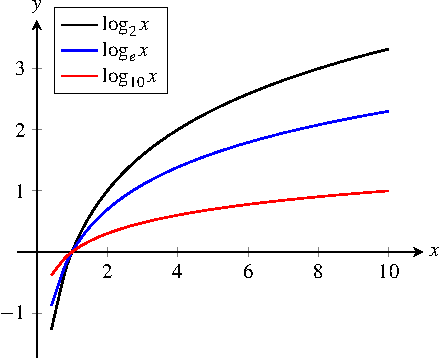
\includegraphics[scale=1.1]{image/12/logarithm.pdf}
\caption{%%
  Graphs of the binary logarithmic function $f(x) = \log_2 x$, the
  natural logarithmic function $f(x) = \log_e x$, and the common
  logarithmic function $f(x) = \log_{10} x$.
}
\label{fig:logarithm:graphs}
\end{figure}

\begin{example}
\textbf{Measuring acidity with pH.}
The pH of a liquid~(or aqueous solution) is a numerical value that is
used to classify whether the liquid is acidic, neutral, or
basic~(alkaline).\footnote{
  See page~670 of the book:
  R.~Chang and K.~A.~Goldsby. \emph{Chemistry}. $12$-th edition,
  McGraw-Hill Education, 2016.  Despite what some chemistry textbooks
  might tell you, a negative value of pH does exist; see the following
  paper: \url{https://doi.org/10.1021/ed083p1465}.
}
If $\molarH$ represents the molar concentration of hygrogen ions, then
the pH of $\molarH$ is defined as
%%
\begin{equation}
\label{eqn:logarithm:pH}
\text{pH}
=
-\log_{10} \molarH.
\end{equation}
%%
If an aqueous solution has a pH $< 7$, the solution is classified as
acidic.  If the solution has a pH $ = 7$, it is classified as
neutral.  An aqueous solution that has a pH $> 7$ is classified as
basic~(or alkaline).  A glass of lemon juice has a hydrogen ion
concentration of $5.4 \times 10^{-3}$
molar~(or $5.4 \times 10^{-3}$M).  Calculate the pH of the lemon juice
and classify its acidity.
\end{example}

\begin{solution}
You have $\molarH = 5.4 \times 10^{-3}$M.  Substitute the number into
\Equation{eqn:logarithm:pH} and you get
%%
\begin{align*}
\text{pH}
&=
-\log_{10} (5.4 \times 10^{-3}) \\[4pt]
&\approx
2.3
\end{align*}
%%
rounded to one decimal place.  Since the pH of the lemon juice is less
than $7$, the lemon juice is classified as acidic.
\end{solution}

\begin{exercise}
\textbf{The pH of blood.}
A specimen of blood has a hydrogen ion concentration of
$4 \times 10^{-8}$M.  Calculate the pH of the specimen and classify
its acidity.
\end{exercise}

\ifbool{showSolution}{
\begin{solution}
Substitute the expression $\molarH = 4 \times 10^{-8}$M into
\Equation{eqn:logarithm:pH} and you have
%%
\begin{align*}
\text{pH}
&=
-\log_{10} (4 \times 10^{-8}) \\[4pt]
&\approx
7.4
\end{align*}
%%
rounded to one decimal place.  As the pH of the blood specimen is
greater than $7$, the specimen is classified as basic.
\end{solution}
}{}

\begin{theorem}
\label{thm:logarithm:lob_b_b_power_x}
Let $b > 0$ be any real number such that $b \neq 1$ and let $x$ be a
real variable.  Then $\log_b (b^x) = x$.
\end{theorem}

Why is \Theorem{thm:logarithm:lob_b_b_power_x} important?
\Theorem{thm:logarithm:lob_b_b_power_x} is often used to solve
equations that involve exponential functions.  In fact, you have
already seen how the theorem was used to solve
\Equation{eqn:exponential_growth_100_10_x} for $x$.  Here are some
more examples.

\begin{example}
Solve the equation $2^x = 64$ for $x$.
\end{example}

\begin{solution}
The equation $2^x = 64$ asks for a value of $x$ such that when $2$ is
raised to the power of $x$, the result will be $64$.  Since the base
is $2$, take the logarithm to base $2$ of both sides of the equation
and you get $\log_2(2^x) = \log_2 64$.  Use
\Theorem{thm:logarithm:lob_b_b_power_x} to simplify the left-hand side
as $\log_2(2^x) = x$, hence you can write $x = \log_2 64$.  You can
use a calculator or computer program to determine that
$x = \log_2 64 = 6$.  As a check, you can see that $2^6 = 64$.
\end{solution}

\begin{example}
\textbf{Population of Australia.}
According to the Australian Bureau of Statistics~(ABS), at the end of
September 2017 the population of Australia grew by $1.6\%$ since the
previous year.\footnote{
  ``3101.0 - Australian Demographic Statistics, Sep 2017'',
  \url{http://web.archive.org/web/20180420062713/http://www.abs.gov.au/AUSSTATS/abs@.nsf/Lookup/3101.0Main+Features1Sep\%202017},
  accessed 2018-04-20.
}
The population by the end of the given period was estimated to be
$24.7029$ million people.  Assume that for the next few years the
population of Australia will grow by a constant rate of $1.6\%$ per
annum.  When will the population of Australia be $30$ million people?
\end{example}

\begin{solution}
You have seen this example before and know that the population~(in
millions) in $t$ years from $2017$ onwards can be written as
\[
P(t)
=
24.7029 \times 1.016^t.
\]
Note that the base is $b = 1.016$.  You want to determine the number
of years $t$ such that $P(t) = 30$ million people.  In other words,
you want to solve the equation
\[
30
=
24.7029 \times 1.016^t
\]
for $t$.  Divide both sides by $24.7029$ to get
$\frac{30}{24.7029} = 1.016^t$.  Now take the logarithm to base
$b = 1.016$ of both sides and you end up with
\[
\log_{1.016} \frac{30}{24.7029}
=
\log_{1.016} (1.016^t).
\]
Use \Theorem{thm:logarithm:lob_b_b_power_x} to simplify the right-hand
side to $\log_{1.016} (1.016^t) = t$ and you can now write
%%
\begin{equation}
\label{eqn:logarithm:Australia_population_doubling_time}
\log_{1.016} \frac{30}{24.7029}
=
t.
\end{equation}
%%
The latter expression evaluates to approximately $t \approx 12.2392$,
rounded to four decimal places.  As a check, you can see that in
approximately $t = 12.2392$ years the population of Australia will be
\[
24.7029 \times 1.016^{12.2392}
\approx
30.000011
\]
million people, rounded to six decimal places.  Therefore some time in
the year $2017 + 12 = 2029$ the population of Australia will be
approximately $30$ million people.
\end{solution}

\begin{exercise}
\textbf{Bacterial growth.}
A Petri dish initially contains ten cells of a type of bacteria.  The
bacteria population is known to have a constant percentage growth rate
of $56\%$ per hour.
%%
\begin{packedenum}
\item\label{subex:logarithm:bacterial_growth_at_least_100_cells}
  Use logarithm to calculate the amount of time required for the
  bacteria population to be at least $100$ cells.

\item\label{subex:logarithm:bacterial_growth_doubling_time}
  Use logarithm to calculate the doubling time of the bacteria
  population.
\end{packedenum}
\end{exercise}

\ifbool{showSolution}{
\begin{solution}
\solutionpart{subex:logarithm:bacterial_growth_at_least_100_cells}
From a previous example, you know that the bacteria population can be
written as $Q(t) = 10 \times 1.56^t$.  Now you want to solve the
equation
\[
100
=
10 \times 1.56^t
\]
for $t$.  Divide both sides of the latter equation by $10$ to get
$\frac{100}{10} = 1.56^t$, which simplifies to $10 = 1.56^t$.  In the
exponential function $1.56^t$, the base is $b = 1.56$.  Take the
logarithm to base $b = 1.56$ of both sides of $10 = 1.56^t$ and you
end up with $\log_{1.56} 10 = \log_{1.56} (1.56^t)$, which by
\Theorem{thm:logarithm:lob_b_b_power_x} can be simplified as
$\log_{1.56} 10 = t$.  Thus $t$ is approximately $t \approx 5.1780$,
rounded to four decimal places.  As a check, note that
$Q(5.1780) = 10 \times 1.56^{5.1780} \approx 99.9998$, rounded to four
decimal places.  However, if $t = 5.1781$ then you have
$Q(5.1781) = 10 \times 1.56^{5.1781} \approx 100.0043$, rounded to
four decimal places.  In other words, you must wait a minimum of
$5.1781$ hours in order for the bacteria population to be at least
$100$ cells.

\solutionpart{subex:logarithm:bacterial_growth_doubling_time}
The initial bacteria population is $a = 10$ cells.  Double this and
you get $2a = 2 \times 10 = 20$ cells.  You want to know the amount of
time required in order for the bacteria population to double from $10$
cells to $20$ cells.  That is, you want to solve the equation
\[
20
=
10 \times 1.56^t
\]
for $t$.  Divide both sides of the latter equation by $10$ to get
$\frac{20}{10} = 1.56^t$, which simplifies to $2 = 1.56^t$.  Taking
the logarithm to base $b = 1.56$ of both sides yields
$\log_{1.56} 2 = \log_{1.56} (1.56^t)$ and use
\Theorem{thm:logarithm:lob_b_b_power_x} to simplify the last equation
to $\log_{1.56} 2 = t$.  Then $t$ is approximately
$t \approx 1.5587$, rounded to four decimal places.  As a check, you
have $Q(1.5587) = 10 \times 1.56^{1.5587} \approx 19.9997$, rounded to
four decimal places.  However, if $t = 1.5588$ then you get
$Q(1.5588) = 10 \times 1.56^{1.5588} \approx 20.0006$, rounded to four
decimal places.  Conclude that the doubling time of the bacteria
population is approximately $1.5588$ hours.
\end{solution}
}{}

\begin{example}
\textbf{Radiocarbon dating.}
Carbon-$14$ decays at a rate of approximately $r = 0.00012097$ per
annum, rounded to eight decimal places.  Calculate the half-life of
$300$ isotopes of carbon-$14$.
\end{example}

\begin{solution}
Radioactive decay follows an exponential decay model of the form
\[
A(t)
=
a e^{-rt}.
\]
Here, $a$ represents the initial number of radioactive isotopes,
$r > 0$ denotes the decay rate as a decimal, and $A(t)$ represents the
remaining number of radioactive isotopes after $t$ units of time.  In
the example, you initially have $a = 300$ isotopes of carbon-$14$ and
the decay rate is $r = 0.00012097$ per annum.  After $t$ years, the
number of remaining carbon-$14$ isotopes can be written as
\[
A(t)
=
300 e^{-0.00012097 t}.
\]
You want to know the number of years required for the initial $300$
isotopes to decay to $\frac{300}{2} = 150$ isotopes.  That is, you
want to solve the equation
\[
150
=
300 e^{-0.00012097 t}
\]
for $t$.  Divide both sides by $300$ to get
$\frac{150}{300} = e^{-0.00012097 t}$, which simplifies to
$\frac{1}{2} = e^{-0.00012097 t}$.  In the exponential function
$e^{-0.00012097 t}$, the base is the irrational number $e$.  Take the
logarithm to base $e$ of both sides of
$\frac{1}{2} = e^{-0.00012097 t}$ and you end up with
$\ln \bigparen{\frac{1}{2}} = \ln \bigparen{e^{-0.00012097 t}}$,
which by \Theorem{thm:logarithm:lob_b_b_power_x} simplifies to
$\ln \bigparen{\frac{1}{2}} = -0.00012097 t$.  Solving the latter
equation for $t$ yields
\[
-\frac{1}{0.00012097}
\ln \parenthesis*{\frac{1}{2}}
=
t
\]
which evaluates to approximately $t \approx 5730$ years, rounded to
the nearest integer.  Conclude that the initial $300$ carbon-$14$
isotopes have a half-life of approximately $5730$ years.
\end{solution}

\begin{exercise}
\textbf{Fermium-$250$.}
Fermium-$250$ is known to have a decay rate of approximately $0.0231$
per minute.  Calculate the half-life of $100$ isotopes of
fermium-$250$.
\end{exercise}

\ifbool{showSolution}{
\begin{solution}
If $A(t)$ represents the number of remaining fermium-$250$ isotopes
after $t$ minutes, then $A(t)$ can be written as
\[
A(t)
=
100 e^{-0.0231 t}.
\]
Half of $100$ is $100 / 2 = 50$ and you want to solve the equation
\[
50
=
100 e^{-0.0231 t}
\]
for $t$.  In the latter equation, divide both sides by $100$ to get
$\frac{50}{100} = e^{-0.0231 t}$, which simplifies to
$\frac{1}{2} = e^{-0.0231 t}$.  Take the logarithm to base $e$ of both
sides and you end up with
$\ln \parenthesis*{\frac{1}{2}} = \ln \parenthesis*{e^{-0.0231 t}}$,
which by \Theorem{thm:logarithm:lob_b_b_power_x} simplifies to
$\ln \parenthesis*{\frac{1}{2}} = -0.0231 t$.  The last equation
can be solved for $t$ to get
\[
t
=
-\frac{1}{0.0231}
\ln \parenthesis*{\frac{1}{2}}
\]
which evaluates to approximately $t \approx 30$, rounded to the
nearest integer.  Therefore the half-life of $100$ isotopes of
fermium-$250$ is approximately $30$ minutes.
\end{solution}
}{}


%%%%%%%%%%%%%%%%%%%%%%%%%%%%%%%%%%%%%%%%%%%%%%%%%%%%%%%%%%%%%%%%%%%%%%%%%%%

\section{Properties of logarithm}

One of the most useful properties of logarithm is that exponentiation
and logarithm are inverse functions of each other.  This is similar to
the way addition and subtraction are inverse operations of each other,
or multiplication and division are inverse operations of each other.
Consequently, you can use this inverse property between exponentiation
and logarithm to solve equations that involve exponential and
logarithmic functions.  What does all this mean?

Consider the example of addition and subtraction.  Suppose you have
two numbers $a$ and $x$ such that $a \neq 0$.  Adding $a$ to $x$
results in $x + a$.  You can undo the addition by subtracting $a$ from
$x + a$.  Doing so gives you the expression
\[
(x + a) - a
=
x + a - a
=
x.
\]
On the other hand, suppose you subtract $a$ from $x$ and end up with
$x - a$.  Undoing the subtraction requires that you add $a$ to
$x - a$.  Doing so results in
\[
(x - a) + a
=
x - a + a
=
x.
\]
The core idea is that addition and subtraction are inverse operations
of each other.  This inverse property between addition and subtraction
allows you to undo the result of any of the two operations.

As another example, consider multiplication and division.  Let $a$ and
$x$ be any numbers such that $a \neq 0$ and $x \neq 0$.  Multiplying
$x$ by $a$ results in $ax$.  To undo the multiplication, you divide
$ax$ by $a$ to produce
\[
\frac{ax}{a}
=
\frac{a}{a} \times x
=
x.
\]
On the other hand, suppose that you divide $x$ by $a$ to get $x / a$.
To undo the division, you multiply $x / a$ by $a$ to get
\[
\frac{x}{a} \times a
=
\frac{a}{a} \times x
=
x.
\]
Thus you see that multiplication and division are inverse operations
of each other.  This inverse property between multiplication and
division allows you to undo the result of any of the two operations.

The fact that exponentiation and logarithm are inverses of each other
is summarised in \Theorem{thm:logarithm:lob_b_b_power_x}.  This
inverse property between exponentiation and logarithm can be
visualised as the graph shown in
\Figure{fig:logarithmic_function_reflection_of_exponential_function}
for the specific case of the natural logarithmic function
$f(x) = \ln x$ and the exponential function $g(x) = e^x$.  The graphs
for exponentiation and logarithm to other bases are similar.
\Figure{fig:logarithmic_function_reflection_of_exponential_function}
shows that you can obtain the graph of $g(x)$ by reflecting the graph
of $f(x)$ about the diagonal line $y = x$.  Furthermore, you can also
produce the graph of $f(x)$ by reflecting the graph of $g(x)$ about
the line $y = x$.  This means that, for example, given the point
$\tuple{0}{1}$ on the graph of $g(x)$, the corresponding point on the
graph of $f(x)$ is obtained by interchanging the $x$- and
$y$-coordinates to get $\tuple{1}{0}$.  In fact,
\Theorem{thm:logarithm:lob_b_b_power_x} is part of another theorem
that can be used to cancel exponentiation and logarithm whenever these
two operations occur together.  This other result is
\Theorem{thm:logarithm:cancellation_property} below.

\begin{figure}[!htbp]
\centering
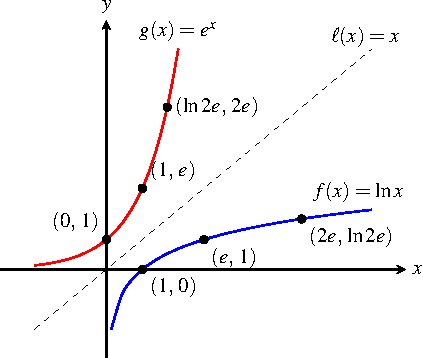
\includegraphics[scale=1.2]{image/12/inverses.pdf}
\caption{%%
  The graph of the natural logarithmic function $f(x) = \ln x$ is
  obtained by reflecting the exponential function $g(x) = e^x$ with
  respect to the line $\ell(x) = x$.
}
\label{fig:logarithmic_function_reflection_of_exponential_function}
\end{figure}

\begin{exercise}
Provide an example of two operations~(different from those presented
above) that are inverses of each other.  Explain how one operation can
be used to undo the result of the other operation.
\end{exercise}

\ifbool{showSolution}{
\begin{solution}
The operations of squaring and square root are inverses of each
other.  Let $x \geq 0$ be any real number.  The square of $x$ is
$x^2$.  To undo the squaring, take the square root of $x^2$ and you
get
\[
\sqrt{x^2}
=
(x^2)^{1/2}
=
x^{2/2}
=
x.
\]
On the other hand, the square root of $x$ is $\sqrt{x}$.  To undo the
square root, you square $\sqrt{x}$ and end up with
\[
\bigparen{\sqrt{x}}^2
=
\bigparen{x^{1/2}}^2
=
x^{2/2}
=
x.
\]
Thus either operation can be used to undo the result of the other
operation.
\end{solution}
}{}

\begin{theorem}
\label{thm:logarithm:cancellation_property}
\textbf{Cancellation property.}
Let $b$ be a positive number such that $b \neq 1$.
%%
\begin{packedenum}
\item\label{subthm:logarithm:cancellation_property_log_exponential}
  If $x$ is any real number, then $\log_b (b^x) = x$.

\item\label{subthm:logarithm:cancellation_property_exponential_log}
  If $x > 0$ is any positive number, then $b^{\log_b x} = x$.
\end{packedenum}
\end{theorem}

\begin{example}
Solve the equation $\log_{10} x = \frac{1}{2}$ for $x$.
\end{example}

\begin{solution}
The equation $\log_{10} x = \frac{1}{2}$ asks you to determine a value
of $x$ such that $\log_{10} x$ evaluates to $1 / 2$.  You can use
\Subtheorem{thm:logarithm:cancellation_property}{subthm:logarithm:cancellation_property_exponential_log}
and consider both sides of $\log_{10} x = \frac{1}{2}$ as exponents of
the base $10$.  Then the latter equation can be written as
\[
10^{\log_{10} x}
=
10^{1/2}
=
\sqrt{10}.
\]
The left-hand side simplifies to $x$ and the equation now becomes
$x = \sqrt{10}$.
\end{solution}

\begin{exercise}
Solve the equation $\log_2 x = 5$ for $x$.
\end{exercise}

\ifbool{showSolution}{
\begin{solution}
You can treat both sides of $\log_2 x = 5$ as exponents of the base
$2$.  Then the latter equation can also be written as
\[
2^{\log_2 x}
=
2^5
\]
which by
\Subtheorem{thm:logarithm:cancellation_property}{subthm:logarithm:cancellation_property_exponential_log}
simplifies to $x = 2^5 = 32$.
\end{solution}
}{}

\begin{exercise}
Solve the equation $\ln 2x = 3$ for $x$.
\end{exercise}

\ifbool{showSolution}{
\begin{solution}
You can treat both sides of the equation $\ln 2x = 3$ as exponents of
the irrational number $e$.  This allows you to write the latter
equation as
\[
e^{\ln 2x}
=
e^3.
\]
Use
\Subtheorem{thm:logarithm:cancellation_property}{subthm:logarithm:cancellation_property_exponential_log}
to simplify the last equation to $2x = e^3$, which upon solving for
$x$ yields $x = \frac{1}{2} e^3$.
\end{solution}
}{}

\begin{exercise}
\textbf{Negative pH.}
In the Richmond Mine at Iron Mountain, California, USA a team of
researchers found that the underground water had a pH value as low as
$-3.6$.\footnote{
  See the paper: \url{https://doi.org/10.1021/es990646v}.
}
Suppose that the water had a pH value of $-3.6$.  Calculate the molar
concentration of hydrogren ions in the water.
\end{exercise}

\ifbool{showSolution}{
\begin{solution}
You have $\text{pH} = -3.6$.  Substitute the latter value into
\Equation{eqn:logarithm:pH} to obtain the equation
\[
-3.6
=
-\log_{10} x
\]
where $x = \molarH$.  The above equation simplifies to
$3.6 = \log_{10} x$, where you can consider both sides as exponents of
$10$.  In other words, you have the equivalent equation
$10^{3.6} = 10^{\log_{10} x}$, which by
\Subtheorem{thm:logarithm:cancellation_property}{subthm:logarithm:cancellation_property_exponential_log}
can be simplified as $10^{3.6} = x$.  Conclude that if the underground
water at Iron Mountain had a pH value of $-3.6$, then the water had a
hydrogen ion concentration of $10^{3.6}$M.
\end{solution}
}{}

\begin{theorem}
\label{thm:logarithm:properties}
\textbf{Properties of logarithm.}
Let $\triple{a}{b}{c}$ be positive numbers such that $b \neq 1$.
%%
\begin{packedenum}
\item\label{thm:logarithm:properties_addition}
  Addition rule:
  $\log_b (ac) = \log_b a + \log_b c$

\item\label{thm:logarithm:properties_subtraction}
  Subtraction rule:
  $\log_b \parenthesis*{\frac{a}{c}} = \log_b a - \log_b c$

\item\label{thm:logarithm:properties_multiplication}
  Power rule:
  If $x$ is any real number, then $\log_b (a^x) = x \cdot \log_b a$.

\item\label{thm:logarithm:properties_log_1}
  Zero rule: $\log_b 1 = 0$

\item\label{thm:logarithm:properties_log_b}
  Unit rule: $\log_b b = 1$
\end{packedenum}
\end{theorem}

\begin{proof}
\solutionpart{thm:logarithm:properties_addition}
Since $\triple{a}{b}{c}$ are positive numbers, there exist numbers $m$
and $n$ such that $a = b^m$ and $c = b^n$.  By
\Subtheorem{thm:logarithm:cancellation_property}{subthm:logarithm:cancellation_property_log_exponential}
you have the identities
%%
\begin{equation}
\label{eqn:logarithm:log_b_a_m_log_b_c_n}
\log_b a = \log_b (b^m) = m
%%
\qquad
\text{and}
\qquad
%%
\log_b c = \log_b (b^n) = n.
\end{equation}
%%
The product of $a$ and $c$ can be written as
$a \cdot c = b^m \cdot b^n$, which simplifies to
$a \cdot c = b^{m + n}$.  In the latter equation, taking the logarithm
to base $b$ of both sides results in
$\log_b (a \cdot c) = \log_b (b^{m+n})$.  Use
\Subtheorem{thm:logarithm:cancellation_property}{subthm:logarithm:cancellation_property_log_exponential}
again to simplify the last equation to $\log_b (a \cdot c) = m+n$,
which by the identities in~\eqref{eqn:logarithm:log_b_a_m_log_b_c_n}
can be written as
$\log_b (a \cdot c) = \log_b a + \log_b c$.

\solutionpart{thm:logarithm:properties_subtraction}
See \Exercise{ex:logarithm:properties_subtraction}.

\solutionpart{thm:logarithm:properties_multiplication}
Since $a$ and $b$ are positive numbers, there exists a number $n$ such
that $a = b^n$.  If $x$ is any real number, raise both sides of the
latter equation to the power of $x$ and you get
$a^x = (b^n)^x$, which simplifies to $a^x = b^{nx}$.  In the last
equation, take the logarithm to base $b$ of both sides and you obtain
$\log_b (a^x) = \log_b (b^{nx})$, which by
\Subtheorem{thm:logarithm:cancellation_property}{subthm:logarithm:cancellation_property_log_exponential}
can also be written as
%%
\begin{equation}
\label{eqn:logarithm:log_b_a_x_nx}
\log_b (a^x)
=
nx.
\end{equation}
%%
In the equation $a = b^n$, taking the logarithm to base $b$ of both
sides produces $\log_b a = \log_b (b^n)$ and using
\Subtheorem{thm:logarithm:cancellation_property}{subthm:logarithm:cancellation_property_log_exponential}
again shows that you can also write $\log_b a = n$.  Substitute the
latter expression into \Equation{eqn:logarithm:log_b_a_x_nx} and you
get $\log_b (a^x) = (\log_b a) \cdot x$, which you can also write as
$\log_b (a^x) = x \cdot \log_b a$.

\solutionpart{thm:logarithm:properties_log_1}
See \Exercise{ex:logarithm:log_b_1_0}.

\solutionpart{thm:logarithm:properties_log_b}
As $b \neq 1$ is positive, use
\Subtheorem{thm:logarithm:cancellation_property}{subthm:logarithm:cancellation_property_exponential_log}
to write $b^{\log_b b} = b$.  Taking the logarithm to base $b$ of both
sides yields $\log_b (b^{\log_b b}) = \log_b b$, which by the power
rule from \Part{thm:logarithm:properties_multiplication} can also be
written as $\log_b b \cdot \log_b b = \log_b b$.  Since $b \neq 1$,
by \Part{thm:logarithm:properties_log_1} you know that
$\log_b b \neq 0$.  Thus in the equation
$\log_b b \cdot \log_b b = \log_b b$ you can divide both sides by
$\log_b b$ to get
\[
\frac{
  \log_b b \cdot \log_b b
}{
  \log_b b
}
=
\frac{\log_b b}{\log_b b}
\]
and simplify the latter expression to $\log_b b = 1$.
\end{proof}

\begin{exercise}
\label{ex:logarithm:properties_subtraction}
Prove
\Subtheorem{thm:logarithm:properties}{thm:logarithm:properties_subtraction}.
\end{exercise}

\ifbool{showSolution}{
\begin{solution}
Since $\triple{a}{b}{c}$ are positive numbers, there exist numbers $m$
and $n$ such that $a = b^m$ and $c = b^n$.  Now use
\Subtheorem{thm:logarithm:cancellation_property}{subthm:logarithm:cancellation_property_log_exponential}
to obtain the identities
%%
\begin{equation}
\label{eqn:logarithm:ex_log_b_a_m_log_b_c_n}
\log_b a = \log_b (b^m) = m
%%
\qquad
\text{and}
\qquad
%%
\log_b c = \log_b (b^n) = n.
\end{equation}
%%
You can write the fraction $a / c$ as
$\frac{a}{c} = \frac{b^m}{b^n}$, which simplifies to
$\frac{a}{c} = b^{m - n}$.  In the latter equation, take the logarithm
to base $b$ of both sides and you end up with
$\log_b \parenthesis*{\frac{a}{c}} = \log_b (b^{m - n})$.  Another
application of
\Subtheorem{thm:logarithm:cancellation_property}{subthm:logarithm:cancellation_property_log_exponential}
shows that the latter equation can be simplified as
$\log_b \parenthesis*{\frac{a}{c}} = m - n$, which by the identities
in~\eqref{eqn:logarithm:ex_log_b_a_m_log_b_c_n} can also be written as
$\log_b \parenthesis*{\frac{a}{c}} = \log_b a - \log_b c$.
\end{solution}
}{}

\begin{exercise}
\label{ex:logarithm:log_b_1_0}
Prove
\Subtheorem{thm:logarithm:properties}{thm:logarithm:properties_log_1}.
\end{exercise}

\ifbool{showSolution}{
\begin{solution}
Let $b > 0$ be any number such that $b \neq 1$.  You know that
$b^0 = 1$.  Take the logarithm to base $b$ of both sides and you
obtain $\log_b (b^0) = \log_b 1$, which by the power rule from
\Subtheorem{thm:logarithm:properties}{thm:logarithm:properties_multiplication}
can also be written as $0 \cdot \log_b b = \log_b 1$.  The latter
equation simplifies to $0 = \log_b 1$.
\end{solution}
}{}

\begin{theorem}
\label{thm:logarithm:change_of_base}
\textbf{Change of base.}
Let $b \neq 1$ and $k \neq 1$ be positive numbers.  If $x > 0$ is any
number, then
\[
\log_b x
=
\frac{
  \log_k x
}{
  \log_k b
}.
\]
\end{theorem}

\begin{proof}
Use
\Subtheorem{thm:logarithm:cancellation_property}{subthm:logarithm:cancellation_property_exponential_log}
to write $b^{\log_b x} = x$.  Take the logarithm to base $k$ of both
sides and you end up with
$\log_k \parenthesis*{b^{\log_b x}} = \log_k x$, which
by
\Subtheorem{thm:logarithm:properties}{thm:logarithm:properties_multiplication}
can also be written as
\[
\log_b x \cdot \log_k b
=
\log_k x.
\]
Solve the latter equation for $\log_b x$ to get the result.
\end{proof}

\Theorem{thm:logarithm:change_of_base} is most useful in cases where
an electronic calculator or computer program cannot directly evaluate
the logarithm of a number to any positive base you want.  The reason
might be that the calculator~(respectively, program) does not have a
buttom or command to evaluate the logarithm to an arbitrary base.
Consider again
\Equation{eqn:logarithm:Australia_population_doubling_time}, which is
repeated below for reference:
\[
\log_{1.016} \frac{30}{24.7029}
=
t.
\]
Here, the base of the logarithm is $b = 1.016$.  Use
\Subtheorem{thm:logarithm:properties}{thm:logarithm:properties_subtraction}
to write the latter equation as
%%
\begin{equation}
\label{eqn:logarithm:Australia_population_doubling_time_change_of_base}
\begin{aligned}
\log_{1.016} \frac{30}{24.7029}
&=
\log_{1.016} 30 - \log_{1.016} 24.7029 \\[4pt]
&=
t.
\end{aligned}
\end{equation}
%%
If your calculator or computer program does not have a buttom or
command for the logarithm to base $1.016$, use
\Theorem{thm:logarithm:change_of_base} to change the base to a more
convenient base such as base $e$.  With the base of $e$, you can now
write
\[
\log_{1.016} 30
=
\frac{
  \ln 30
}{
  \ln 1.016
}
%%
\qquad
\text{and}
\qquad
%%
\log_{1.016} 24.7029
=
\frac{
  \ln 24.7029
}{
  \ln 1.016
}
\]
which can be used to write
\Expression{eqn:logarithm:Australia_population_doubling_time_change_of_base}
as
%%
\begin{align*}
t
&=
\frac{
  \ln 30
}{
  \ln 1.016
}
-
\frac{
  \ln 24.7029
}{
  \ln 1.016
} \\[4pt]
&=
\frac{
  \ln 30 - \ln 24.7029
}{
  \ln 1.016
}.
\end{align*}
%%
The latter expression can be evaluated by any calculator or computer
program that implements the natural logarithm.

\begin{exercise}
Consider the expression $\log_2 256$.  Without using a calculator or
computer program:
%%
\begin{packedenum}
\item\label{subex:logarithm:log_2_256_properties}
  Simplify the expression by means of the properties of logarithm.

\item\label{subex:logarithm:log_2_256_change_base}
  Simplify the expression by first changing the base from $2$ to $e$.
\end{packedenum}
\end{exercise}

\ifbool{showSolution}{
\begin{solution}
\solutionpart{subex:logarithm:log_2_256_properties}
Note that $256 = 2^8$.  You can write $\log_2 256 = \log_2 (2^8)$.
Use the power rule of
\Subtheorem{thm:logarithm:properties}{thm:logarithm:properties_multiplication}
to write $\log_2 (2^8) = 8 \cdot \log_2 2$, which by the unit rule of
\Subtheorem{thm:logarithm:properties}{thm:logarithm:properties_log_b}
simplifies to $\log_2 (2^8) = 8 \cdot 1 = 8$.  Therefore $\log_2 256$
evaluates to $\log_2 256 = 8$.

\solutionpart{subex:logarithm:log_2_256_change_base}
By using \Theorem{thm:logarithm:change_of_base}, you change the base
of $\log_2 256$ to base $e$ as follows:
\[
\log_2 256
=
\frac{
  \ln 256
}{
  \ln 2
}.
\]
Since $\ln 256 = \ln (2^8)$, use the power rule of
\Subtheorem{thm:logarithm:properties}{thm:logarithm:properties_multiplication}
to write
\[
\log_2 256
=
\frac{
  \ln (2^8)
}{
  \ln 2
}
=
\frac{
  8 \cdot \ln 2
}{
  \ln 2
}.
\]
The right-hand side simplifies to $8$, hence $\log_2 256 = 8$.
\end{solution}
}{}

\begin{exercise}
\textbf{Newton's law of cooling.}
Let $T_0$ be the original temperature of an object and suppose that
$T_s$ represent the constant temperature of the environment
surrounding the object, all temperatures measured in degrees Celsius.
If $T(t)$ represents the temperature of an object after $t$ units of
time, Newton's law of cooling states that $T(t)$ can be written as
%%
\begin{equation}
\label{eqn:logarithm:Newton_law_cooling}
T(t)
=
T_s + (T_0 - T_s) e^{-kt}
\end{equation}
%%
where $k > 0$ is the rate of cooling written as a decimal.  Here, it
is assumed that the surrounding maintains a constant temperature.
Suppose a pot of soup has a tempature of $\degreec{100}$ and that the
temperature of the surrounding is $\degreec{15}$.  You place the pot
of soup on the kitchen bench and let the soup cool.  After one hour, the
temperature of the soup drops down to $\degreec{50}$.
%%
\begin{packedenum}
\item\label{subex:logarithm:Newton_law_cooling_soup_formula}
  Assume that the surrounding maintains a constant temperature of
  $\degreec{15}$.  Derive a formula for the temperature $T(t)$ of the
  soup after $t$ hours.

\item\label{subex:logarithm:Newton_law_cooling_soup_20}
  If the surrounding continues to maintain a constant temperature of
  $\degreec{15}$, how long must you wait for the temperature of the
  soup to be $\degreec{20}$?
\end{packedenum}
\end{exercise}

\ifbool{showSolution}{
\begin{solution}
\solutionpart{subex:logarithm:Newton_law_cooling_soup_formula}
First, you must determine the rate $k$ of cooling.  The original
temperature of the pot of soup is $T_0 = 100$ degrees Celsius.  The
surrounding maintains a constant temperature of $T_s = 15$ degrees
Celsius.  After one hour, the temperature of the soup decreases to
$\degreec{50}$, which you can write as the expression $T(1) = 50$.
Substitute the known values into
\Equation{eqn:logarithm:Newton_law_cooling} and you end up with
%%
\begin{align*}
50
&=
15 + (100 - 15) e^{-k \times 1} \\[4pt]
&=
15 + 85 e^{-k}.
\end{align*}
%%
You need to solve the latter equation for $k$.  The last equation can
also be written as $50 - 15 = 85 e^{-k}$.  Divide both sides by $85$
and you get $\frac{50 - 15}{85} = e^{-k}$, which simplifies to
$\frac{7}{17} = e^{-k}$.  In the last equation, take the natural
logarithm of both sides and you have
$\ln \parenthesis*{\frac{7}{17}} = \ln (e^{-k})$, which by
\Subtheorem{thm:logarithm:cancellation_property}{subthm:logarithm:cancellation_property_log_exponential}
can be simplified as $\ln \parenthesis*{\frac{7}{17}} = -k$.  Solve
the last equation for $k$ and you get
%%
\begin{equation}
\label{eqn:logarithm:Newton_law_cooling_rate_k}
\begin{aligned}
k
&=
-\ln \parenthesis*{\frac{7}{17}} \\[4pt]
&=
-(\ln 7 - \ln 17) \\[4pt]
&=
\ln 17 - \ln 7 \\[4pt]
&=
\ln \parenthesis*{\frac{17}{7}}.
\end{aligned}
\end{equation}
%%
You now have all information necessary to substitute into
\Equation{eqn:logarithm:Newton_law_cooling}.  Substitution and
simplifying yield the formula
\[
T(t)
=
15 + 85 e^{-kt}
\]
where $k$ is defined as per
\Expression{eqn:logarithm:Newton_law_cooling_rate_k}.

\solutionpart{subex:logarithm:Newton_law_cooling_soup_20}
You want a value of $t$ such that $T(t) = 20$ degrees Celsius.  That
is, you want to solve the equation $20 = 15 + 85 e^{-kt}$ for $t$,
where $k$ is defined as in
\Expression{eqn:logarithm:Newton_law_cooling_rate_k}.  The latter
equation can be written as $20 - 15 = 85 e^{-kt}$ or
$\frac{20 - 15}{85} = e^{-kt}$, which simplifies to
$\frac{1}{17} = e^{-kt}$.  Take the natural logarithm of both sides
and you have $\ln \parenthesis*{\frac{1}{17}} = \ln (e^{-kt})$, which
by
\Subtheorem{thm:logarithm:cancellation_property}{subthm:logarithm:cancellation_property_log_exponential}
simplifies to $\ln \parenthesis*{\frac{1}{17}} = -kt$.  Solving the
last equation for $t$ produces the expression
%%
\begin{align*}
t
&=
-\frac{1}{k} \ln \parenthesis*{\frac{1}{17}} \\[4pt]
&\approx
3.1931
\end{align*}
%%
rounded to four decimal places.  Therefore you must wait approximately
$3.1931$ hours for the soup to cool down to $\degreec{20}$.
\end{solution}
}{}


%%%%%%%%%%%%%%%%%%%%%%%%%%%%%%%%%%%%%%%%%%%%%%%%%%%%%%%%%%%%%%%%%%%%%%%%%%%

\section{Logarithmic plots}

Another useful property of logarithm is that it can scale down large
numbers and scale up small numbers.  This is especially useful if your
data set consists of, for example, numbers that range from the
hundreds to the billions.  In that case, you should consider plotting
your data set with a logarithmic axis.


%%%%%%%%%%%%%%%%%%%%%%%%%%%%%%%%%%%%%%%%%%%%%%%%%%%%%%%%%%%%%%%%%%%%%%%%%%%

\subsection{Logarithmic scaling on vertical axis}

By way of an example, consider the graphs in
\Figure{fig:logarithm:rainbow_trout}.  Each graph shows the same data
set on the total length versus weight of $42$ rainbow trout; see
\Table{tab:logarithm:rainbow_trout}.\footnote{
  The data set was published in the following document:
  \url{http://web.archive.org/web/20180513070421/https://fortress.wa.gov/ecy/publications/documents/0003017.pdf},
  accessed 2018-05-13.
}
\Figure{fig:logarithm:rainbow_trout_linear} shows the scatter plot
with the usual linear scale for the horizontal and vertical axes.  Up
to now, you have been producing scatter plots with linear scaling.
Note that \Figure{fig:logarithm:rainbow_trout_log} shows the same
scatter plot, but each value on the vertical axis has been transformed
to its equivalent under the common logarithm.  The graph in
\Figure{fig:logarithm:rainbow_trout_log} is called a \emph{semi-log}
plot because the common logarithm was taken of each value on only one
axis, in particular the vertical axis.

\begin{figure}[!htbp]
\centering
\subfigure[]{
  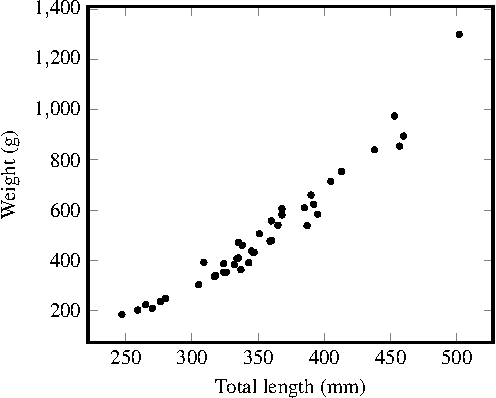
\includegraphics[scale=0.79]{image/12/rainbow-trout-linear.pdf}
  \label{fig:logarithm:rainbow_trout_linear}
}
%%
%%
\subfigure[]{
  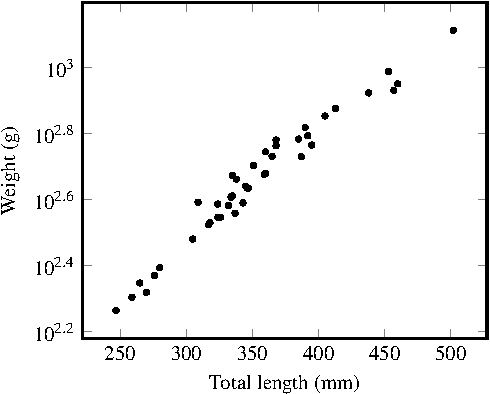
\includegraphics[scale=0.79]{image/12/rainbow-trout-log.pdf}
  \label{fig:logarithm:rainbow_trout_log}
}
\caption{%%
  The total length versus weight of $42$ rainbow trout.  The trout
  were sampled from four different locations along the Spokane River,
  Washington, USA during the months of July, August, and October of
  1999.  The total length of each trout was measured in millimetres
  and the weight was measured in grams.  (a)~A scatter plot with
  linear axes.  (b)~A scatter plot with semi-log axes.
}
\label{fig:logarithm:rainbow_trout}
\end{figure}

As you can see from \Figure{fig:logarithm:rainbow_trout_log}, a
semi-log plot can be used to linearise a data set.  If a data set
approximately follows an exponential model $Q(x)$, a semi-log plot
should allow you to visualise the data set as points around a straight
line.  In other words, if the semi-log plot shows that the points seem
to lie around a straight line, then you should try to model the
original data set via an exponential function.  To do so, first you
must linearise the data by taking the (usually natural) logarithm of
the $y$ column.  Second, you use linear regression to determine a
linear function $f(x)$ that best fits the linearised data.  Finally,
you transform $f(x)$ into the exponential function $Q(x)$.  In
particular, suppose that the data set approximately follows the
exponential function
%%
\begin{equation}
\label{eqn:logarithm:exponential_model}
Q(x)
=
a \cdot e^{rx}.
\end{equation}
%%
The values of the parameters $a$ and $r$ can be estimated as follows.
Take the natural logarithm of both sides of
\Equation{eqn:logarithm:exponential_model} and you get
$\ln Q(x) = \ln (a \cdot e^{rx})$.  Use the addition rule of
\Subtheorem{thm:logarithm:properties}{thm:logarithm:properties_addition}
to write the latter equation as $\ln Q(x) = \ln a + \ln (e^{rx})$,
which by
\Subtheorem{thm:logarithm:cancellation_property}{subthm:logarithm:cancellation_property_log_exponential}
simplifies to
%%
\begin{equation}
\label{eqn:logarithm:exponential_linearised}
\ln Q(x)
=
rx + \ln a.
\end{equation}
%%
Note that~\eqref{eqn:logarithm:exponential_linearised} is a linear
equation, where the vertical intercept and rate of change are $\ln a$
and $r$, respectively.  Use linear regression to estimate $r$ as
$\alphahat$ and $\ln a$ as $\betahat$.  Now $\alphahat$ is an estimate
of $r$ in \Equation{eqn:logarithm:exponential_model} and
$e^{\betahat}$ is an estimate of $a$
in~\eqref{eqn:logarithm:exponential_model}.  The above technique is
called \emph{exponential regression} because you are attempting to fit
an exponential function to a data set.
\Example{ex:logarithm:rainbow_trout} below clarifies the above
technique for estimating the parameters of an exponential model.

\begin{table}[!htbp]
\centering
\begin{tabular}{cccrrrr} \toprule
$x$   & $w$    & $y$      & $d(x_i)$    & $d(y_i)$  & $d(x_i) d(y_i)$ & $d(x_i) d(x_i)$ \\\midrule
$457$ & $855$  & $6.7511$ & $104.1429$  & $0.6301$  & $65.6217$      & $10845.7347$    \\
$405$ & $715$  & $6.5723$ & $52.1429$   & $0.4513$  & $23.5317$      & $2718.8776$     \\
$453$ & $975$  & $6.8824$ & $100.1429$  & $0.7614$  & $76.2536$      & $10028.5918$    \\
$460$ & $895$  & $6.7968$ & $107.1429$  & $0.6758$  & $72.4109$      & $11479.5918$    \\
$335$ & $472$  & $6.1570$ & $-17.8571$  & $0.0360$  & $-0.6427$      & $318.8776$      \\
$365$ & $540$  & $6.2916$ & $12.1429$   & $0.1706$  & $2.0713$       & $147.4490$      \\
$390$ & $660$  & $6.4922$ & $37.1429$   & $0.3713$  & $13.7893$      & $1379.5918$     \\
$368$ & $581$  & $6.3648$ & $15.1429$   & $0.2438$  & $3.6913$       & $229.3061$      \\
$385$ & $609$  & $6.4118$ & $32.1429$   & $0.2908$  & $9.3481$       & $1033.1633$     \\
$360$ & $557$  & $6.3226$ & $7.1429$    & $0.2016$  & $1.4398$       & $51.0204$       \\
$346$ & $433$  & $6.0707$ & $-6.8571$   & $-0.0503$ & $0.3446$       & $47.0204$       \\
$438$ & $840$  & $6.7334$ & $85.1429$   & $0.6124$  & $52.1426$      & $7249.3061$     \\
$392$ & $623$  & $6.4345$ & $39.1429$   & $0.3136$  & $12.2735$      & $1532.1633$     \\
$324$ & $387$  & $5.9584$ & $-28.8571$  & $-0.1626$ & $4.6911$       & $832.7347$      \\
$360$ & $479$  & $6.1717$ & $7.1429$    & $0.0507$  & $0.3622$       & $51.0204$       \\
$413$ & $754$  & $6.6254$ & $60.1429$   & $0.5044$  & $30.3363$      & $3617.1633$     \\
$276$ & $235$  & $5.4596$ & $-76.8571$  & $-0.6614$ & $50.8336$      & $5907.0204$     \\
$387$ & $538$  & $6.2879$ & $34.1429$   & $0.1669$  & $5.6974$       & $1165.7347$     \\
$345$ & $438$  & $6.0822$ & $-7.8571$   & $-0.0388$ & $0.3046$       & $61.7347$       \\
$395$ & $584$  & $6.3699$ & $42.1429$   & $0.2489$  & $10.4899$      & $1776.0204$     \\
$326$ & $353$  & $5.8665$ & $-26.8571$  & $-0.2545$ & $6.8357$       & $721.3061$      \\
$270$ & $209$  & $5.3423$ & $-82.8571$  & $-0.7787$ & $64.5171$      & $6865.3061$     \\
$359$ & $476$  & $6.1654$ & $6.1429$    & $0.0444$  & $0.2729$       & $37.7347$       \\
$347$ & $432$  & $6.0684$ & $-5.8571$   & $-0.0526$ & $0.3079$       & $34.3061$       \\
$259$ & $202$  & $5.3083$ & $-93.8571$  & $-0.8127$ & $76.2797$      & $8809.1633$     \\
$247$ & $184$  & $5.2149$ & $-105.8571$ & $-0.9061$ & $95.9122$      & $11205.7347$    \\
$280$ & $248$  & $5.5134$ & $-72.8571$  & $-0.6076$ & $44.2651$      & $5308.1633$     \\
$265$ & $223$  & $5.4072$ & $-87.8571$  & $-0.7138$ & $62.7139$      & $7718.8776$     \\
$309$ & $392$  & $5.9713$ & $-43.8571$  & $-0.1497$ & $6.5666$       & $1923.4490$     \\
$338$ & $460$  & $6.1312$ & $-14.8571$  & $0.0102$  & $-0.1521$      & $220.7347$      \\
$334$ & $406$  & $6.0064$ & $-18.8571$  & $-0.1146$ & $2.1617$       & $355.5918$      \\
$332$ & $383$  & $5.9480$ & $-20.8571$  & $-0.1730$ & $3.6073$       & $435.0204$      \\
$324$ & $353$  & $5.8665$ & $-28.8571$  & $-0.2545$ & $7.3447$       & $832.7347$      \\
$337$ & $363$  & $5.8944$ & $-15.8571$  & $-0.2266$ & $3.5930$       & $251.4490$      \\
$343$ & $390$  & $5.9661$ & $-9.8571$   & $-0.1548$ & $1.5263$       & $97.1633$       \\
$318$ & $340$  & $5.8289$ & $-34.8571$  & $-0.2920$ & $10.1798$      & $1215.0204$     \\
$305$ & $303$  & $5.7137$ & $-47.8571$  & $-0.4073$ & $19.4901$      & $2290.3061$     \\
$335$ & $410$  & $6.0162$ & $-17.8571$  & $-0.1048$ & $1.8720$       & $318.8776$      \\
$317$ & $335$  & $5.8141$ & $-35.8571$  & $-0.3069$ & $11.0031$      & $1285.7347$     \\
$351$ & $506$  & $6.2265$ & $-1.8571$   & $0.1055$  & $-0.1960$      & $3.4490$        \\
$368$ & $605$  & $6.4052$ & $15.1429$   & $0.2842$  & $4.3042$       & $229.3061$      \\
$502$ & $1300$ & $7.1701$ & $149.1429$  & $1.0491$  & $156.4704$     & $22243.5918$    \\\bottomrule
\end{tabular}

\caption{%%
  The total length $x$ versus weight $w$ of $42$ rainbow trout.  Total
  length is measured in millimetres and weight is measured in grams.
  Each $y_i$ is the natural logarithm of $w_i$.  If $\xbar$ and
  $\ybar$ are the means of the $x$ and $y$ columns, respectively, then
  $d(x_i) = x_i - \xbar$ and $d(y_i) = y_i - \ybar$.  The whole table
  shows the detailed calculation necessary for the linear regression
  of the $x$ and $y$ columns.
}
\label{tab:logarithm:rainbow_trout}
\end{table}

\begin{example}
\label{ex:logarithm:rainbow_trout}
\textbf{Rainbow trout.}
Suppose that the rainbow trout data set shown in
\Figure{fig:logarithm:rainbow_trout} follows the exponential
model~\eqref{eqn:logarithm:exponential_model}.
%%
\begin{packedenum}
\item\label{subex:logarithm:trout_logarithm}
  Take the natural logarithm of each weight value.

\item\label{subex:logarithm:trout_linear_regression}
  Use linear regression to estimate the parameters $a$ and $r$.

\item\label{subex:logarithm:trout_formula_graph}
  Use your estimates
  from \Part{subex:logarithm:trout_linear_regression} to write a
  formula for the weight $Q(x)$~(in grams) of a rainbow trout that has
  a total length of $x$ millimetres.  Graph your formula together with
  the data in the $x$ and $w$ columns of
  \Table{tab:logarithm:rainbow_trout}.
\end{packedenum}
\end{example}

\begin{solution}
\solutionpart{subex:logarithm:trout_logarithm}
In \Table{tab:logarithm:rainbow_trout}, the $x$ and $w$ columns show
the total length~(mm) and corresponding weight~(g) of $42$ rainbow
trout.  \Figure{fig:logarithm:rainbow_trout_linear} is a scatter plot
of the $x$ column versus the $w$ column.  If you transform each weight
value to its equivalent under the natural logarithm, the result is
shown in the $y$ column.  That is, if $w_i$ is the weight of trout
$i$, then $y_i = \ln w_i$.  \Figure{fig:logarithm:rainbow_trout_log}
is a scatter plot of the $x$ column versus the $y$ column.

\solutionpart{subex:logarithm:trout_linear_regression}
The linear regression function has the form
\[
y
=
\ln w
=
rx + \ln a
\]
where you want to estimate the parameters $r$ and $\ln a$.  Note that
$y$ is the natural logarithm of the weight $w$.  If $\alphahat$ and
$\betahat$ are estimates of $r$ and $\ln a$, respectively, then the
estimates can be written as
%%
\begin{equation}
\label{eqn:logarithm:linear_regression_alpha_hat_beta_hat}
\begin{aligned}
\alphahat
&=
\frac{
  \sum_{i=1}^n (x_i - \xbar) (y_i - \ybar)
}{
  \sum_{i=1}^n (x_i - \xbar)^2
} \\[4pt]
%%
%%
\betahat
&=
\ybar - \alphahat \xbar
\end{aligned}
\end{equation}
%%
where $n$ is the number of data points.  In this example, you have
$n = 42$ data points for $42$ rainbow trout.  The means of the $x$ and
$y$ columns are $\xbar \approx 352.8571$ and
$\ybar \approx 6.1210$, respectively, each number rounded to four
decimal places.  \Table{tab:logarithm:rainbow_trout} shows the
detailed calculations of the numbers $d(x_i) = x_i - \xbar$ and
$d(y_i) = y_i - \ybar$ and the products $d(x_i) d(y_i)$ and
$d(x_i) d(x_i)$.  Numbers in the table have been rounded to four
decimal places in order to fit the table.  However, when you do your
own calculations you should use a spreadsheet software package and not
round any intermediate results.  Using the numbers in the table, you
have the sums
\[
\sum_{i=1}^n (x_i - \xbar) (y_i - \ybar)
\approx
1013.8665
%%
\qquad
\text{and}
\qquad
%%
\sum_{i=1}^n (x_i - \xbar)^2
\approx
132875.1429
\]
both numbers rounded to four decimal places.  Now use the equations
in~\eqref{eqn:logarithm:linear_regression_alpha_hat_beta_hat} to
estimate $\alphahat$ and $\betahat$ as
\[
\alphahat
\approx
0.0076
%%
\qquad
\text{and}
\qquad
%%
\betahat
\approx
3.4286
\]
rounded to four decimal places.  Note that $\alphahat$ is an estimate
of $r$ in the model $Q(x) = a \cdot e^{rt}$ and $\betahat$ is an
estimate of $\ln a$.  Then you have the equation $\betahat = \ln a$.
Treat both sides of the last equation as exponents of $e$ and you end
up with $e^{\betahat} = e^{\ln a}$, which simplifies to
$e^{\betahat} = a$.  Thus the parameter $r$ can be estimated as
$r \approx 0.0076$ and $a$ can be estimated as $a \approx 30.8338$.

\begin{figure}[!htbp]
\centering
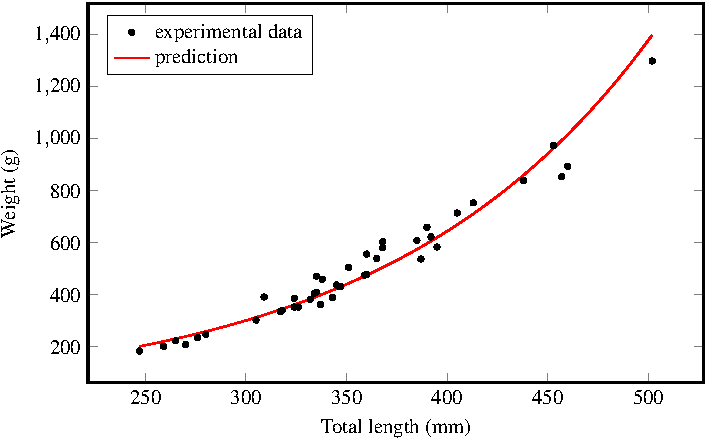
\includegraphics[scale=1.1]{image/12/rainbow-trout.pdf}
\caption{%%
  The total length versus weight of $42$ rainbow trout.  The
  experimental data are from \Table{tab:logarithm:rainbow_trout}.  The
  red curve is a graph of
  \Equation{eqn:logarithm:rainbow_trout_prediction}.
}
\label{fig:rainbow_trout_prediction}
\end{figure}

\solutionpart{subex:logarithm:trout_formula_graph}
Using the estimates
from \Part{subex:logarithm:trout_linear_regression}, if $Q(x)$
represents the weight~(g) of a rainbow trout that has a total length
of $x$~(mm), then $Q(x)$ can be written as
%%
\begin{equation}
\label{eqn:logarithm:rainbow_trout_prediction}
Q(x)
=
30.8338 \cdot e^{0.0076 x}.
\end{equation}
%%
\Figure{fig:rainbow_trout_prediction} shows a graph of
\Equation{eqn:logarithm:rainbow_trout_prediction} together with the
experimental data.
\end{solution}

\begin{exercise}
In \Example{ex:logarithm:rainbow_trout}, calculate the root mean
square error of
\Equation{eqn:logarithm:rainbow_trout_prediction} and the Pearson
correlation coefficient of the model.
\end{exercise}

\ifbool{showSolution}{
\begin{solution}
The root mean square error of
\Equation{eqn:logarithm:rainbow_trout_prediction} is $50.1968$,
rounded to four decimal places.  The model has a correlation
coefficient of $0.9792$, rounded to four decimal places.
\end{solution}
}{}

\begin{table}[!htbp]
\centering
\begin{tabular}{ccrrcc} \toprule
Time  & Count && Time   & Count \\\midrule
$0$   & $787$ && $603$  & $236$ \\
$30$  & $738$ && $633$  & $179$ \\
$60$  & $667$ && $663$  & $212$ \\
$90$  & $654$ && $693$  & $189$ \\
$121$ & $565$ && $723$  & $170$ \\
$151$ & $527$ && $753$  & $178$ \\
$181$ & $556$ && $784$  & $160$ \\
$211$ & $505$ && $814$  & $124$ \\
$241$ & $474$ && $844$  & $140$ \\
$271$ & $407$ && $874$  & $114$ \\
$302$ & $368$ && $904$  & $131$ \\
$332$ & $393$ && $934$  & $117$ \\
$362$ & $334$ && $964$  & $140$ \\
$392$ & $327$ && $995$  & $94$  \\
$422$ & $312$ && $1025$ & $107$ \\
$452$ & $293$ && $1055$ & $103$ \\
$482$ & $278$ && $1085$ & $94$  \\
$512$ & $249$ && $1115$ & $79$  \\
$543$ & $250$ && $1145$ & $94$  \\
$573$ & $238$ && $1175$ & $68$  \\\bottomrule
\end{tabular}

\caption{%%
  The radioactive decay of a sample of $9.7656$ grams of copper.  The
  sample was neutron activated for $66$ minutes.  Then a Geiger
  counter was used to measure the number of radioactive isotopes after
  the elapse of the listed number of seconds.  The experiment was
  performed by Steven Sahyun at the University of Wisconsin at
  Whitewater, USA on $13$-th January~$2005$.
}
\label{tab:logarithm:copper_radioactive_decay}
\end{table}

\begin{exercise}
\textbf{Radioactive decay of copper.}
\Table{tab:logarithm:copper_radioactive_decay} shows the radioactive
decay of a sample of copper.\footnote{
  The data set was available at:
  \url{http://web.archive.org/web/20180515171532/http://sahyun.net/physics/neutron/data/Cu_data_2.xls},
  accessed 2018-05-16.
}
The columns for ``Time'' list the elapsed time in seconds, while the
columns for ``Count'' list the corresponding number of radioactive
isotopes as measured by a Geiger counter.
%%
\begin{packedenum}
\item\label{subex:logarithm:copper_decay_linear_log_plots}
  Plot the data in the table by using a linear scale for both the
  horizontal and vertical axes.  What do you notice in the linear
  plot?  Now take the natural logarithm of each value in the ``Count''
  columns and produce a semi-log plot.  What do you notice in the
  semi-log plot?

\item\label{subex:logarithm:copper_decay_regression}
  Suppose that the data in
  \Table{tab:logarithm:copper_radioactive_decay} follow the
  exponential model $Q(x) = a \cdot e^{rx}$, whose logarithmic
  transformation is $\ln Q(x) = rx + \ln a$.  Use linear regression to
  estimate the parameters $r$ and $\ln a$.  Use the estimate for
  $\ln a$ to calculate an estimation of $a$.  Graph the model $Q(x)$
  together with the linear plot
  from \Part{subex:logarithm:copper_decay_linear_log_plots}.

\item\label{subex:logarithm:copper_decay_RMS_error_Pearson_rho}
  Calculate the root mean square~(RMS) error of your model $Q(x)$
  from \Part{subex:logarithm:copper_decay_regression}.  Determine the
  Pearson correlation coefficient $\rho$ of the model.  Provide an
  interpretation of the values of $\rho$ and the RMS error.
\end{packedenum}
\end{exercise}

\ifbool{showSolution}{
\begin{solution}
\solutionpart{subex:logarithm:copper_decay_linear_log_plots}
\Figure{subfig:logarithm:copper_decay_linear} shows a scatter plot of
the data in \Table{tab:logarithm:copper_radioactive_decay}, where the
horizontal and vertical axes use linear scaling.  The graph suggests
that the points roughly follow a model of exponential decay.
\Figure{subfig:logarithm:copper_decay_log} shows a semi-log plot of
the same data set, but with logarithmic scaling for the vertical
axis.  The graph shows that the points seem to lie around a straight
whose gradient is negative.  This further demonstrates that the data
set might be modelled as a function for exponential decay.

\begin{figure}[!htbp]
\centering
\subfigure[]{
  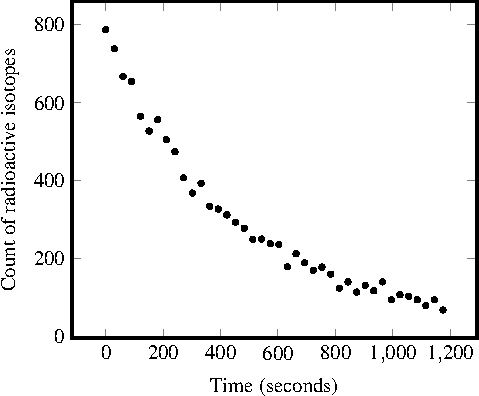
\includegraphics[scale=0.81]{image/12/copper-decay-linear.pdf}
  \label{subfig:logarithm:copper_decay_linear}
}
%%
%%
\subfigure[]{
  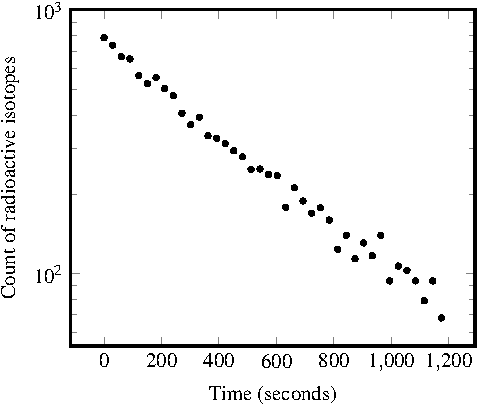
\includegraphics[scale=0.81]{image/12/copper-decay-log.pdf}
  \label{subfig:logarithm:copper_decay_log}
}
\caption{%%
  The radioactive decay of a sample of copper that had been neutron
  activated.  Data are from
  \Table{tab:logarithm:copper_radioactive_decay}.  (a)~A scatter plot
  of the time in seconds versus the count of radioactive isotopes with
  linear axes.  (b)~A semi-log plot of the same data set, where the
  vertical axis uses logarithmic scaling.
}
\label{fig:logarithm:copper_decay}
\end{figure}

\begin{table}[!htbp]
\centering
\begin{tabular}{rrrrrr} \toprule
$x$    & $y$      & $d(x_i)$   & $d(y_i)$  & $d(x_i)d(y_i)$ & $d(x_i)d(x_i)$ \\\midrule
$0$    & $6.6682$ & $-587.725$ & $1.2215$  & $-717.9189$   & $345420.6756$  \\
$30$   & $6.6039$ & $-557.725$ & $1.1572$  & $-645.4202$   & $311057.1756$  \\
$60$   & $6.5028$ & $-527.725$ & $1.0561$  & $-557.3217$   & $278493.6756$  \\
$90$   & $6.4831$ & $-497.725$ & $1.0364$  & $-515.8426$   & $247730.1756$  \\
$121$  & $6.3368$ & $-466.725$ & $0.8901$  & $-415.4409$   & $217832.2256$  \\
$151$  & $6.2672$ & $-436.725$ & $0.8205$  & $-358.3303$   & $190728.7256$  \\
$181$  & $6.3208$ & $-406.725$ & $0.8741$  & $-355.5028$   & $165425.2256$  \\
$211$  & $6.2246$ & $-376.725$ & $0.7779$  & $-293.0363$   & $141921.7256$  \\
$241$  & $6.1612$ & $-346.725$ & $0.7145$  & $-247.7353$   & $120218.2256$  \\
$271$  & $6.0088$ & $-316.725$ & $0.5621$  & $-178.0333$   & $100314.7256$  \\
$302$  & $5.9081$ & $-285.725$ & $0.4614$  & $-131.8268$   & $81638.7756$   \\
$332$  & $5.9738$ & $-255.725$ & $0.5271$  & $-134.7935$   & $65395.2756$   \\
$362$  & $5.8111$ & $-225.725$ & $0.3644$  & $-82.2620$    & $50951.7756$   \\
$392$  & $5.7900$ & $-195.725$ & $0.3433$  & $-67.1833$    & $38308.2756$   \\
$422$  & $5.7430$ & $-165.725$ & $0.2963$  & $-49.1038$    & $27464.7756$   \\
$452$  & $5.6802$ & $-135.725$ & $0.2335$  & $-31.6872$    & $18421.2756$   \\
$482$  & $5.6276$ & $-105.725$ & $0.1809$  & $-19.1272$    & $11177.7756$   \\
$512$  & $5.5175$ & $-75.725$  & $0.0707$  & $-5.3573$     & $5734.2756$    \\
$543$  & $5.5215$ & $-44.725$  & $0.0748$  & $-3.3434$     & $2000.3256$    \\
$573$  & $5.4723$ & $-14.725$  & $0.0256$  & $-0.3764$     & $216.8256$     \\
$603$  & $5.4638$ & $15.275$   & $0.0171$  & $0.2616$      & $233.3256$     \\
$633$  & $5.1874$ & $45.275$   & $-0.2593$ & $-11.7407$    & $2049.8256$    \\
$663$  & $5.3566$ & $75.275$   & $-0.0901$ & $-6.7838$     & $5666.3256$    \\
$693$  & $5.2417$ & $105.275$  & $-0.2050$ & $-21.5771$    & $11082.8256$   \\
$723$  & $5.1358$ & $135.275$  & $-0.3109$ & $-42.0581$    & $18299.3256$   \\
$753$  & $5.1818$ & $165.275$  & $-0.2649$ & $-43.7851$    & $27315.8256$   \\
$784$  & $5.0752$ & $196.275$  & $-0.3715$ & $-72.9226$    & $38523.8756$   \\
$814$  & $4.8203$ & $226.275$  & $-0.6264$ & $-141.7443$   & $51200.3756$   \\
$844$  & $4.9416$ & $256.275$  & $-0.5051$ & $-129.4353$   & $65676.8756$   \\
$874$  & $4.7362$ & $286.275$  & $-0.7105$ & $-203.4007$   & $81953.3756$   \\
$904$  & $4.8752$ & $316.275$  & $-0.5715$ & $-180.7541$   & $100029.8756$  \\
$934$  & $4.7622$ & $346.275$  & $-0.6845$ & $-237.0365$   & $119906.3756$  \\
$964$  & $4.9416$ & $376.275$  & $-0.5051$ & $-190.0430$   & $141582.8756$  \\
$995$  & $4.5433$ & $407.275$  & $-0.9034$ & $-367.9370$   & $165872.9256$  \\
$1025$ & $4.6728$ & $437.275$  & $-0.7739$ & $-338.3973$   & $191209.4256$  \\
$1055$ & $4.6347$ & $467.275$  & $-0.8120$ & $-379.4168$   & $218345.9256$  \\
$1085$ & $4.5433$ & $497.275$  & $-0.9034$ & $-449.2440$   & $247282.4256$  \\
$1115$ & $4.3694$ & $527.275$  & $-1.0773$ & $-568.0115$   & $278018.9256$  \\
$1145$ & $4.5433$ & $557.275$  & $-0.9034$ & $-503.4487$   & $310555.4256$  \\
$1175$ & $4.2195$ & $587.275$  & $-1.2272$ & $-720.7032$   & $344891.9256$  \\\bottomrule
\end{tabular}

\caption{%%
  Detailed calulation of the regression of the data in
  \Table{tab:logarithm:copper_radioactive_decay}.  The column with the
  heading $x$ lists the elapsed times in seconds.  The column with the
  heading $y$ lists the natural logarithm of the data in the ``Count''
  columns of \Table{tab:logarithm:copper_radioactive_decay}.  Let
  $\xbar$ and $\ybar$ be the means of the $x$ and $y$ columns,
  respectively.  Then $d(x_i) = x_i - \xbar$ and
  $d(y_i) = y_i - \ybar$.  Most numbers have been rounded to four
  decimal places so as to fit the table.  However, you should not
  round any intermediate results.
}
\label{tab:logarithm:copper_decay_regression}
\end{table}

\begin{figure}[!htbp]
\centering
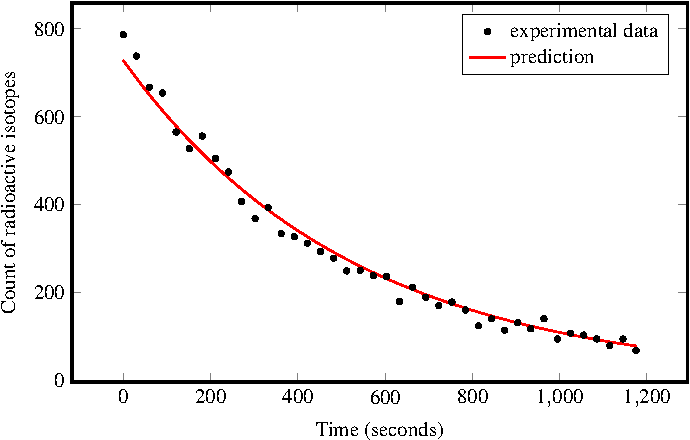
\includegraphics[scale=1.1]{image/12/copper-decay.pdf}
\caption{%%
  The radioactive decay of a sample of copper that had been neutron
  activated.  The black dots show the experimental data from
  \Table{tab:logarithm:copper_radioactive_decay} and the red curve is
  a graph of \Equation{eqn:logarithm:copper_decay_model}.
}
\label{fig:logarithm:copper_decay_data_versus_prediction}
\end{figure}

\solutionpart{subex:logarithm:copper_decay_regression}
\Table{tab:logarithm:copper_decay_regression} shows the detailed
calculation for the linear regression model
$\ln Q(x) = rx + \ln a$.  From the table, you have the sums
\[
\sum_{i=1}^n (x_i - \xbar) (y_i - \ybar)
\approx
-9417.8213
%%
\qquad
\text{and}
\qquad
%%
\sum_{i=1}^n (x_i - \xbar)^2
\approx
4840149.975
\]
where $n = 40$ is the number of data points in the table.  Then $r$
and $\ln a$ can be estimated as
\[
r
\approx
-0.0019
%%
\qquad
\text{and}
\qquad
%%
\ln a
\approx
6.5903
\]
and hence the parameter $a$ can be estimated as
$a \approx 727.9879$, with both $r$ and $a$ rounded to four decimal
places.  If $Q(x)$ represents the number of remaining radioactive
isotopes in the sample of copper after $x$ seconds, then the data in
\Table{tab:logarithm:copper_radioactive_decay} can be modelled as the
exponential decay function
%%
\begin{equation}
\label{eqn:logarithm:copper_decay_model}
Q(x)
=
727.9879 \cdot e^{-0.0019 x}.
\end{equation}
%%
\Figure{fig:logarithm:copper_decay_data_versus_prediction} shows a
graph of \Equation{eqn:logarithm:copper_decay_model} together with a
scatter plot of the data from
\Table{tab:logarithm:copper_radioactive_decay}.

\solutionpart{subex:logarithm:copper_decay_RMS_error_Pearson_rho}
The model in \Equation{eqn:logarithm:copper_decay_model} has a root
mean square~(RMS) error of $22.7376$, rounded to four decimal places.
Furthermore, the model has a Pearson correlation coefficient of
$\rho \approx -0.9924$, also rounded to four decimal places.  The low
values of the RMS error and $\rho$ suggest that
\Equation{eqn:logarithm:copper_decay_model} is a good fit of the
experimental data.
\end{solution}
}{}

\begin{exercise}
Use the data set at
\url{http://resources.seattlecentral.edu/qelp/sets/071/071.html}.
\end{exercise}

\ifbool{showSolution}{
\begin{solution}

\end{solution}
}{}


%%%%%%%%%%%%%%%%%%%%%%%%%%%%%%%%%%%%%%%%%%%%%%%%%%%%%%%%%%%%%%%%%%%%%%%%%%%

\subsection{Logarithmic scaling on horizontal axis}
\label{subsec:logarithm:logarithmic_scaling_on_horizontal_axis}

In some cases, a scatter plot of a data set might suggest that the
data follow a logarithmic function.  For instance,
\Table{tab:logarithm:hinoki_cypress} lists the age versus height of a
hinoki cypress tree.\footnote{
  The data set was published in the following paper:
  \url{https://doi.org/10.1093/treephys/tps127}.
  The data in the table are for the hinoki cypress tree to which the
  authors of the paper assigned the ID of ``Tree~1''.
}
The data set is illustrated as the scatter plot in
\Figure{fig:logarithm:hinoki_cypress_linear} with linear scaling for
both of the horizontal and vertical axes.  The figure seems to show
that the dots follow a logarithmic function, although it is possible
that the dots might follow a linear function.
\Figure{fig:logarithm:hinoki_cypress_log} shows a scatter plot of the
same data set, except that the horizontal axis now uses logarithmic
scaling.  The semi-log plot in
\Figure{fig:logarithm:hinoki_cypress_log} suggests that the dots
follow a straight line.  In other words, the scatter plots in
\Figure{fig:logarithm:hinoki_cypress} suggest that you might try to
model the data in \Table{tab:logarithm:hinoki_cypress} as a
logarithmic function.  But how?

\begin{table}[!htbp]
\centering
\begin{tabular}{ccrrcc} \toprule
Age  & Height &&& Age  & Height \\\midrule
$21$ & $6.90$ &&& $31$ & $8.25$ \\
$22$ & $7.65$ &&& $32$ & $8.74$ \\
$23$ & $7.67$ &&& $33$ & $8.87$ \\
$24$ & $7.76$ &&& $34$ & $8.91$ \\
$25$ & $7.99$ &&& $35$ & $8.96$ \\
$26$ & $7.85$ &&& $36$ & $9.01$ \\
$27$ & $7.96$ &&& $37$ & $9.05$ \\
$28$ & $7.99$ &&& $38$ & $9.07$ \\
$29$ & $8.50$ &&& $39$ & $9.04$ \\
$30$ & $8.46$ &&& $40$ & $9.12$ \\\bottomrule
\end{tabular}

\caption{%%
  The age of a hinoki cypress tree versus its height.  Age is measured
  in tree years and height is measured in metres.
}
\label{tab:logarithm:hinoki_cypress}
\end{table}

\begin{figure}[!htbp]
\centering
\subfigure[]{
  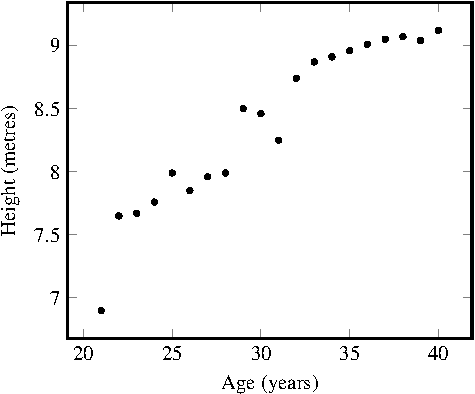
\includegraphics[scale=0.8]{image/12/hinoki-cypress-linear.pdf}
  \label{fig:logarithm:hinoki_cypress_linear}
}
%%
%%
\subfigure[]{
  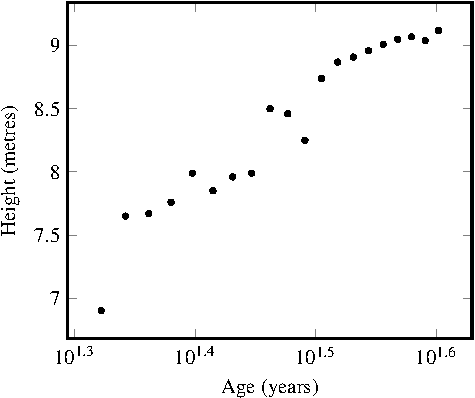
\includegraphics[scale=0.8]{image/12/hinoki-cypress-log.pdf}
  \label{fig:logarithm:hinoki_cypress_log}
}
\caption{%%
  The age~(in tree years) of a hinoki cypress versus its height~(in
  metres).  (a)~A scatter plot with linear scaling for both axes.
  (b)~A scatter plot of the same data set, but with logarithmic
  scaling for the horizontal axis.
}
\label{fig:logarithm:hinoki_cypress}
\end{figure}

If a data set follows a logarithmic function, how can you determine a
logarithmic function that best fits the data?  The first thing you
need to do is to be precise about which logarithmic function you think
the data follow.  Is it a natural logarithmic function?  A common
logarithmic function?  A logarithmic function with base $2$.  Or a
logarithmic function with some other base?  For now, suppose that your
data set can be modelled as the natural logarithmic function
%%
\begin{equation}
\label{eqn:logarithm:log_scaling_horizontal_axis}
Q(x)
=
a \cdot \ln x + b
\end{equation}
%%
where the parameters $a$ and $b$ are to be determined from the data.
The assumption is that you take the natural logarithm of the values in
the $x$ column; call this the natural logarithmic transformation of
the $x$ column.  In the case of \Table{tab:logarithm:hinoki_cypress},
the $x$ column is the column with the heading ``Age''.  You leave the
$y$~(i.e.~the ``Height'') column alone with its linear scaling.  Thus
you have linearised the data.  A scatter plot of the linearised data
should show a bunch of points that seem to follow a straight line; see
for example \Figure{fig:logarithm:hinoki_cypress_log}.  In that case,
the linear regression function of the linearised data is in fact of
the form shown in
\Equation{eqn:logarithm:log_scaling_horizontal_axis}.  Determine the
linear regression function of the linearised data and let the
parameters $\alphahat$ and $\betahat$ of the regression function be
estimates of $a$ and $b$, respectively.  The above technique is called
\emph{logarithmic regression} because you are fitting a logarithmic
function to a data set.  \Example{eg:logarithm:hinoki_cypress_tree}
below clarifies the technique.

\begin{table}[!htbp]
\centering
\begin{tabular}{cccrrrcc} \toprule
$t$  & $x$      & $y$    & $d(x_i)$  & $d(y_i)$  & $d(x_i)d(y_i)$ & $d(x_i)d(x_i)$ & $d(y_i)d(y_i)$ \\\midrule
$21$ & $3.0445$ & $6.90$ & $-0.3547$ & $-1.4875$ & $0.5277$      & $0.1258$       & $2.2127$ \\
$22$ & $3.0910$ & $7.65$ & $-0.3082$ & $-0.7375$ & $0.2273$      & $0.0950$       & $0.5439$ \\
$23$ & $3.1355$ & $7.67$ & $-0.2638$ & $-0.7175$ & $0.1892$      & $0.0696$       & $0.5148$ \\
$24$ & $3.1781$ & $7.76$ & $-0.2212$ & $-0.6275$ & $0.1388$      & $0.0489$       & $0.3938$ \\
$25$ & $3.2189$ & $7.99$ & $-0.1804$ & $-0.3975$ & $0.0717$      & $0.0325$       & $0.1580$ \\
$26$ & $3.2581$ & $7.85$ & $-0.1412$ & $-0.5375$ & $0.0759$      & $0.0199$       & $0.2889$ \\
$27$ & $3.2958$ & $7.96$ & $-0.1034$ & $-0.4275$ & $0.0442$      & $0.0107$       & $0.1828$ \\
$28$ & $3.3322$ & $7.99$ & $-0.0670$ & $-0.3975$ & $0.0267$      & $0.0045$       & $0.1580$ \\
$29$ & $3.3673$ & $8.50$ & $-0.0320$ & $0.1125$  & $-0.0036$     & $0.0010$       & $0.0127$ \\
$30$ & $3.4012$ & $8.46$ & $0.0019$  & $0.0725$  & $0.0001$      & $0.0000$       & $0.0053$ \\
$31$ & $3.4340$ & $8.25$ & $0.0347$  & $-0.1375$ & $-0.0048$     & $0.0012$       & $0.0189$ \\
$32$ & $3.4657$ & $8.74$ & $0.0665$  & $0.3525$  & $0.0234$      & $0.0044$       & $0.1243$ \\
$33$ & $3.4965$ & $8.87$ & $0.0973$  & $0.4825$  & $0.0469$      & $0.0095$       & $0.2328$ \\
$34$ & $3.5264$ & $8.91$ & $0.1271$  & $0.5225$  & $0.0664$      & $0.0162$       & $0.2730$ \\
$35$ & $3.5553$ & $8.96$ & $0.1561$  & $0.5725$  & $0.0894$      & $0.0244$       & $0.3278$ \\
$36$ & $3.5835$ & $9.01$ & $0.1843$  & $0.6225$  & $0.1147$      & $0.0340$       & $0.3875$ \\
$37$ & $3.6109$ & $9.05$ & $0.2117$  & $0.6625$  & $0.1402$      & $0.0448$       & $0.4389$ \\
$38$ & $3.6376$ & $9.07$ & $0.2383$  & $0.6825$  & $0.1627$      & $0.0568$       & $0.4658$ \\
$39$ & $3.6636$ & $9.04$ & $0.2643$  & $0.6525$  & $0.1725$      & $0.0699$       & $0.4258$ \\
$40$ & $3.6889$ & $9.12$ & $0.2896$  & $0.7325$  & $0.2122$      & $0.0839$       & $0.5366$ \\\bottomrule
\end{tabular}

\caption{%%
  Detailed calculations of the logarithmic regression of the hinoki
  cypress data in \Table{tab:logarithm:hinoki_cypress}.  The tree age
  column $t$ and the tree height column $y$ are the same as the
  columns in \Table{tab:logarithm:hinoki_cypress}.  Each value in the
  $x$ column is the natural logarithmic transformation of the
  corresponding value in the age column $t$, i.e.~$x_i = \ln t_i$.  If
  $\xbar$ and $\ybar$ are the means of the $x$ and $y$ columns,
  respectively, then $d(x_i) = x_i - \xbar$ and
  $d(y_i) = y_i - \ybar$.  Most values in the table have been rounded
  to four decimal places in order to fit the table.  However, you
  should not round these intermediate results when you do your own
  calculations.
}
\label{tab:logarithm:hinoki_cypress_logarithmic_regression}
\end{table}

\begin{figure}[!htbp]
\centering
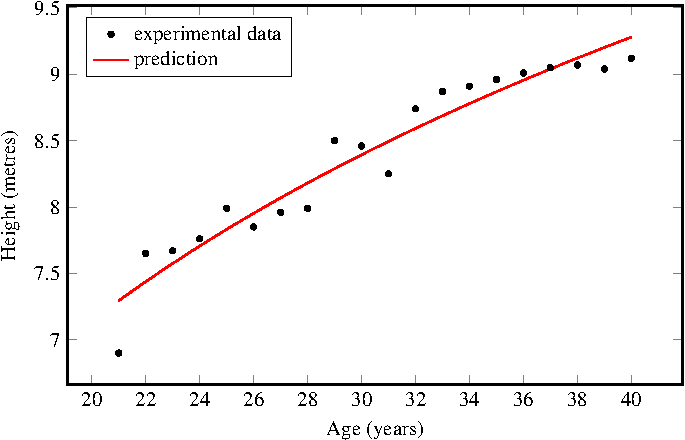
\includegraphics[scale=1.1]{image/12/hinoki-cypress.pdf}
\caption{%%
  The height in metres of a hinoki cypress tree as a function of its
  age in years.  The black dots show the experimental data from
  \Table{tab:logarithm:hinoki_cypress}.  The red curve is a graph of
  \Equation{eqn:logarithm:hinoki_cypress_log_regression}.
}
\label{fig:logarithm:hinoki_cypress_prediction}
\end{figure}

\begin{example}
\label{eg:logarithm:hinoki_cypress_tree}
\textbf{Hinoki cypress tree.}
Consider the data in \Table{tab:logarithm:hinoki_cypress}.
%%
\begin{packedenum}
\item\label{subex:logarithm:hinoki_cypress_log_transformation}
  Take the natural logarithm of each value in the ``Age'' column.

\item\label{subex:logarithm:hinoki_cypress_log_regression}
  Suppose that the data in \Table{tab:logarithm:hinoki_cypress} follow
  the natural logarithmic function $H(t) = a \ln t + b$, where $H(t)$
  represents the height in metres of a hinoki cypress tree at $t$
  years old.  Use linear regression to estimate the parameters $a$ and
  $b$.  Graph the function $H(t)$ together with the scatter plot in
  \Figure{fig:logarithm:hinoki_cypress_linear}.

\item\label{subex:logarithm:hinoki_cypress_correlation_r_RMS_error}
  Calculate the Pearson correlation coefficient $\rho$ of the model
  $H(t)$ from \Part{subex:logarithm:hinoki_cypress_log_regression} and
  the root mean square~(RMS) error of the model.  Provide an
  interpretation of the values of $\rho$ and the RMS error.
\end{packedenum}
\end{example}

\begin{solution}
\solutionpart{subex:logarithm:hinoki_cypress_log_transformation}
See the $x$ column in
\Table{tab:logarithm:hinoki_cypress_logarithmic_regression}.

\solutionpart{subex:logarithm:hinoki_cypress_log_regression}
First, you should linearise the data in
\Table{tab:logarithm:hinoki_cypress}, which you have done
in \Part{subex:logarithm:hinoki_cypress_log_transformation} by taking
the natural logarithm of each value in the ``Age'' column.  The result
is the $x$ column in
\Table{tab:logarithm:hinoki_cypress_logarithmic_regression}.

Second, you perform linear regression on the $x$ and $y$ columns of
\Table{tab:logarithm:hinoki_cypress_logarithmic_regression}.  Results
of the regression include the numbers $\alpha$ and $\beta$, which you
treat as estimates of the parameters $a$ and $b$, respectively.  The
means of the $x$ and $y$ columns are $\xbar \approx 3.3993$ and
$\ybar \approx 8.3875$, both rounded to four decimal places.
\Table{tab:logarithm:hinoki_cypress_logarithmic_regression} shows the
detailed calculations of the linear regression, from which you obtain
the sums
\[
\sum_{i=1}^n (x_i - \xbar) (y_i - \ybar)
\approx
2.3216
%%
\qquad
\text{and}
\qquad
%%
\sum_{i=1}^n (x_i - \xbar)^2
\approx
0.7529
\]
rounded to four decimal places, where $n = 20$ is the number of data
points in \Table{tab:logarithm:hinoki_cypress}.  Then you have the
numbers
%%
\begin{align*}
\alpha
&=
\frac{
  \sum_{i=1}^n (x_i - \xbar) (y_i - \ybar)
}{
  \sum_{i=1}^n (x_i - \xbar)^2
}
\approx
3.0835 \\[4pt]
%%
%%
\beta
&=
\ybar - \alpha\xbar
\approx
-2.0940
\end{align*}
%%
both rounded to four decimal places.  Consider these two numbers as
estimates of the parameters $a$ and $b$.  Hence the height $H(t)$ of
the hinoki cypress tree at $t$ years old can be modelled as
%%
\begin{equation}
\label{eqn:logarithm:hinoki_cypress_log_regression}
H(t)
=
3.0835 \ln t - 2.0940.
\end{equation}
%%
\Figure{fig:logarithm:hinoki_cypress_prediction} shows a graph of the
model~\eqref{eqn:logarithm:hinoki_cypress_log_regression} together
with a scatter plot of the data in
\Table{tab:logarithm:hinoki_cypress}.

\solutionpart{subex:logarithm:hinoki_cypress_correlation_r_RMS_error}
The model~\eqref{eqn:logarithm:hinoki_cypress_log_regression} has a
Pearson correlation coefficient of $\rho \approx 0.9641$ and a root
mean square~(RMS) error of approximately $0.1649$, both numbers
rounded to four decimal places.  The high value of $\rho$ and the low
value of the RMS error both suggest that
\Equation{eqn:logarithm:hinoki_cypress_log_regression} provide a good
fit of the data in \Table{tab:logarithm:hinoki_cypress}.
\end{solution}

\begin{exercise}
\textbf{Hinoki cypress tree.}
In \Example{eg:logarithm:hinoki_cypress_tree},
\Figure{fig:logarithm:hinoki_cypress_linear} shows that the data in
\Table{tab:logarithm:hinoki_cypress} seems to follow a straight line.
Assume that the experimental data follow a linear function of the form
$f(x) = ax + b$, where $f(x)$ represents the height of the hinoki
cypress tree at $x$ years of age.
%%
\begin{packedenum}
\item\label{subex:logarithm:hinoki_linear_regression}
  Use linear regression to estimate the parameters $a$ and $b$.  Graph
  the model $f(x)$ together with the graph in
  \Figure{fig:logarithm:hinoki_cypress_prediction}.

\item\label{subex:logarithm:hinoki_Pearson_rho_RMS_error}
  Calculate the Pearson correlation coefficient $\rho$ of the model
  $f(x)$ and the root mean square~(RMS) error of the model.  Use these
  values, and the values of $\rho$ and the RMS error from
  \Example{eg:logarithm:hinoki_cypress_tree}, to help you determine
  which one of the functions $f(x)$ and $H(t)$ is better than the
  other at modelling the data in
  \Table{tab:logarithm:hinoki_cypress}.
\end{packedenum}
\end{exercise}

\ifbool{showSolution}{
\begin{solution}
\solutionpart{subex:logarithm:hinoki_linear_regression}
\Table{tab:logarithm:hinoki_cypress_linear_regression} shows the
detailed calculations for the linear regression of the data in
\Table{tab:logarithm:hinoki_cypress}.  The means of the $x$ and $y$
columns are $\xbar = 30.5$ and $\ybar = 8.3875$, respectively.  Use
the values in \Table{tab:logarithm:hinoki_cypress_linear_regression}
to obtain the sums
\[
\sum_{i=1}^n (x_i - \xbar) (y_i - \ybar)
\approx
68.1750
%%
\qquad
\text{and}
\qquad
%%
\sum_{i=1}^n (x_i - \xbar)^2
=
665
\]
where $n = 20$ is the number of data points.  Then the parameters $a$
and $b$ can be estimated as $a \approx 0.1025$ and $b \approx 5.2607$,
respectively, both numbers rounded to four decimal places.  The data
in \Table{tab:logarithm:hinoki_cypress} can now be modelled as
%%
\begin{equation}
\label{eqn:logarithm:hinoki_cypress_linear_regression}
f(x)
=
0.1025x + 5.2607.
\end{equation}
%%
\Figure{fig:logarithm:hinoki_cypress_regression_comparison} compares
\Equations{eqn:logarithm:hinoki_cypress_log_regression}{eqn:logarithm:hinoki_cypress_linear_regression}
together with the data in \Table{tab:logarithm:hinoki_cypress}.

\begin{table}[!htbp]
\centering
\begin{tabular}{ccrrrrc} \toprule
$x$  & $y$    & $d(x_i)$ & $d(y_i)$  & $d(x_i)d(y_i)$ & $d(x_i)d(x_i)$ & $d(y_i)d(y_i)$ \\\midrule
$21$ & $6.90$ & $-9.5$   & $-1.4875$ & $14.1313$      & $90.25$       & $2.2127$ \\
$22$ & $7.65$ & $-8.5$   & $-0.7375$ & $6.2687$       & $72.25$       & $0.5439$ \\
$23$ & $7.67$ & $-7.5$   & $-0.7175$ & $5.3813$       & $56.25$       & $0.5148$ \\
$24$ & $7.76$ & $-6.5$   & $-0.6275$ & $4.0788$       & $42.25$       & $0.3938$ \\
$25$ & $7.99$ & $-5.5$   & $-0.3975$ & $2.1863$       & $30.25$       & $0.1580$ \\
$26$ & $7.85$ & $-4.5$   & $-0.5375$ & $2.4188$       & $20.25$       & $0.2889$ \\
$27$ & $7.96$ & $-3.5$   & $-0.4275$ & $1.4963$       & $12.25$       & $0.1828$ \\
$28$ & $7.99$ & $-2.5$   & $-0.3975$ & $0.9937$       & $6.25$        & $0.1580$ \\
$29$ & $8.50$ & $-1.5$   & $0.1125$  & $-0.1688$      & $2.25$        & $0.0127$ \\
$30$ & $8.46$ & $-0.5$   & $0.0725$  & $-0.0363$      & $0.25$        & $0.0053$ \\
$31$ & $8.25$ & $0.5$    & $-0.1375$ & $-0.0687$      & $0.25$        & $0.0189$ \\
$32$ & $8.74$ & $1.5$    & $0.3525$  & $0.5288$       & $2.25$        & $0.1243$ \\
$33$ & $8.87$ & $2.5$    & $0.4825$  & $1.2063$       & $6.25$        & $0.2328$ \\
$34$ & $8.91$ & $3.5$    & $0.5225$  & $1.8288$       & $12.25$       & $0.2730$ \\
$35$ & $8.96$ & $4.5$    & $0.5725$  & $2.5763$       & $20.25$       & $0.3278$ \\
$36$ & $9.01$ & $5.5$    & $0.6225$  & $3.4238$       & $30.25$       & $0.3875$ \\
$37$ & $9.05$ & $6.5$    & $0.6625$  & $4.3063$       & $42.25$       & $0.4389$ \\
$38$ & $9.07$ & $7.5$    & $0.6825$  & $5.1188$       & $56.25$       & $0.4658$ \\
$39$ & $9.04$ & $8.5$    & $0.6525$  & $5.5463$       & $72.25$       & $0.4258$ \\
$40$ & $9.12$ & $9.5$    & $0.7325$  & $6.9588$       & $90.25$       & $0.5366$ \\\bottomrule
\end{tabular}

\caption{%%
  Detailed calculations of the linear regression of the hinoki cypress
  data in \Table{tab:logarithm:hinoki_cypress}.  Note that the $x$ and
  $y$ columns are the same as the ``Age'' and ``Height'' columns in
  \Table{tab:logarithm:hinoki_cypress}.  If $\xbar$ and $\ybar$ are
  the means of the $x$ and $y$ columns, respectively, then
  $d(x_i) = x_i - \xbar$ and $d(y_i) = y_i - \ybar$.  Most values in
  the table have been rounded to four decimal places in order to fit
  the table.  However, you should not round these intermediate results
  when you perform your own calculations.
}
\label{tab:logarithm:hinoki_cypress_linear_regression}
\end{table}

\begin{figure}[!htbp]
\centering
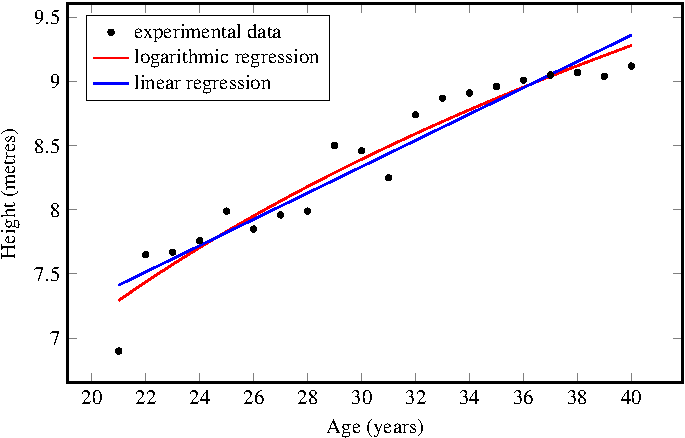
\includegraphics[scale=1.1]{image/12/hinoki-cypress-linear-log.pdf}
\caption{%%
  A comparison of the logarithmic regression
  function~\eqref{eqn:logarithm:hinoki_cypress_log_regression} and the
  linear regression
  function~\eqref{eqn:logarithm:hinoki_cypress_linear_regression}.
  The black dots show the data from
  \Table{tab:logarithm:hinoki_cypress}.
}
\label{fig:logarithm:hinoki_cypress_regression_comparison}
\end{figure}

\solutionpart{subex:logarithm:hinoki_Pearson_rho_RMS_error}
The model~\eqref{eqn:logarithm:hinoki_cypress_linear_regression} has a
Pearson correlation coefficient of $\rho \approx 0.9526$ and a root
mean square~(RMS) error of $0.1888$, both numbers rounded to four
decimal places.  The $\rho$ value of
\Equation{eqn:logarithm:hinoki_cypress_linear_regression} is smaller
than the $\rho$ value of the logarithmic regression from
\Example{eg:logarithm:hinoki_cypress_tree}.  Furthermore, the RMS
error of \Equation{eqn:logarithm:hinoki_cypress_linear_regression} is
higher than the RMS error of
\Equation{eqn:logarithm:hinoki_cypress_log_regression}.  Conclude that
\Equation{eqn:logarithm:hinoki_cypress_log_regression} is better than
\Equation{eqn:logarithm:hinoki_cypress_linear_regression} at modelling
the hinoki cypress data set.
\end{solution}
}{}

\begin{table}[!htbp]
\centering
\begin{tabular}{ccrrcc} \toprule
Mean DBH & Mean height &&& Mean DBH & Mean height \\\midrule
$16.19$  & $8.60$      &&& $23.47$  & $12.22$ \\
$31.45$  & $16.40$     &&& $19.00$  & $10.55$ \\
$14.17$  & $9.10$      &&& $17.32$  & $10.15$ \\
$14.68$  & $7.80$      &&& $20.92$  & $10.73$ \\
$20.88$  & $12.49$     &&& $17.68$  & $9.50$  \\
$49.34$  & $21.33$     &&& $21.76$  & $12.89$ \\
$17.63$  & $11.31$     &&& $22.31$  & $13.00$ \\
$15.58$  & $10.40$     &&& $24.00$  & $14.62$ \\
$32.03$  & $14.30$     &&& $35.18$  & $16.71$ \\
$20.34$  & $12.08$     &&& $33.04$  & $15.72$ \\
$22.88$  & $14.83$     &&& $24.14$  & $14.37$ \\
$13.24$  & $7.70$      &&& $27.41$  & $13.94$ \\
$29.62$  & $16.30$     &&& $18.13$  & $10.22$ \\
$48.07$  & $17.78$     &&& $19.61$  & $11.79$ \\
$17.27$  & $10.75$     &&& $46.88$  & $22.72$ \\
$26.27$  & $15.93$     &&& $21.45$  & $11.74$ \\
$23.17$  & $11.83$     &&& $21.07$  & $9.30$  \\
$26.44$  & $15.59$ \\\bottomrule
\end{tabular}

\caption{%%
  The mean diameter at breast height~(DBH) versus mean height of $35$
  species of trees in a selective logging forest.  The study site was
  called Sombo and the forest was located in the northern region of
  the Republic of Congo, Africa.  The DBH of a tree is usually
  measured at $1.3$ metres above ground level.  DBH is measured in
  centimetres and tree height is measured in metres.
}
\label{tab:logarithm:Sombo}
\end{table}

\begin{exercise}
\Table{tab:logarithm:Sombo} shows the mean diameter at breast
height~(cm) versus the mean height~(m) of $35$ species of trees in a
northern region of the Republic of Congo, Africa.\footnote{
  The data set was published in the paper:
  \url{https://doi.org/10.4236/oje.2018.83014}.
}
%%
\begin{packedenum}
\item\label{subex:logarithm:Sombo_graph_linear_log}
  Produce two graphs of the data in \Table{tab:logarithm:Sombo}.  One
  graph is a scatter plot that uses linear scaling for both of the
  horizontal and vertical axes.  The other graph is the same scatter
  plot, but with logarithmic scaling on the horizontal axis.  What do
  you notice about the two graphs?

\item\label{subex:logarithm:Sombo_log_regression}
  Suppose that the data in \Table{tab:logarithm:Sombo} follow a
  logarithmic function of the form $H(x) = a \ln x + b$, where $H(x)$
  represents the mean height~(in metres) of a species of tree that
  have a mean DBH of $x$ centimetres.  Use logarithmic regression to
  estimate the parameters $a$ and $b$.  Graph the function $H(x)$
  together with a scatter plot of the data in
  \Table{tab:logarithm:Sombo}.  Use linear scaling for both of the
  horizontal and vertical axes.  Calculate the Pearson correlation
  coefficient of the model $H(x)$ and the root mean square error of
  the model.

\item\label{subex:logarithm:Sombo_linear_regression}
  Suppose that the data in \Table{tab:logarithm:Sombo} follow a
  linear function of the form $f(x) = ax + b$, where $f(x)$ denotes
  the mean height~(in metres) of a species of tree that have a mean
  DBH of $x$ centimetres.  Use linear regression to estimate the
  parameters $a$ and $b$.  Graph the function $f(x)$ together with the
  graph from \Part{subex:logarithm:Sombo_log_regression}.  Calculate
  the Pearson correlation coefficient and root mean square~(RMS) error
  of the model.  Use the correlation coefficients and RMS errors to
  help you determine which one of the functions $f(x)$ and $H(x)$ is
  better suited to modelling the data in \Table{tab:logarithm:Sombo}.
\end{packedenum}
\end{exercise}

\ifbool{showSolution}{
\begin{solution}
\solutionpart{subex:logarithm:Sombo_graph_linear_log}
\Figure{subfig:logarithm:sombo_linear} shows a scatter plot of the
data in \Table{tab:logarithm:Sombo} with linear scaling for both of
the horizontal and vertical axes.  The graph shows that the points
seem to follow a logarithmic function.
\Figure{subfig:logarithm:sombo_log} shows the same scatter plot, but
using logarithmic scaling for the horizontal axis.  The graph suggests
that the points follow a straight line.

\begin{figure}[!htbp]
\centering
\subfigure[]{
  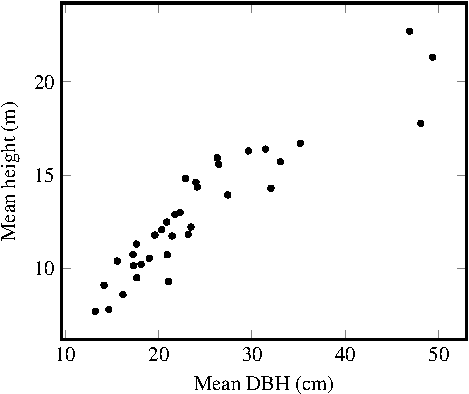
\includegraphics[scale=0.8]{image/12/sombo-linear.pdf}
  \label{subfig:logarithm:sombo_linear}
}
%%
%%
\subfigure[]{
  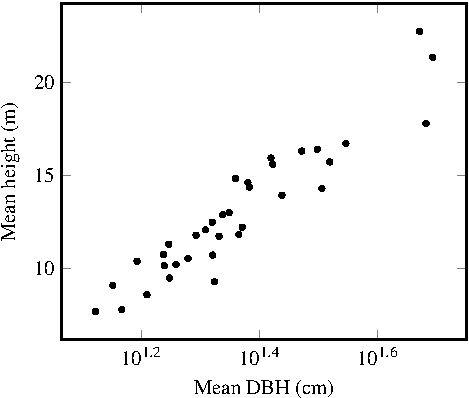
\includegraphics[scale=0.8]{image/12/sombo-log.pdf}
  \label{subfig:logarithm:sombo_log}
}
\caption{%%
  The mean diameter at breast height~(DBH) versus the mean height of
  $35$ species of trees.  The data are from
  \Table{tab:logarithm:Sombo}.  (a)~A scatter plot with linear scaling
  for both of the horizontal and vertical axes.  (b)~The same graph,
  but with logarithmic scaling for the horizontal axis.
}
\label{fig:logarithm:sombo}
\end{figure}

\begin{table}[!htbp]
\centering
\begin{tabular}{ccrrrrcr} \toprule
$x$     & $w$      & $y$     & $d(w_i)$  & $d(y_i)$  & $d(w_i)d(y_i)$ & $d(w_i)d(w_i)$ & $d(y_i)d(y_i)$ \\\midrule
$16.19$ & $2.7844$ & $8.60$  & $-0.3507$ & $-4.3911$ & $1.5400$      & $0.1230$       & $19.2821$ \\
$31.45$ & $3.4484$ & $16.40$ & $0.3133$  & $3.4089$  & $1.0680$      & $0.0982$       & $11.6203$ \\
$14.17$ & $2.6511$ & $9.10$  & $-0.4840$ & $-3.8911$ & $1.8832$      & $0.2342$       & $15.1410$ \\
$14.68$ & $2.6865$ & $7.80$  & $-0.4486$ & $-5.1911$ & $2.3288$      & $0.2013$       & $26.9480$ \\
$20.88$ & $3.0388$ & $12.49$ & $-0.0963$ & $-0.5011$ & $0.0483$      & $0.0093$       & $0.2511$  \\
$49.34$ & $3.8987$ & $21.33$ & $0.7636$  & $8.3389$  & $6.3678$      & $0.5831$       & $69.5365$ \\
$17.63$ & $2.8696$ & $11.31$ & $-0.2655$ & $-1.6811$ & $0.4463$      & $0.0705$       & $2.8262$  \\
$15.58$ & $2.7460$ & $10.40$ & $-0.3891$ & $-2.5911$ & $1.0083$      & $0.1514$       & $6.7140$  \\
$32.03$ & $3.4667$ & $14.30$ & $0.3316$  & $1.3089$  & $0.4340$      & $0.1099$       & $1.7131$  \\
$20.34$ & $3.0126$ & $12.08$ & $-0.1225$ & $-0.9111$ & $0.1116$      & $0.0150$       & $0.8302$  \\
$22.88$ & $3.1303$ & $14.83$ & $-0.0048$ & $1.8389$  & $-0.0089$     & $0.0000$       & $3.3814$  \\
$13.24$ & $2.5832$ & $7.70$  & $-0.5519$ & $-5.2911$ & $2.9200$      & $0.3046$       & $27.9962$ \\
$29.62$ & $3.3884$ & $16.30$ & $0.2533$  & $3.3089$  & $0.8383$      & $0.0642$       & $10.9485$ \\
$48.07$ & $3.8727$ & $17.78$ & $0.7376$  & $4.7889$  & $3.5320$      & $0.5440$       & $22.9332$ \\
$17.27$ & $2.8490$ & $10.75$ & $-0.2861$ & $-2.2411$ & $0.6413$      & $0.0819$       & $5.0227$  \\
$26.27$ & $3.2684$ & $15.93$ & $0.1333$  & $2.9389$  & $0.3918$      & $0.0178$       & $8.6369$  \\
$23.17$ & $3.1429$ & $11.83$ & $0.0078$  & $-1.1611$ & $-0.0090$     & $0.0001$       & $1.3483$  \\
$26.44$ & $3.2749$ & $15.59$ & $0.1398$  & $2.5989$  & $0.3633$      & $0.0195$       & $6.7541$  \\
$23.47$ & $3.1557$ & $12.22$ & $0.0206$  & $-0.7711$ & $-0.0159$     & $0.0004$       & $0.5947$  \\
$19.00$ & $2.9444$ & $10.55$ & $-0.1907$ & $-2.4411$ & $0.4654$      & $0.0364$       & $5.9592$  \\
$17.32$ & $2.8519$ & $10.15$ & $-0.2832$ & $-2.8411$ & $0.8047$      & $0.0802$       & $8.0721$  \\
$20.92$ & $3.0407$ & $10.73$ & $-0.0944$ & $-2.2611$ & $0.2134$      & $0.0089$       & $5.1128$  \\
$17.68$ & $2.8724$ & $9.50$  & $-0.2627$ & $-3.4911$ & $0.9170$      & $0.0690$       & $12.1881$ \\
$21.76$ & $3.0801$ & $12.89$ & $-0.0550$ & $-0.1011$ & $0.0056$      & $0.0030$       & $0.0102$  \\
$22.31$ & $3.1050$ & $13.00$ & $-0.0301$ & $0.0089$  & $-0.0003$     & $0.0009$       & $0.0001$  \\
$24.00$ & $3.1781$ & $14.62$ & $0.0430$  & $1.6289$  & $0.0700$      & $0.0018$       & $2.6532$  \\
$35.18$ & $3.5605$ & $16.71$ & $0.4254$  & $3.7189$  & $1.5819$      & $0.1809$       & $13.8299$ \\
$33.04$ & $3.4977$ & $15.72$ & $0.3626$  & $2.7289$  & $0.9895$      & $0.1315$       & $7.4467$  \\
$24.14$ & $3.1839$ & $14.37$ & $0.0488$  & $1.3789$  & $0.0672$      & $0.0024$       & $1.9012$  \\
$27.41$ & $3.3109$ & $13.94$ & $0.1758$  & $0.9489$  & $0.1668$      & $0.0309$       & $0.9003$  \\
$18.13$ & $2.8976$ & $10.22$ & $-0.2375$ & $-2.7711$ & $0.6582$      & $0.0564$       & $7.6792$  \\
$19.61$ & $2.9760$ & $11.79$ & $-0.1591$ & $-1.2011$ & $0.1911$      & $0.0253$       & $1.4427$  \\
$46.88$ & $3.8476$ & $22.72$ & $0.7125$  & $9.7289$  & $6.9317$      & $0.5076$       & $94.6507$ \\
$21.45$ & $3.0657$ & $11.74$ & $-0.0694$ & $-1.2511$ & $0.0868$      & $0.0048$       & $1.5654$  \\
$21.07$ & $3.0479$ & $9.30$  & $-0.0873$ & $-3.6911$ & $0.3221$      & $0.0076$       & $13.6245$ \\\bottomrule
\end{tabular}

\caption{%%
  Detailed calculations of the logarithmic regression of the data in
  \Table{tab:logarithm:Sombo}.  The $x$ and $y$ columns are the same
  as the ``Mean DBH'' and ``Mean height'' columns of
  \Table{tab:logarithm:Sombo}.  Each value in the $w$ column is the
  natural logarithmic transformation of the corresponding value in the
  $x$ column, i.e.~$w_i = \ln x_i$.  If $\wbar$ and $\ybar$ are the
  means of the $w$ and $y$ columns, respectively, then
  $d(w_i) = w_i - \wbar$ and $d(y_i) = y_i - \ybar$.  Most values in
  the table have been rounded to four decimal places so as to fit the
  table.  However, you should not round these intermediate results
  when you do your own calculations.
}
\label{tab:logarithm:Sombo_log_regression}
\end{table}

\solutionpart{subex:logarithm:Sombo_log_regression}
To perform a logarithmic regression of the data in
\Table{tab:logarithm:Sombo}, first you must take the natural logarithm
of each value in the ``Mean DBH'' columns.  The result is shown as the
$w$ column of \Table{tab:logarithm:Sombo_log_regression}, where the
$y$ column is the same as the ``Mean height'' columns of
\Table{tab:logarithm:Sombo}.  Second, you perform linear regression on
the $w$ and $y$ columns and let the estimates for $\alphahat$ and
$\betahat$ be estimates of $a$ and $b$, respectively.
\Table{tab:logarithm:Sombo_log_regression} shows the detailed
calculations of the logarithmic regression, where you have the means
$\wbar \approx 3.1351$ and $\ybar \approx 12.9911$, both numbers
rounded to four decimal places.  From the table, you obtain the sums
\[
\sum_{i=1}^n (w_i - \wbar) (y_i - \ybar)
\approx
37.3604
%%
\qquad
\text{and}
\qquad
%%
\sum_{i=1}^n (w_i - \wbar)^2
\approx
3.7761
\]
and the estimates
%%
\begin{align*}
\alphahat
&=
\frac{
  \sum_{i=1}^n (w_i - \wbar) (y_i - \ybar)
}{
  \sum_{i=1}^n (w_i - \wbar)^2
}
\approx
9.8940 \\[4pt]
%%
%%
\betahat
&=
\ybar - \alphahat \wbar
\approx
-18.0274
\end{align*}
%%
where $n = 35$ is the number of data points in
\Table{tab:logarithm:Sombo}, all numbers rounded to four decimal
places.  Hence you have the parameter estimations
$a \approx 9.8940$ and $b \approx -18.0274$ so that the data in
\Table{tab:logarithm:Sombo} can be modelled as
%%
\begin{equation}
\label{eqn:logarithm:Sombo_log_regression}
H(x)
=
9.8940 \ln x - 18.0274.
\end{equation}
%%
\Figure{fig:logarithm:Sombo_log_regression} compares
\Equation{eqn:logarithm:Sombo_log_regression} with the data in
\Table{tab:logarithm:Sombo}.  The model has a Pearson correlation
coefficient of $\rho \approx 0.9387$ and a root mean square error of
approximately $1.1937$, both numbers rounded to four decimal places.

\begin{figure}[!htbp]
\centering
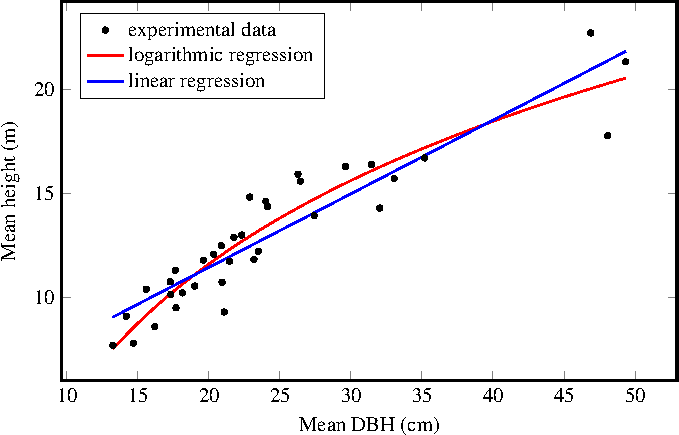
\includegraphics[scale=1.1]{image/12/sombo.pdf}
\caption{%%
  A comparison of experimental data versus predictions.  The black
  dots show the data points from \Table{tab:logarithm:Sombo}.  The red
  curve is a graph of the logarithmic regression
  function~\eqref{eqn:logarithm:Sombo_log_regression}.  The blue
  straight line is a graph of
  \Equation{eqn:logarithm:Sombo_linear_regression}.
}
\label{fig:logarithm:Sombo_log_regression}
\end{figure}

\solutionpart{subex:logarithm:Sombo_linear_regression}
A linear regression of the data in \Table{tab:logarithm:Sombo} shows
that the data can be modelled as
%%
\begin{equation}
\label{eqn:logarithm:Sombo_linear_regression}
f(x)
=
0.3539 x + 4.3699
\end{equation}
%%
where $f(x)$ represents the mean height~(m) of a species of tree that
have a mean DBH of $x$ centimetres.  The parameters have been rounded
to four decimal places.
Equation~\eqref{eqn:logarithm:Sombo_linear_regression} is graphed in
\Figure{fig:logarithm:Sombo_log_regression} together with
\Equation{eqn:logarithm:Sombo_log_regression} and the experimental
data in \Table{tab:logarithm:Sombo}.  The linear regression function
$f(x)$ has a Pearson correlation coefficient of $\rho \approx 0.9240$,
which is lower than the corresponding value for the logarithmic
regression function $H(x)$.  Furthermore, $f(x)$ has a root mean
square~(RMS) error of $1.3241$, which is higher than the RMS error of
$H(x)$.  Therefore you may conclude that
\Equation{eqn:logarithm:Sombo_log_regression} is better than
\Equation{eqn:logarithm:Sombo_linear_regression} at modelling the data
in \Table{tab:logarithm:Sombo}.
\end{solution}
}{}


%%%%%%%%%%%%%%%%%%%%%%%%%%%%%%%%%%%%%%%%%%%%%%%%%%%%%%%%%%%%%%%%%%%%%%%%%%%

\subsection{Logarithmic scaling on both axes}

In some cases, you need to use logarithmic scaling for both of the
horizontal and vertical axes.  As an example,
\Figure{fig:logarithm:Fortune100} shows two scatter plots of the same
data set on the number of employees and revenue of the top $100$
companies in the USA.\footnote{
  The data set was available at:
  \url{http://fortune.com/fortune500/list/},
  accessed 2018-05-13.
}
The scatter plot in \Figure{fig:logarithm:Fortune100_linear} has the
usual linear scale for the horizontal and vertical axes, which in its
present form shows a cluster of points in the lower-left corner and
one point in the upper-right corner.  What about the spacing of the
points in the cluster?  Suppose you take the common logarithm of each
number on the horizontal and vertical axes.  The result is the scatter
plot in \Figure{fig:logarithm:Fortune100_log}, which clearly shows the
spacing of the points in terms of multiples of $10$.  The graph in
\Figure{fig:logarithm:Fortune100_log} is called a \emph{log-log} plot
because numbers on both the horizontal and vertical axes have been
transformed to their equivalents under the common logarithm.  The
points in the log-log plot of \Figure{fig:logarithm:Fortune100_log} do
not seem to follow a straight, hence it is unlikely that a logarithmic
regression of the data would produce a high value of the Pearson
correlation coefficient.

\begin{figure}[!htbp]
\centering
\subfigure[]{
  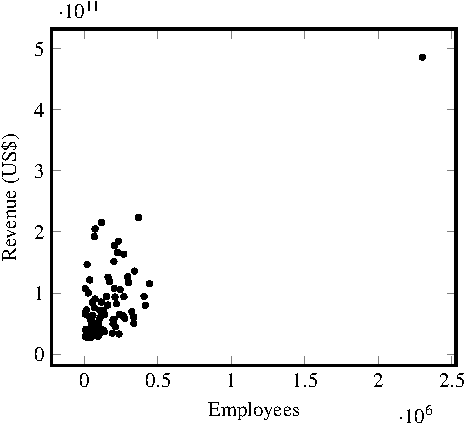
\includegraphics[scale=0.8]{image/12/fortune100-linear.pdf}
  \label{fig:logarithm:Fortune100_linear}
}
%%
%%
\subfigure[]{
  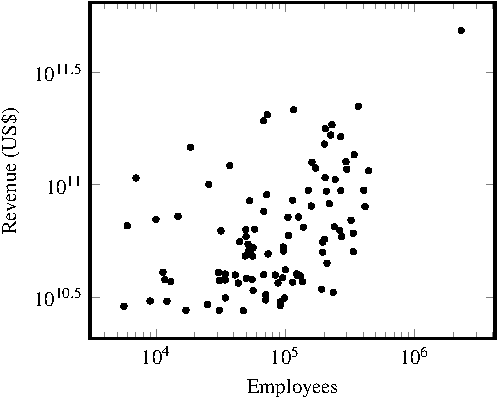
\includegraphics[scale=0.8]{image/12/fortune100-log.pdf}
  \label{fig:logarithm:Fortune100_log}
}
\caption{%%
  The number of employees versus the revenue of the top $100$ US
  companies.  Revenue is in US dollars.  (a)~A scatter plot with
  linear axes.  Each value on the horizontal and vertical axes should
  be multiplied by, respectively, $10^6$ and $10^{11}$.  (b)~A scatter
  plot with log-log axes.
}
\label{fig:logarithm:Fortune100}
\end{figure}

\begin{table}[!htbp]
\centering
\begin{tabular}{ccrrcc} \toprule
Diameter & Volume &&& Diameter & Volume  \\\midrule
$4.4$    & $2.0$  &&& $11.0$   & $25.8$  \\
$4.6$    & $2.2$  &&& $11.1$   & $32.8$  \\
$5.0$    & $3.0$  &&& $11.2$   & $35.4$  \\
$5.1$    & $4.3$  &&& $11.5$   & $26.0$  \\
$5.1$    & $3.0$  &&& $11.7$   & $29.0$  \\
$5.2$    & $2.9$  &&& $12.0$   & $30.2$  \\
$5.2$    & $3.5$  &&& $12.2$   & $28.2$  \\
$5.5$    & $3.4$  &&& $12.2$   & $32.4$  \\
$5.5$    & $5.0$  &&& $12.5$   & $41.3$  \\
$5.6$    & $7.2$  &&& $12.9$   & $45.2$  \\
$5.9$    & $6.4$  &&& $13.0$   & $31.5$  \\
$5.9$    & $5.6$  &&& $13.1$   & $37.8$  \\
$7.5$    & $7.7$  &&& $13.1$   & $31.6$  \\
$7.6$    & $10.3$ &&& $13.4$   & $43.1$  \\
$7.6$    & $8.0$  &&& $13.8$   & $36.5$  \\
$7.8$    & $12.1$ &&& $13.8$   & $43.3$  \\
$8.0$    & $11.1$ &&& $14.3$   & $41.3$  \\
$8.1$    & $16.8$ &&& $14.3$   & $58.9$  \\
$8.4$    & $13.6$ &&& $14.6$   & $65.6$  \\
$8.6$    & $16.6$ &&& $14.8$   & $59.3$  \\
$8.9$    & $20.2$ &&& $14.9$   & $41.4$  \\
$9.1$    & $17.0$ &&& $15.1$   & $61.5$  \\
$9.2$    & $17.7$ &&& $15.2$   & $66.7$  \\
$9.3$    & $19.4$ &&& $15.2$   & $68.2$  \\
$9.3$    & $17.1$ &&& $15.3$   & $73.2$  \\
$9.8$    & $23.9$ &&& $15.4$   & $65.9$  \\
$9.9$    & $22.0$ &&& $15.7$   & $55.5$  \\
$9.9$    & $23.1$ &&& $15.9$   & $73.6$  \\
$9.9$    & $22.6$ &&& $16.0$   & $65.9$  \\
$10.1$   & $22.0$ &&& $16.8$   & $71.4$  \\
$10.2$   & $27.0$ &&& $17.8$   & $80.2$  \\
$10.2$   & $27.0$ &&& $18.3$   & $93.8$  \\
$10.3$   & $27.4$ &&& $18.3$   & $97.9$  \\
$10.4$   & $25.2$ &&& $19.4$   & $107.0$ \\
$10.6$   & $25.5$ &&& $23.4$   & $163.5$ \\\bottomrule
\end{tabular}

\caption{%%
  The diameter versus volume of $70$ shortleaf pine trees.  The
  diameter of a tree is measured in inches and the volume of a tree is
  measured in cubic feet.
}
\label{tab:logarithm:shortleaf}
\end{table}

\begin{figure}[!htbp]
\centering
\subfigure[]{
  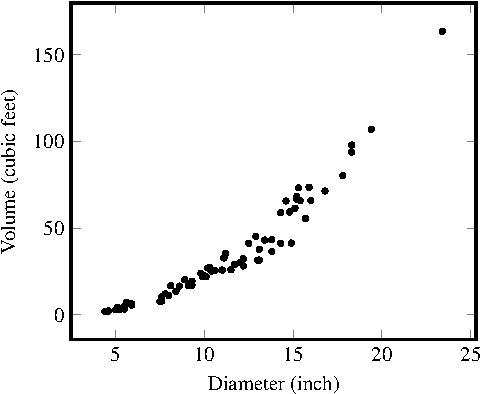
\includegraphics[scale=0.8]{image/12/shortleaf-linear.pdf}
  \label{fig:logarithm:shortleaf_linear}
}
%%
%%
\subfigure[]{
  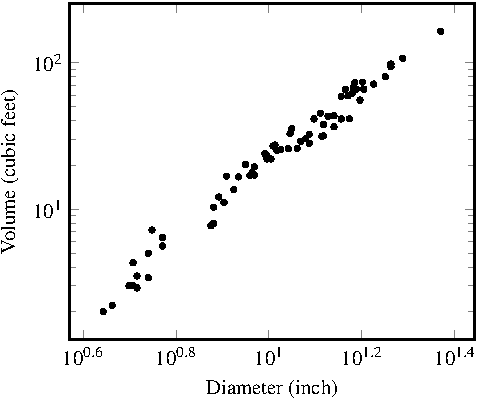
\includegraphics[scale=0.8]{image/12/shortleaf-log.pdf}
  \label{fig:logarithm:shortleaf_log}
}
\caption{%%
  Graphs of the shortleaf pine data in
  \Table{tab:logarithm:shortleaf}.  (a)~A scatter plot with linear
  scaling on both of the horizontal and vertical axes.  (b)~The same
  scatter plot, but with logarithmic scaling on both of the horizontal
  and vertical axes.
}
\label{fig:logarithm:shortleaf_linear_log}
\end{figure}

Let's consider a data set that can be used to perform regression.
\Table{tab:logarithm:shortleaf} lists the diameter~(inch) versus
volume~(cubic feet) of $70$ shortleaf pine trees.\footnote{
  The data set was published in the book:
  D.~Bruce and F.~X.~Schumacher.  \emph{Forest mensuration}.
  McGraw-Hill Book Company, 1935.
  The data set was downloaded from
  \url{http://web.archive.org/web/20180518051945/https://newonlinecourses.science.psu.edu/stat501/sites/onlinecourses.science.psu.edu.stat501/files/data/shortleaf/index.txt},
  accessed 2018-05-18.
}
The data set is graphed in \Figure{fig:logarithm:shortleaf_linear}
with linear scaling for both of the horizontal and vertical axes.  The
figure seems to show that the data follow an exponential function.
\Figure{fig:logarithm:shortleaf_log} shows the same graph, but using
logarithmic scaling for both axes.  The figure shows that the points
seem to follow a straight line.  So how would you use a linear
function to model the dots in \Figure{fig:logarithm:shortleaf_log}?

Let's start by defining some variables.  Denote by $Q(x)$ the
volume~(in cubic feet) of a shortleaf pine tree that has a diameter of
$x$ inches.  Suppose that the function $Q(x)$ models the points in
\Figure{fig:logarithm:shortleaf_linear}.  When you go from the linear
scaling in \Figure{fig:logarithm:shortleaf_linear} to the log-log
scaling in \Figure{fig:logarithm:shortleaf_log}, assume that you take
the natural logarithm of each value in the ``Diameter'' and ``Volume''
columns of \Table{tab:logarithm:shortleaf}.  The function $Q(x)$ now
becomes $\ln Q(x)$ and the variable $x$ now becomes $\ln x$.  As the
points in \Figure{fig:logarithm:shortleaf_log} seem to follow a linear
function, then you can model the points as
%%
\begin{equation}
\label{eqn:logarithm:log_log_regression}
\ln Q(x)
=
a \cdot \ln x + b
\end{equation}
%%
where the parameters $a$ and $b$ are to be estimated from the data in
\Table{tab:logarithm:shortleaf}.  Just as you have done
in \Section{subsec:logarithm:logarithmic_scaling_on_horizontal_axis},
the values of $a$ and $b$ are treated as the parameters $\alphahat$
and $\betahat$, respectively, in the linear regression function.  Now
suppose that you have estimated the parameters $a$ and $b$.  You still
need to solve \Equation{eqn:logarithm:log_log_regression} for $Q(x)$.
By treating both sides of \Equation{eqn:logarithm:log_log_regression}
as exponents of $e$, you can write the equation as
$e^{\ln Q(x)} = e^{a \cdot \ln x + b}$, which by
\Subtheorem{thm:logarithm:cancellation_property}{subthm:logarithm:cancellation_property_exponential_log}
simplifies to $Q(x) = e^{a \cdot \ln x + b}$.  The latter equation can
also be written as $Q(x) = e^{a \cdot \ln x} \cdot e^b$ and use the
power rule of
\Subtheorem{thm:logarithm:properties}{thm:logarithm:properties_multiplication}
to write $Q(x) = e^{\ln(x^a)} \cdot e^b$, which by
\Subtheorem{thm:logarithm:cancellation_property}{subthm:logarithm:cancellation_property_exponential_log}
again simplifies to $Q(x) = x^a \cdot e^b$.  Therefore
\Equation{eqn:logarithm:log_log_regression} can be solved for $Q(x)$
to produce
%%
\begin{equation}
\label{eqn:logarithm:power_regression}
Q(x)
=
e^b x^a
\end{equation}
%%
where the parameters $a$ and $b$ must be estimated from the data set.
Note that $Q(x)$ as defined in~\eqref{eqn:logarithm:power_regression}
is not a logarithmic function, but a power function.  When you use
linear regression to estimate the parameters $a$ and $b$ of $Q(x)$,
you are performing what is called \emph{power regression}.

\begin{example}
\label{eg:logarithm:shortleaf_pine_trees}
\textbf{Shortleaf pine trees.}
Consider the data in \Table{tab:logarithm:shortleaf} on the diameter
versus volume of $70$ shortleaf pine trees.
%%
\begin{packedenum}
\item\label{subeg:logarithm:shortleaf_power_regression}
  Suppose that the data in the table follow the function
  $V(x) = e^b x^a$, where $V(x)$ denotes the volume in cubic feet of a
  shortleaf pine tree that has a diameter of $x$ inches.  Use power
  regression to estimate the parameters $a$ and $b$.  Graph the model
  $V(x)$ together with the scatter plot of
  \Figure{fig:logarithm:shortleaf_linear}.

\item\label{subeg:logarithm:shortleaf_Pearson_r_RMS_error}
  Calculate the coefficient of determination $R^2$ and root mean
  square~(RMS) error of the function $V(x)$
  from \Part{subeg:logarithm:shortleaf_power_regression}.  Provide an
  interpretation of the values of $R^2$ and the RMS error.
\end{packedenum}
\end{example}

\begin{solution}
\solutionpart{subeg:logarithm:shortleaf_power_regression}
First, you must take the natural logarithm of each value in the
``Diameter'' columns of \Table{tab:logarithm:shortleaf} and store the
results in a separate column; let's call this column $w$.  Do the same
calculation for the ``Volume'' columns and store the results in
another separate column; call this column $v$.  Second, perform linear
regression on the numbers in the $w$ and $v$ columns.  The means of
the $w$ and $v$ columns are $\wbar \approx 2.3407$ and
$\vbar \approx 3.1307$, respectively.  If $w_i$ is the value in row
$i$ of the $w$ column, then define $d(w_i) = w_i - \wbar$.  Similarly,
define $d(v_i) = v_i - \vbar$.  You now have the sums
\[
\sum_{i=1}^n (w_i - \wbar) (v_i - \vbar)
\approx
28.3630
%%
\qquad
\text{and}
\qquad
%%
\sum_{i=1}^n (w_i - \wbar)^2
\approx
11.0602
\]
where $n = 70$ is the number of data points in
\Table{tab:logarithm:shortleaf}.  Use the above sums to obtain the
parameter estimates
%%
\begin{align*}
\alphahat
&=
\frac{
  \sum_{i=1}^n (w_i - \wbar) (v_i - \vbar)
}{
  \sum_{i=1}^n (w_i - \wbar)^2
}
\approx
2.5644 \\[4pt]
%%
%%
\betahat
&=
\vbar - \alphahat \wbar
\approx
-2.8718
\end{align*}
%%
which yield the estimates $e^b \approx 0.0566$ and
$a \approx 2.5644$.  If $V(x)$ represents the volume~(cubic feet) of a
shortleaf pine tree that has a diameter of $x$ inches, then the volume
can be written as
%%
\begin{equation}
\label{eqn:logarithm:shortleaf_volume}
V(x)
=
0.0566 x^{2.5644}.
\end{equation}
%%
\Figure{fig:logarithm:shortleaf_volume} shows a graph of the model
together with the data from \Table{tab:logarithm:shortleaf}.

\begin{figure}[!htbp]
\centering
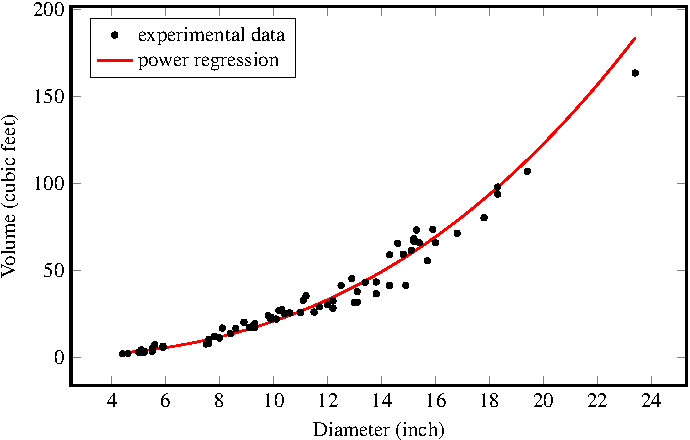
\includegraphics[scale=1.1]{image/12/shortleaf.pdf}
\caption{%%
  The diameter of a shortleaf pine tree versus its volume.  The black
  dots show the data from \Table{tab:logarithm:shortleaf}.  The red
  curve is a graph of \Equation{eqn:logarithm:shortleaf_volume}.
}
\label{fig:logarithm:shortleaf_volume}
\end{figure}

\solutionpart{subeg:logarithm:shortleaf_Pearson_r_RMS_error}
The model~\eqref{eqn:logarithm:shortleaf_volume} has a coefficient of
determination of $R^2 \approx 0.9736$ and a root mean
square~(RMS) error of approximately $5.7532$.  The high value of $R^2$
and the low value of the RMS error both suggest that
\Equation{eqn:logarithm:shortleaf_volume} fits the data very well.
\end{solution}

\begin{exercise}
\textbf{Shortleaf pine trees.}
In \Example{eg:logarithm:shortleaf_pine_trees}, the plot of
\Figure{fig:logarithm:shortleaf_volume} seems to suggest that the data
on shortleaf pine trees follow an exponential function.  Assume that
the data approximately follow the exponential function
$f(x) = a \cdot e^{rx}$, where $f(x)$ represents the volume~(cubic
feet) of a shortleaf pine tree that has a diameter of $x$ inches.
%%
\begin{packedenum}
\item\label{subex:logarithm:shortleaf_exponential_regression}
  Use exponential regression to estimate the parameters $a$ and $r$.
  Plot the function $f(x)$ together with the graph in
  \Figure{fig:logarithm:shortleaf_volume}.

\item\label{subex:logarithm:shortleaf_exponential_R^2_RMS_error}
  Calculate the coefficient of determination and the root mean square
  error of the function $f(x)$.  Compare these values with the
  corresponding values in \Example{eg:logarithm:shortleaf_pine_trees}.
  Explain which one of the functions $V(x)$ and $f(x)$ is better at
  fitting the experimental data.
\end{packedenum}
\end{exercise}

\ifbool{showSolution}{
\begin{solution}
\solutionpart{subex:logarithm:shortleaf_exponential_regression}
Let $x$ denote the ``Diameter'' columns of
\Table{tab:logarithm:shortleaf}.  Take the natural logarithm of each
value in the ``Volume'' columns of the table and store the results in
a separate column; call this column $y$.  Since you assume that the
data in the table follow an exponential function, the $y$ column is a
linearisation of the data in the ``Volume'' columns and so
$\ln f(x) = y$.  The $x$ and $y$ columns are related by the linear
function $\ln f(x) = rx + \ln a$, where the parameters $r$ and
$\ln a$ can be estimated by the parameters $\alphahat$ and $\betahat$
of the linear regression of the $x$ and $y$ columns.  The means of the
$x$ and $y$ columns are $\xbar \approx 11.1843$ and
$\ybar \approx 3.1307$, respectively.  You have the sums
\[
\sum_{i=1}^n (x_i - \xbar) (y_i - \ybar)
\approx
282.2806
%%
\qquad
\text{and}
\qquad
%%
\sum_{i=1}^n (x_i - \xbar)^2
\approx
1178.4727
\]
which can be used to produce the parameter estimates
%%
\begin{align*}
\alphahat
&=
\frac{
  \sum_{i=1}^n (x_i - \xbar) (y_i - \ybar)
}{
  \sum_{i=1}^n (x_i - \xbar)^2
}
\approx
0.2395 \\[4pt]
%%
%%
\betahat
&=
\ybar - \alphahat \xbar
\approx
0.4517
\end{align*}
%%
where $n = 70$ is the number of data points in
\Table{tab:logarithm:shortleaf}.  Then $f(x)$ can be written as
%%
\begin{equation}
\label{eqn:logarithm:shortleaf_compare_exponential_power}
f(x)
=
1.571 e^{0.2395 x}.
\end{equation}
%%
\Figure{fig:logarithm:shortleaf_compare_exponential_power} shows a
graph of \Equation{eqn:logarithm:shortleaf_compare_exponential_power}
together with the plot in \Figure{fig:logarithm:shortleaf_volume}.

\begin{figure}[!htbp]
\centering
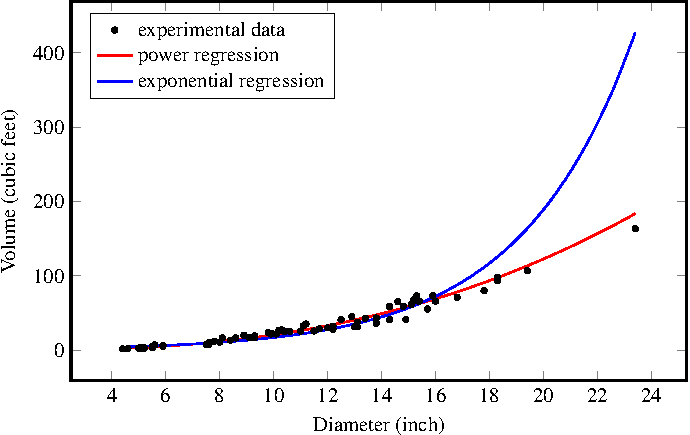
\includegraphics[scale=1.1]{image/12/shortleaf-compare.pdf}
\caption{%%
  Comparison of two prediction functions for the shortleaf pine data
  in \Table{tab:logarithm:shortleaf}.  The red and blue curves are
  graphs of
  \Equations{eqn:logarithm:shortleaf_volume}{eqn:logarithm:shortleaf_compare_exponential_power},
  respectively.
}
\label{fig:logarithm:shortleaf_compare_exponential_power}
\end{figure}

\solutionpart{subex:logarithm:shortleaf_exponential_R^2_RMS_error}
The exponential model $f(x)$ as defined in
\Equation{eqn:logarithm:shortleaf_compare_exponential_power} has a
coefficient of determination of $R^2 \approx 0.9051$ and a root mean
square~(RMS) error of approximately $33.3568$.  The value of $R^2$ of
$f(x)$ is smaller than the corresponding value for the power model
$V(x)$ as defined in \Equation{eqn:logarithm:shortleaf_volume}.
Furthermore, the RMS error of $f(x)$ is higher than the RMS error of
$V(x)$.  Based on these results, you may conclude that $V(x)$ is
better than $f(x)$ at modelling the shortleaf pine data.
\end{solution}
}{}

\begin{table}[!htbp]
\centering
\begin{tabular}{lrr} \toprule
\multicolumn{1}{c}{Site} & \multicolumn{1}{c}{Average weight} & \multicolumn{1}{c}{Density} \\\midrule
China, Shucheng, Anhui          & $3122.33333333333$  & $3.0000$   \\
China, Shucheng, Anhui          & $4166.93333333333$  & $3.7500$   \\
China, Shucheng, Anhui          & $2267.11111111111$  & $4.5000$   \\
China, Shucheng, Anhui          & $2306.28571428571$  & $5.2500$   \\
China, Junyun Mountain, Sichuan & $2228.69763465375$  & $7.0180$   \\
China, Dagang Mountain, Jiangxi & $21872.30989956960$ & $0.2788$   \\
China, Dagang Mountain, Jiangxi & $22125.64102564100$ & $0.3900$   \\
China, Dagang Mountain, Jiangxi & $21903.19031903190$ & $0.4545$   \\
China, Baishui, Gansu           & $2500.46153846153$  & $6.5000$   \\
Japan, Nagano                   & $4.01028277633$     & $389.0000$ \\
Japan, Nagano                   & $12.30769230768$    & $260.0000$ \\
Japan, Nagano                   & $12.91666666665$    & $216.0000$ \\
Japan, Nagano                   & $84.36363636361$    & $27.5000$  \\\bottomrule
\end{tabular}

\caption{%%
  The average weight versus density of $13$ populations of bamboo.
  Each average weight is measured in grams and is the mean of the
  weight of the shoots of a bamboo population.  The density of a
  population of bamboo is defined as the number of bamboo shoots per
  square metre.
}
\label{tab:logarithm:bamboo}
\end{table}

\begin{exercise}
\textbf{Bamboo.}
\Table{tab:logarithm:bamboo} shows the average weight versus density
of $13$ populations of bamboo in China and Japan.\footnote{
  The data set was published in the paper:
  \url{https://doi.org/10.1073/pnas.1205663109}
}
%%
\begin{packedenum}
\item\label{subex:logarithm:bamboo_linear_log}
  Produce two graphs of the average weight versus density.  One graph
  uses linear scaling for both of the horizontal and vertical axes.
  The other graph uses logarithmic scaling for both axes.  What do you
  notice in both graphs?

\item\label{subex:logarithm:bamboo_power_regression}
  Denote by $D(x)$ the density of a bamboo population that has a mean
  weight of $x$ grams.  Suppose that the data in
  \Table{tab:logarithm:bamboo} follow a power function of the form
  $D(x) = e^b x^a$.  Use power regression to estimate the parameters
  $a$ and $b$.  Graph the function $D(x)$ together with the data from
  the data.  Use logarithmic and linear scalings for the horizontal
  and vertical axes, respectively.  Calculate the coefficient of
  determination and the root mean square error of $D(x)$.

\item\label{subex:logarithm:bamboo_explain}
  Note that in \Table{tab:logarithm:bamboo} as the mean weight of a
  bamboo population increases, the density of the population
  decreases.  Explain why this happened for the $13$ bamboo
  populations.
\end{packedenum}
\end{exercise}

\ifbool{showSolution}{
\begin{solution}
\solutionpart{subex:logarithm:bamboo_linear_log}
\Figure{subfig:logarithm:bamboo_linear} shows a scatter plot of the
data in \Table{tab:logarithm:bamboo} using linear scaling for both of
the horizontal and vertical axes.  The black dots seem to follow a
steep curve that looks like the graph of an exponential decay
function.  \Figure{subfig:logarithm:bamboo_log} shows a scatter plot
of the same data set, but using logarithmic scaling for both axes.
The log-log plot shows that the black dots seem to follow a straight
line.

\begin{figure}[!htbp]
\centering
\subfigure[]{
  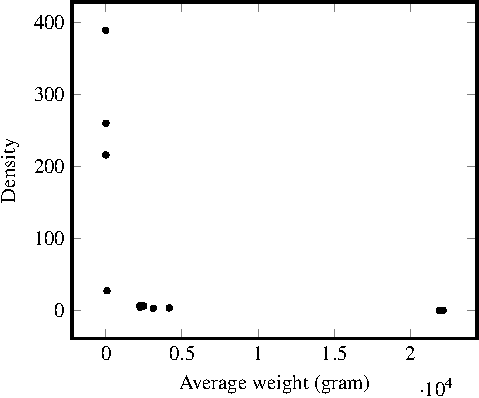
\includegraphics[scale=0.8]{image/12/bamboo-linear.pdf}
  \label{subfig:logarithm:bamboo_linear}
}
%%
%%
\subfigure[]{
  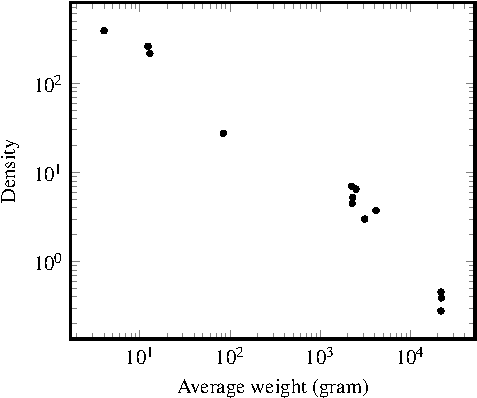
\includegraphics[scale=0.8]{image/12/bamboo-log.pdf}
  \label{subfig:logarithm:bamboo_log}
}
\caption{%%
  The average weight versus density of $13$ populations of bamboo.
  The average weight is measured in grams.  For each bamboo
  population, the density is defined as the number of bamboo shoots
  per squared metre.  (a)~A scatter plot of the data in
  \Table{tab:logarithm:bamboo}, where both of the horizontal and
  vertical axes use linear scaling.  (b)~A scatter plot of the same
  data set, but both axes use logarithmic scaling.
}
\label{fig:logarithm:bamboo_linear_log}
\end{figure}

\solutionpart{subex:logarithm:bamboo_power_regression}
First, you linearise the data.  Take the natural logarithm of each
value in the ``Average weight'' column and store the results in a
separate column; call this column $v$.  Similarly, take the natural
logarithm of each value in the ``Density'' column and store the
results in another separate column called $w$.  Next, you perform
linear regression on the $v$ and $w$ columns.  The means of the $v$
and $w$ columns are $\vbar \approx 6.7899$ and
$\wbar \approx 2.0469$, respectively.  If $v_i$ is the value in row
$i$ of the $v$ column, then define $d(v_i) = v_i - \vbar$.  Similarly,
define $d(w_i) = w_i - \wbar$.  You have the sums
\[
\sum_{i=1}^n (v_i - \vbar) (w_i - \wbar)
\approx
-86.0626
%%
\qquad
\text{and}
\qquad
%%
\sum_{i=1}^n (v_i - \vbar)^2
\approx
109.4650
\]
which can be used to produce the estimates
%%
\begin{align*}
\alphahat
&=
\frac{
  \sum_{i=1}^n (v_i - \vbar) (w_i - \wbar)
}{
  \sum_{i=1}^n (v_i - \vbar)^2
}
\approx
-0.7862 \\[4pt]
%%
%%
\betahat
&=
\wbar - \alphahat \vbar
\approx
7.3852
\end{align*}
%%
where $n = 13$ is the number of data points in
\Table{tab:logarithm:bamboo}.  You treat $\alphahat$ and $\betahat$ as
estimates of the parameters $a$ and $b$, respectively, so that
$e^{\betahat} \approx 1611.9147$.  Thus the function $D(x)$ can be
written as
%%
\begin{equation}
\label{eqn:logarithm:bamboo_power_regression}
D(x)
=
1611.9147 x^{-0.7862}.
\end{equation}
%%
\Figure{fig:logarithm:bamboo} compares the prediction of
\Equation{eqn:logarithm:bamboo_power_regression} against the
experimental data.  Note that the horizontal axis uses logarithmic
scaling, but the vertical axis uses linear scaling.  The function
$D(x)$ has a coefficient of determination of $R^2 \approx 0.9624$ and
a root mean square error of approximately $43.7429$.

\begin{figure}[!htbp]
\centering
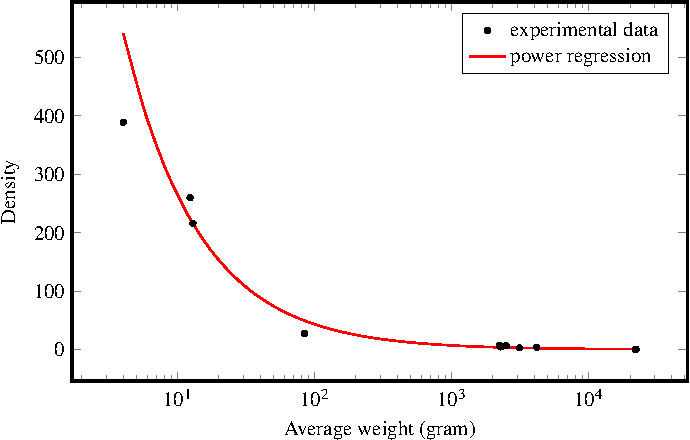
\includegraphics[scale=1.1]{image/12/bamboo.pdf}
\caption{%%
  The mean weight versus density of $13$ populations of bamboo.  The
  black dots show the data from \Table{tab:logarithm:bamboo}.  The red
  curve is a graph of
  \Equation{eqn:logarithm:bamboo_power_regression}.
}
\label{fig:logarithm:bamboo}
\end{figure}

\solutionpart{subex:logarithm:bamboo_explain}
\Figure{fig:logarithm:bamboo} shows that as the mean weight of a
bamboo population increases the density of the population decreases.
An increase in mean weight corresponds to, on average, an increase in
the weight of individual bamboo shoots in a population.  As the bamboo
shoots compete for resources to grow, the larger shoots require more
resources than the smaller shoots, which translates to less resources
for the smaller shoots.  In a bamboo population where the majority of
shoots have low mean weight, you tend to have more shoots growing to
maturity.  However, as the majority of bamboo shoots have higher and
higher mean weight, you tend to have less and less shoots growing to
maturity.  The competition for resources exerts pressure on and limits
the population density of bamboos.
\end{solution}
}{}

\begin{table}[!htbp]
\centering
\begin{tabular}{lcc} \toprule
        & Distance to \\
Planet  & Sun~(Gm) & Orbital period \\\midrule
Mercury & $57.9$   & $88.0$     \\
Venus   & $108.2$  & $224.7$    \\
Earth   & $149.6$  & $365.2$    \\
Mars    & $227.9$  & $687.0$    \\
Jupiter & $778.6$  & $4331.0$   \\
Saturn  & $1433.5$ & $10,747.0$ \\
Uranus  & $2872.5$ & $30,589.0$ \\
Neptune & $4495.4$ & $59,800.0$ \\
Pluto   & $5906.4$ & $90,560.0$ \\\bottomrule
\end{tabular}

\caption{%%
  The distance to the Sun versus the orbital period of a planet.
  Distance is measured in gigametres, where one gigametre~(or $1$~Gm)
  is equivalent to $10^6$ kilometres.  The orbital period of a planet
  is the number of Earth days required for the planet to complete one
  orbit around the Sun.
}
\label{tab:logarithm:orbital_period}
\end{table}

\begin{exercise}
\textbf{Orbital period.}
\Table{tab:logarithm:orbital_period} lists for each planet the
distance from the planet to the Sun and the planet's orbital period.
The data are provided by NASA.\footnote{
  See the following website:
  \url{http://web.archive.org/web/20180427010804/https://nssdc.gsfc.nasa.gov/planetary/factsheet/},
  accessed 2018-04-27.
}
%%
\begin{packedenum}
\item\label{subex:logarithm:planets_scatter_plots}
  Produce two scatter plots of the data in
  \Table{tab:logarithm:orbital_period}.  One graph should use linear
  scaling for both of the horizontal and vertical axes.  The other
  graph should use logarithmic scaling for both axes.  Explain what
  you notice about the graphs.

\item\label{subex:logarithm:planets_power_regression}
  Let $P(x)$ be the orbital period of a planet that is $x$ gigametres
  away from the Sun.  Use power regression to derive an expression for
  $P(x)$.  Graph your formula together with a scatter plot of the data
  in \Table{tab:logarithm:orbital_period}.  Calculate the coefficient
  of determination of your formula.

\item\label{subex:logarithm:planets_Kepler}
  If $K(x)$ represents the orbital period of a planet that is at a
  distance of $x$ gigametres from the Sun, then Kepler showed that
  $K(x)$ can be written as
  %%
  \begin{equation}
  \label{eqn:logarithm:planets_Kepler_formula}
  K(x)
  =
  0.1996 x^{1.5}.
  \end{equation}
  %%
  Use the root mean square error to help you decide which one of
  $P(x)$ and $K(x)$ is better than the other at modelling the data in
  \Table{tab:logarithm:orbital_period}.
\end{packedenum}
\end{exercise}

\ifbool{showSolution}{
\begin{solution}
\solutionpart{subex:logarithm:planets_scatter_plots}
\Figure{subfig:logarithm:planets_linear} shows a scatter plot of the
data in \Table{tab:logarithm:orbital_period} and using linear scaling
for both of the horizontal and vertical axes.  The graph shows that
the dots seem to follow an exponential function.  The same scatter
plot is shown in \Figure{subfig:logarithm:planets_log}, but using
logarithmic scaling for the axes.  The log-log plot shows that the
dots seem to follow a straight line, which suggests that you can use
power regression to model the data.

\begin{figure}[!htbp]
\centering
\subfigure[]{
  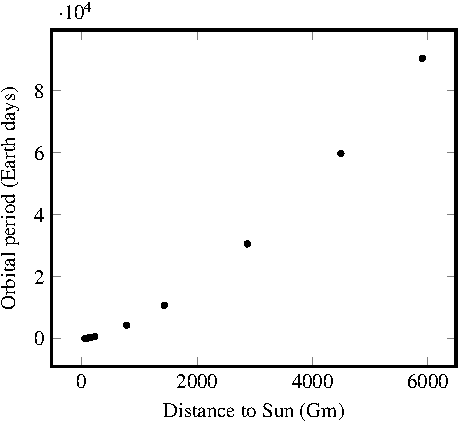
\includegraphics[scale=0.8]{image/12/planets-linear.pdf}
  \label{subfig:logarithm:planets_linear}
}
%%
%%
\subfigure[]{
  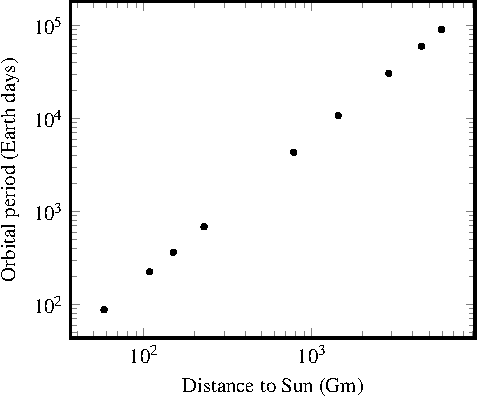
\includegraphics[scale=0.8]{image/12/planets-log.pdf}
  \label{subfig:logarithm:planets_log}
}
\caption{%%
  The distance of a planet to the Sun versus the planet's orbital
  period.  Distance is measured in gigametres and orbital period is
  measured in Earth days.  (a)~A scatter plot that uses linear scaling
  for both of the horizontal and vertical axes.  Note that each value
  on the vertical axis must be multiplied by $10^4$.  (b)~The same
  scatter plot, but using logarithmic scaling for both axes.
}
\label{fig:logarithm:planets}
\end{figure}

\begin{figure}[!htbp]
\centering
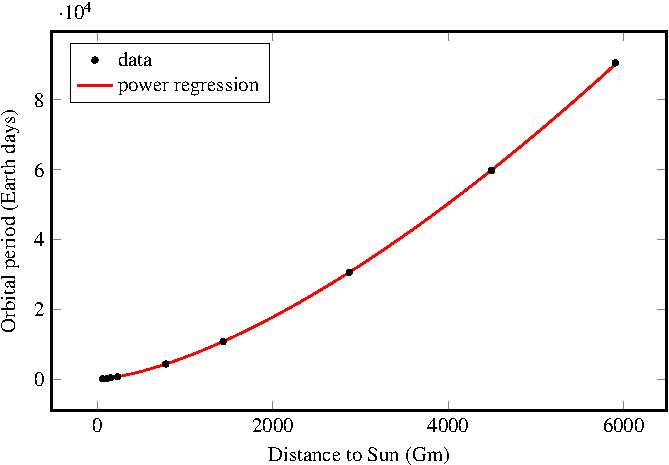
\includegraphics[scale=1.1]{image/12/planets.pdf}
\caption{%%
  The distance of a planet to the Sun versus the planet's orbital
  period.  The black dots show a scatter plot of the data in
  \Table{tab:logarithm:orbital_period}.  The red curve shows a graph
  of \Equation{eqn:logarithm:planets_power_regression}.  Each value on
  the vertical axis must be multiplied by $10^4$.
}
\label{fig:logarithm:planets_regression}
\end{figure}

\solutionpart{subex:logarithm:planets_power_regression}
Let $P(x)$ be the orbital period of a planet that is at a distance of
$x$ gigametres from the Sun.  Power regression on the data in
\Table{tab:logarithm:orbital_period} shows that $P(x)$ can be written
as
%%
\begin{equation}
\label{eqn:logarithm:planets_power_regression}
P(x)
=
0.2007 x^{1.4988}.
\end{equation}
%%
The function is compared in \Figure{fig:logarithm:planets_regression}
with the data in \Table{tab:logarithm:orbital_period}.
Equation~\eqref{eqn:logarithm:planets_power_regression} has a
coefficient of determination of $R^2 \approx 0.9999$.

\solutionpart{subex:logarithm:planets_Kepler}
The model~\eqref{eqn:logarithm:planets_power_regression} has a root
mean square~(RMS) error of approximately $138.0027$.  This is slightly
higher than the RMS error of
\Equation{eqn:logarithm:planets_Kepler_formula}, which has an RMS
error of approximately $132.9641$.  Conclude that Kepler's
\Equation{eqn:logarithm:planets_Kepler_formula} is better than
\Equation{eqn:logarithm:planets_power_regression} at modelling the
data in \Table{tab:logarithm:orbital_period}.
\end{solution}
}{}


\newpage
%%%%%%%%%%%%%%%%%%%%%%%%%%%%%%%%%%%%%%%%%%%%%%%%%%%%%%%%%%%%%%%%%%%%%%%%%%%

\section*{Problem}

\begin{problem}
\item Read the following article by Kathleen M. Clark and Clemency
  Montelle:
  \emph{Logarithms: The Early History of a Familiar Function}.\footnote{
    The article is available at the website
    \url{http://web.archive.org/web/20180509072424/https://www.maa.org/press/periodicals/convergence/logarithms-the-early-history-of-a-familiar-function},
    accessed 2018-05-09.
  }

\item Pressure and density above sea level.
\ifbool{showSolution}{
\begin{solution}

\end{solution}
}{}

\item Why can't the base be $b = 1$?
\ifbool{showSolution}{
\begin{solution}

\end{solution}
}{}

\item Prove the half-life formula for radioactive decay.  Derive the
  rule of $69$ for the half-life of an exponential decay model.
\ifbool{showSolution}{
\begin{solution}

\end{solution}
}{}

\item Prove the doubling-time formula for an exponential growth
  model.
\ifbool{showSolution}{
\begin{solution}

\end{solution}
}{}

\item\emph{Newton's law of cooling.}
  A forensic team arrived at the scene of a crime and found the dead
  body of an adult human.  The team measured the temperature of the
  body to be $\degreec{26}$ and noted that the time was 3:25~pm.  One
  hour later, the team again measured the temperature of the body and
  found that the body had cooled down to $\degreec{24}$.  The body was
  located in a room that was known to have a constant temperature of
  $\degreec{15}$.
  %%
  \begin{packedenum}
  \item\label{subprob:logarithm:Newton_forensic_formula}
    Let $T(t)$ be the temperature in degrees Celsius of the body at
    $t$ hours since 3:25~pm.  Use Newton's law of cooling and the
    above information to write a formula for $T(t)$.  The rate of
    cooling is the constant $k$.  Solve your formula for $k$ to
    determine the value of the rate of cooling.

  \item\label{subprob:logarithm:Newton_forensic_time_of_death}
    The normal body temperature of a live adult human is approximately
    $\degreec{37}$.\footnote{
      Further details are available in the paper
      \url{https://doi.org/10.1046/j.1471-6712.2002.00069.x}.
    }
    Estimate the time of death of the victim.
  \end{packedenum}
\ifbool{showSolution}{
\begin{solution}
\solutionpart{subprob:logarithm:Newton_forensic_formula}
Let $t$ be the number of hours since 3:25~pm so that the time of
$t = 0$ corresponds to 3:25~pm itself.  The initial temperature of the
body was $T_0 = 26$ degrees Celsius.  At time $t = 1$ hour after
3:25~pm~(i.e.~at 4:25~pm), the temperature of the body was
$T(1) = 24$ degrees Celsius.  The constant temperature of the
surrounding was $T_s = 15$ degrees Celsius.  Substitute these values
into \Equation{eqn:logarithm:Newton_law_cooling} to obtain
%%
\begin{align*}
T(1)
&=
15 + (26 - 15) e^{-k \times 1} \\[4pt]
&=
15 + 11e^{-k} \\[4pt]
&=
24.
\end{align*}
%%
The latter equation can also be written as
$\frac{24 - 15}{11} = e^{-k}$, which simplifies to
$\frac{9}{11} = e^{-k}$.  Take the natural logarithm of both sides to
get $\ln \frac{9}{11} = -k$ and solving for $k$ shows that
$k = -\ln \frac{9}{11}$.

\solutionpart{subprob:logarithm:Newton_forensic_time_of_death}
The temperature $T(t)$ of the body at $t$ hours since 3:25~pm is
\[
T(t)
=
15 + 11 e^{-kt}
\]
where $k = -\ln \frac{9}{11}$ is the rate of cooling.  You want to
determine the value of $t$ such that $T(t) = 37$ degrees Celsius.
That is, you want to solve the equation $37 = 15 + 11 e^{-kt}$ for
$t$.  The equation can be written as
$\frac{37 - 15}{11} = e^{-kt}$, which simplifies to $2 = e^{-kt}$.
Take the natural logarithm of both sides to get $\ln 2 = -kt$ and
solving for $t$ shows that
$t = -\frac{1}{k} \ln 2 \approx -3.454152$.  That is, the victim died
at approximately $3.454152$ hours before 3:25~pm.  Three hours before
3:25~pm would be 12:25~noon.  Multiply the fractional part $0.454152$
by $60$ minutes to get $0.454152 \times 60 = 27.24912 \approx 27$
minutes.  The time of $27$ minutes before 12:25~noon would be
11:58~am.  Thus the victim died at approximately 11:58~am on the day
the body was discovered.
\end{solution}
}{}

\item Analysis of linear search and binary search.
\ifbool{showSolution}{
\begin{solution}

\end{solution}
}{}

\item\emph{Preston curve.}
  In economics, the \emph{gross domestic product}~(GDP) per capita is
  a measure of the average income of a country.  The higher is the GDP
  per capita of a country, the higher is the standard of living of the
  country's population.  One way to measure the health of the
  population of a country is to calculate the
  \emph{life expectancy at birth} for the country.  The life
  expectancy at birth can be interpreted as the average number of
  years that a newborn baby is expected to live.  The higher is the
  life expectancy at birth for the population of a country, the
  healthier is the population.  In this problem, you will investigate
  the trends in the GDP per capita of Australia and the life
  expectancy at birth of the population of Australia.
  %%
  \begin{packedenum}
  \item\label{subprob:logarithm:Australia_data}
    Go to the website of the World Bank, in particular the page for
    the data that the World Bank collects.\footnote{
      \url{https://data.worldbank.org}
    }
    Search for and download historical statistics for Australia on the
    following: (1)~gross domestic product; (2)~total population
    numbers; and (3)~life expectancy at birth.  For each of the latter
    three categories, you should download statistics for the years
    from~1960 up to and including~2016.  Note that you should download
    the GDP with ``constant 2010 US\$''.  This means that the GDP has
    been adjusted for price inflation in terms of the value of the US
    dollar in the year 2010.

  \item\label{subprob:logarithm:Australia_life_expectancy}
    Produce a graph of the year versus the life expectancy at birth
    between the years $1960$ and $2016$, inclusive.  Recall that for a
    linear function $f(x) = ax + b$, the rate of change $a$~(or
    gradient) is the average change in the vertical direction.  Let
    $L(x)$ be the life expectancy at birth of Australia for the year
    $x$.  A graph of $L(x)$ for the years between $1960$ and $2016$,
    inclusive, does not show a straight line.  However, you can
    approximate the rate of change of $L(x)$ by using the gradient of
    a linear function.  Suppose you want to calculate the rate of
    change of the life expectancy at birth of Australia for the year
    $x$.  You consider one year before $x$ and one year after $x$.
    Let $L(x - 1)$ and $L(x + 1)$ be the life expectancy at birth for
    the years $x - 1$ and $x + 1$, respectively.  You suppose that the
    points $\tuple{x-1}{L(x-1)}$ and $\tuple{x+1}{L(x+1)}$ lie on a
    straight line and calculate the gradient of the straight line as
    %%
    \begin{equation}
    \label{eqn:logarithm:Australia_rate_of_change_life_expectancy}
    \begin{aligned}
    \Delta L(x)
    &=
    \frac{
      L(x + 1) - L(x - 1)
    }{
      (x + 1) - (x - 1)
    } \\[4pt]
    &=
    \frac{
      L(x + 1) - L(x - 1)
    }{
      2
    }.
    \end{aligned}
    \end{equation}
    %%
    The gradient $\Delta L(x)$ can be used as an approximation of the
    rate of change in the life expectancy at birth for the year $x$.
    Use
    \Equation{eqn:logarithm:Australia_rate_of_change_life_expectancy}
    to approximate the rate of change in the life expectancy at birth
    of Australia for the years $x = \seq{1961}{1962}{2015}$.  Note
    that you can neither calculate $\Delta L(1960)$ nor
    $\Delta L(2016)$ because you do not have the life expectancies at
    birth for the years $1959$ and $2017$, respectively.  Graph the
    year versus the rate of change of the life expectancy at birth.
    Provide an interpretation of
    \Expression{eqn:logarithm:Australia_rate_of_change_life_expectancy},
    in particular when $\Delta L(x) < 0$, $\Delta L(x) = 0$, and
    $\Delta L(x) > 0$.

  \item\label{subprob:logarithm:Australia_life_expectancy_formula}
    Use the graph
    from \Part{subprob:logarithm:Australia_life_expectancy} to help
    you determine a formula for the life expectancy at birth of
    Australia during the years from $1960$ to $2016$, inclusive.
    Determine the coefficient of determination and the root mean
    square error of your formula.

  \item\label{subprob:logarithm:Australia_GDP_per_capita}
    For a given year $x$, the GDP per capita of a country is defined
    as the GDP for year $x$ divided by the total population for the
    same year.  Calculate the GDP per capita of Australia for each
    year from~1960 up to and including 2016.  Produce a graph of the
    year versus the GDP per capita.  You can use the same technique as
    in
    \Expression{eqn:logarithm:Australia_rate_of_change_life_expectancy}
    to approximate the rates of change in the GDP per capita of
    Australia.  Let $G(x)$ be the GDP per capita of Australia for the
    year $x$.  To approximate how much $G(x)$ has changed since the
    previous year, you consider the GDP per capita of one year before
    $x$ and one year after $x$.  You treat the points
    $\tuple{x-1}{G(x-1)}$ and $\tuple{x+1}{G(x+1)}$ as points on a
    straight line and calculate the gradient of the straight line as
    %%
    \begin{equation}
    \label{eqn:logarithm:Australia_GDP_per_capita_rates}
    \begin{aligned}
    \Delta G(x)
    &=
    \frac{
      G(x + 1) - G(x - 1)
    }{
      (x + 1) - (x - 1)
    } \\[4pt]
    &=
    \frac{
      G(x + 1) - G(x - 1)
    }{
      2
    }.
    \end{aligned}
    \end{equation}
    %%
    You use $\Delta G(x)$ as defined in
    \Equation{eqn:logarithm:Australia_GDP_per_capita_rates} as an
    approximation of the rate at which $G(x)$ has changed since the
    year $x - 1$.  Use
    \Equation{eqn:logarithm:Australia_GDP_per_capita_rates} to
    approximate the rate of change in the GDP per capita of Australia
    for the years $x = \seq{1961}{1962}{2015}$.  Graph the year versus
    the rate of change of the GDP per capita.  Calculate the mean
    $\mu$ of the rate of change of the GDP per capita.  On the same
    graph, draw a horizontal line that passes through the value $\mu$
    on the vertical axis.

  \item\label{subprob:logarithm:Australia_GDP_per_capita_formula}
    Use the graphs
    from \Part{subprob:logarithm:Australia_GDP_per_capita} to help you
    determine a formula that best fits the data on the GDP per capita
    of Australia.  Graph your formula together with the plot of the
    year versus the GDP per capita.  Calculate the coefficient of
    determination and the root mean square error of your formula.

  \item\label{subprob:logarithm:Preston_curve_reading}
    The \emph{Preston curve} is the empirical observation that an
    increase in the GDP per capita of a country correlates with an
    increase in the life expectancy at birth of the country's
    population.  The Preston curve was introduced in a $1975$ paper by
    Samuel H. Preston called ``The changing relation between
      mortality and level of economic development''.\footnote{
      The original paper is available at
      \url{https://doi.org/10.1080/00324728.1975.10410201}.
      You can also read an abridged version of the paper at
      \url{https://doi.org/10.1093/ije/dym075}.
    }
    Read the $1975$ paper by Preston.  Also read the following paper
    by David E. Bloom and David Canning: ``Commentary: The Preston
    Curve 30 years on: still sparking fires''.\footnote{
      The paper is available at
      \url{https://doi.org/10.1093/ije/dym079}.
    }

  \item\label{subprob:logarithm:Preston_curve_2016_graph_formula}
    The file \code{gdp-life-expectancy-2016.csv} contains data on the
    GDP per capita and life expectancy at birth of $224$ countries for
    the year $2016$.  Produce a scatter plot of the GDP per capita
    versus the life expectancy at birth, using linear scaling for both
    of the horizontal and vertical axes.  Produce the same graph, but
    using logarithmic scaling for the horizontal axis.  Determine a
    formula that best fits the data and graph your formula together
    with the data set.  Calculate the coefficient of determination and
    the root mean square error of your formula.

  \item\label{subprob:logarithm:Preston_curve_1960_2016}
    The following files contain data on the GDP per capita and life
    expectancy at birth for countries around the world since the year
    $1960$:
    %%
    \begin{packeditem}
    \item \code{gdp-life-expectancy-1960.csv}

    \item \code{gdp-life-expectancy-1970.csv}

    \item \code{gdp-life-expectancy-1980.csv}

    \item \code{gdp-life-expectancy-1990.csv}

    \item \code{gdp-life-expectancy-2000.csv}

    \item \code{gdp-life-expectancy-2010.csv}

    \item \code{gdp-life-expectancy-2016.csv}
    \end{packeditem}
    %%
    For a given year $t$, denote by $L_t(x)$ the life expectancy at
    birth of a country that has a GDP per capita of $x$.  Given the
    data set for the year $t$, determine an expression for $L_t(x)$
    that best fits the data.  Thus you would have a formula for each
    of the years $1960$, $1970$, $1980$, $1990$, $2000$, $2010$, and
    $2016$.  Graph the formulae $L_t(x)$ for
    $t = \septuple{1960}{1970}{1980}{1990}{2000}{2010}{2016}$ on the
    same set of axes.  Note that for any given year $t$, to graph the
    function $L_t(x)$ you should only use the GDP per capita as given
    in the corresponding data file.  Explain what you notice about the
    graph.
  \end{packedenum}
\ifbool{showSolution}{
\begin{solution}
\solutionpart{subprob:logarithm:Australia_life_expectancy}
\Figure{fig:logarithm:Australia_life_expectancy} shows a scatter plot
of the life expectancy at birth of Australia during the years from
$1960$ to $2016$, inclusive.  The rates of change in the life
expectancy at birth are shown in the graph of
\Figure{fig:logarithm:Australia_rate_of_change_life_expectancy}.  Let
$L(x)$ be the life expectancy at birth of Australia for the year $x$.
The rate of change $\Delta L(x)$ for the year $x$, as defined by
\Equation{eqn:logarithm:Australia_rate_of_change_life_expectancy},
provides an approximation of how much $L(x)$ has changed since the
previous year $x - 1$.  If $\Delta L(x) < 0$, then you have
$L(x - 1) > L(x)$, which means that the life expectancy at birth for
the year $x$ has decreased since the previous year $x - 1$.  If
$\Delta L(x) = 0$, then $L(x - 1) = L(x)$ and the life expectancy at
birth has not changed at all since the previous year.  Finally, if
$\Delta L(x) > 0$, then $L(x - 1) < L(x)$ and the life expectancy at
birth has increased since the previous year.

\begin{figure}[!htbp]
\centering
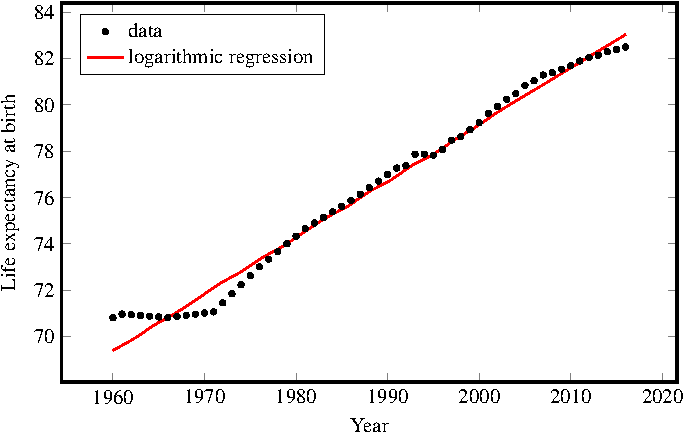
\includegraphics[scale=1.1]{image/12/Australia-life-expectancy.pdf}
\caption{%%
  The life expectancy at birth of Australia between the years $1960$
  and $2016$, inclusive.  The black dots show data provided by the
  World Bank.  The red curve is a graph of
  \Equation{eqn:logarithm:Australia_life_expectancy_formula}.
}
\label{fig:logarithm:Australia_life_expectancy}
\end{figure}

\begin{figure}[!htbp]
\centering
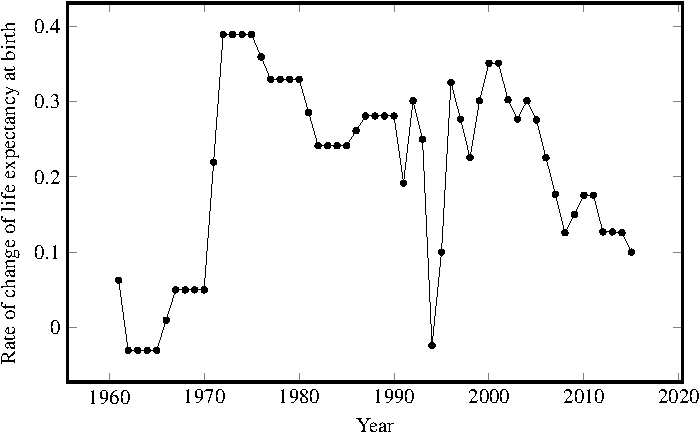
\includegraphics[scale=1.1]{image/12/Australia-life-expectancy-delta.pdf}
\caption{%%
  The rate of change of the life expectancy at birth of Australia
  between the years $1961$ and $2015$, inclusive.  The rates of change
  are based on data provided by the World Bank.
}
\label{fig:logarithm:Australia_rate_of_change_life_expectancy}
\end{figure}

\solutionpart{subprob:logarithm:Australia_life_expectancy_formula}
Let $L(x)$ denote the life expectancy at birth of Australia for the
year $x$.  \Figure{fig:logarithm:Australia_life_expectancy} shows that
$L(x)$ seems to follow a straight line.  This implies that the rates
of change of $L(x)$ are approximately the same.  However,
\Figure{fig:logarithm:Australia_rate_of_change_life_expectancy} shows
that the rates of change of $L(x)$ are not approximately the same.  In
particular, note that from around the year $2000$ onwards the rates of
change are still positive, but they have been decreasing since around
the year $2000$.  In other words, from the year $2000$ onwards $L(x)$
has been increasing at a lower and lower rate each year.  It seems
that $L(x)$ does not approximately follow a straight line, but more
like a logarithmic function.  Logarithmic regression shows that the
life expectancy at birth of Australia from $1960$ up to and including
$2016$ can be modelled as the function
%%
\begin{equation}
\label{eqn:logarithm:Australia_life_expectancy_formula}
L(x)
=
482.3980 \ln x - 3587.4517.
\end{equation}
%%
\Figure{fig:logarithm:Australia_life_expectancy} compares a graph of
\Equation{eqn:logarithm:Australia_life_expectancy_formula} with the
data provided by the World Bank.  The model $L(x)$ has a coefficient
of determination of $R^2 \approx 0.9865$ and a root mean square error
of approximately $0.4662$.

\solutionpart{subprob:logarithm:Australia_GDP_per_capita}
\Figure{fig:logarithm:Australia_GDP_per_capita} shows a
scatter plot of the GDP per capita of Australia between the years
$1960$ and $2016$, inclusive.
\Figure{fig:logarithm:Australia_GDP_per_capita_rate} shows the rate of
change of the GDP per capita.  The horizontal line in the figure
passes through the mean rate of $\mu \approx 650.7070$.

\begin{figure}[!htbp]
\centering
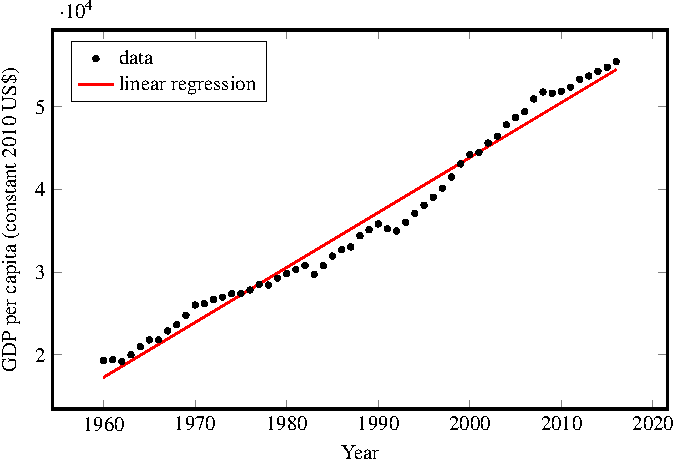
\includegraphics[scale=1.1]{image/12/Australia-gdp-per-capita.pdf}
\caption{%%
  The GDP per capita of Australia from $1960$ to $2016$, inclusive.
  The GDP for each year has been adjusted for inflation with respect
  to the value of the US dollar in the year $2010$.  Note that each
  value on the vertical axis should be multiplied by $10^4$.  The
  black dots show the GDP per capita of Australia as calculated from
  data provided by the World Bank.  The red curve is a graph of
  \Equation{eqn:logarithm:Australia_GPD_per_capita_formula}.
}
\label{fig:logarithm:Australia_GDP_per_capita}
\end{figure}

\begin{figure}[!htbp]
\centering
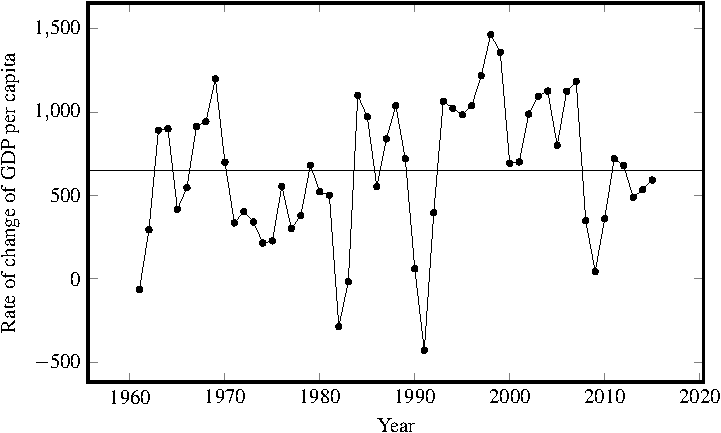
\includegraphics[scale=1.1]{image/12/Australia-gdp-per-capita-delta.pdf}
\caption{%%
  The rate of change of the GDP per capita of Australia between the
  years $1961$ and $2015$, inclusive.  The mean of the rates of change
  is $\mu \approx 650.7070$.  The horizontal line passes through the
  mean on the vertical axis.
}
\label{fig:logarithm:Australia_GDP_per_capita_rate}
\end{figure}

\solutionpart{subprob:logarithm:Australia_GDP_per_capita_formula}
\Figures{fig:logarithm:Australia_GDP_per_capita}{fig:logarithm:Australia_GDP_per_capita_rate}
suggests that the GDP per capita of Australia during the years $1960$
and $2016$, inclusive, can be modelled as a linear function.  As can
be seen in \Figure{fig:logarithm:Australia_GDP_per_capita_rate}, the
rates of change seem to wiggle around the horizontal line through the
mean of $\mu \approx 650.7070$.  Linear regression shows that the GDP
per capita $G(x)$ for the year $x$ can be modelled as
%%
\begin{equation}
\label{eqn:logarithm:Australia_GPD_per_capita_formula}
G(x)
=
665.2450 x - 1286630.9005.
\end{equation}
%%
\Figure{fig:logarithm:Australia_GDP_per_capita} shows a graph of
\Equation{eqn:logarithm:Australia_GPD_per_capita_formula} together
with the actual GDP per capita of Australia.  The function $G(x)$ has
a coefficient of determination of $R^2 \approx 0.9790$ and a root mean
square error of approximately $1601.5557$.

\begin{figure}[!htbp]
\centering
\subfigure[]{
  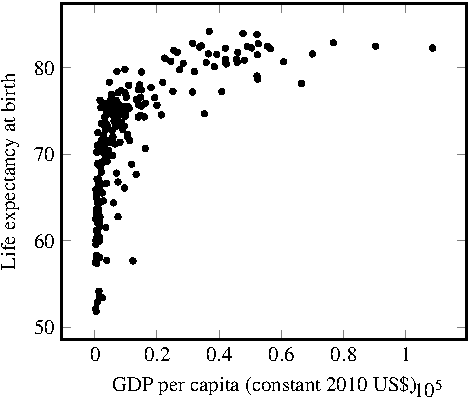
\includegraphics[scale=0.8]{image/12/preston-curve-2016-linear.pdf}
  \label{subfig:logarithm:Preston_curve_2016_linear}
}
%%
%%
\subfigure[]{
  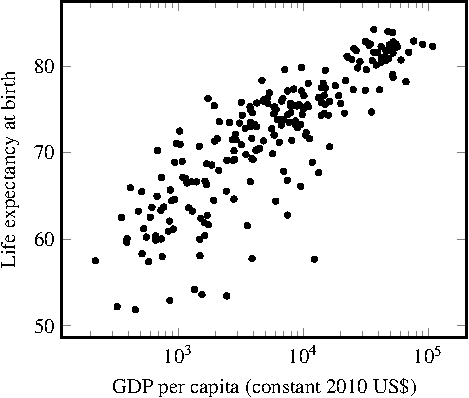
\includegraphics[scale=0.8]{image/12/preston-curve-2016-log.pdf}
  \label{subfig:logarithm:Preston_curve_2016_log}
}
\caption{%%
  The Preston curve for the year $2016$.  Both scatter plots show the
  GDP per capita versus the life expectancy at birth of $224$
  countries.  The GDP per capita has been adjusted to account for
  inflation in terms of the value of the US dollar in the year
  $2010$.  (a)~A scatter plot that uses linear scaling for both of the
  horizontal and vertical axes.  Note that each value on the
  horizontal axis must be multiplied by $10^5$.  (b)~The same scatter
  plot, but using logarithmic and linear scalings for the horizontal
  and vertical axes, respectively.
}
\label{fig:logarithm:Preston_curve_2016}
\end{figure}

\begin{figure}[!htbp]
\centering
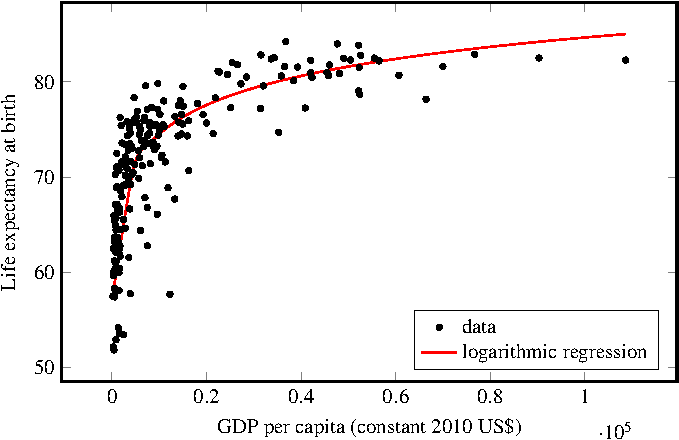
\includegraphics[scale=1.1]{image/12/preston-curve-2016.pdf}
\caption{%%
  The same graph as
  \Figure{subfig:logarithm:Preston_curve_2016_linear}, but the data
  are plotted against the prediction curve.  The black dots show the
  data as provided by the World Bank.  The red curve is a graph of
  \Equation{eqn:logarithm:Preston_curve_2016}.
}
\label{fig:logarithm:Preston_curve_2016_model}
\end{figure}

\solutionpart{subprob:logarithm:Preston_curve_2016_graph_formula}
\Figure{fig:logarithm:Preston_curve_2016} shows two scatter plots of
the GDP per capita versus the life expectancy at birth for the year
$2016$.  \Figure{subfig:logarithm:Preston_curve_2016_log} uses
logarithmic scaling for the horizontal axis and the graph shows that
the data points seem to follow a straight line.  Let $L(x)$ be the
life expectancy at birth for a country that has a GDP per capita of
$x$.  \Figure{subfig:logarithm:Preston_curve_2016_log} suggests that
you can model $L(x)$ as a logarithmic function.  Logarithmic
regression shows that the data points can be modelled as
%%
\begin{equation}
\label{eqn:logarithm:Preston_curve_2016}
L(x)
=
4.4040 \ln x + 33.9595.
\end{equation}
%%
The function $L(x)$ is graphed in
\Figure{fig:logarithm:Preston_curve_2016_model} together with the data
provided by the World Bank.
Equation~\eqref{eqn:logarithm:Preston_curve_2016} has a coefficient of
determination of $R^2 \approx 0.6986$ and a root mean square error of
approximately $4.0940$.

\begin{figure}[!htbp]
\centering
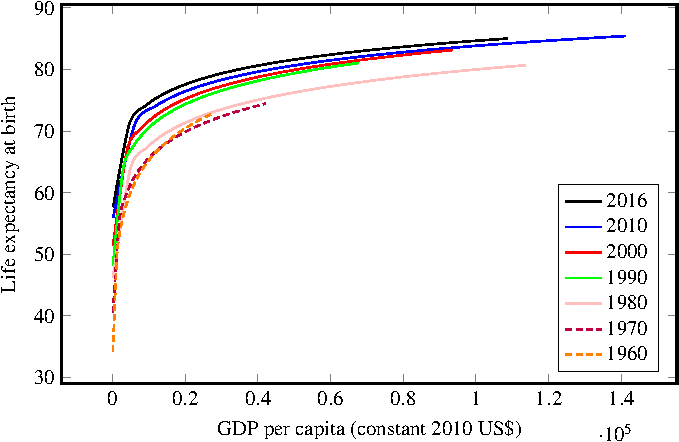
\includegraphics[scale=1.1]{image/12/preston-curve.pdf}
\caption{%%
  The GDP per capita versus the life expectancy of countries around
  the world for each decade since the year $1960$.  The curves are
  graphs of the equations
  in~\eqref{eqn:logarithm:Preston_curve_1960_2016}.  Note that each
  value on the horizontal axis must be multiplied by $10^5$.
}
\label{fig:logarithm:Preston_curve_1960_2016}
\end{figure}

\solutionpart{subprob:logarithm:Preston_curve_1960_2016}
For any year $t$, let $L_t(x)$ be the life expectancy at birth of a
country that has a GDP per capita of $x$.  Using logarithmic
regression on the data sets, you have the following formulae:
%%
\begin{equation}
\label{eqn:logarithm:Preston_curve_1960_2016}
\begin{aligned}
L_{1960}(x)
&=
7.4964 \ln x - 3.8128 \\[4pt]
%%
L_{1970}(x)
&=
6.1543 \ln x + 8.9141 \\[4pt]
%%
L_{1980}(x)
&=
5.3864 \ln x + 17.9890 \\[4pt]
%%
L_{1990}(x)
&=
5.4981 \ln x + 19.8960 \\[4pt]
%%
L_{2000}(x)
&=
5.1534 \ln x + 24.1678 \\[4pt]
%%
L_{2010}(x)
&=
4.5986 \ln x + 30.9028 \\[4pt]
%%
L_{2016}(x)
&=
4.4040 \ln x + 33.9595
\end{aligned}
\end{equation}
%%
The formulae in~\eqref{eqn:logarithm:Preston_curve_1960_2016} are
graphed in \Figure{fig:logarithm:Preston_curve_1960_2016}.

There are a number of points to notice about the graph in
\Figure{fig:logarithm:Preston_curve_1960_2016}.  First, from the year
$1960$ to $2016$ the life expectancy at birth of countries around the
world has increased by approximately ten years.  This is reflected in
the upward shift of the curves in
\Figure{fig:logarithm:Preston_curve_1960_2016}.  Second, for countries
that have a GDP per capita of less than $0.2 \times 10^5 = 20000$, the
figure seems to suggest that a small increase in GDP per capita can
result in a large increase in the life expectancy at birth.  This is
reflected in the steepness of the curves at the left end of the
graph.  However, once a country has reached a certain level of GDP per
capita, say from $0.6 \times 10^5 = 60000$ onwards, any increase in
the GDP per capita would result in a smaller and smaller increase in
the life expectancy at birth.  This is reflected in the right half of
the graph in \Figure{fig:logarithm:Preston_curve_1960_2016}.  Finally,
the greatest increase in life expectancy at birth occurred during the
decade from $1980$ to $1990$.
\end{solution}
}{}

\item\emph{Metasequoia.}
  Dawn redwood, otherwise known as \emph{Metasequoia}, is a type of
  tree that is native to China.  In~2017, a group of researchers
  published their findings on the diameter at breast height~(DBH)
  versus height of $5503$ \emph{Metasequoia} trees found in Hubei,
  China.\footnote{
    The paper is available at
    \url{https://doi.org/10.1371/journal.pone.0182170}.
  }
  The researchers have released a sample of measurements of $500$
  trees; see the data file \code{metasequoia.csv}.
  %%
  \begin{packedenum}
  \item\label{subprob:logistic:metasequoia_height_distribution}
    The heights in the data file \code{metasequoia.csv} range from a
    minimum of $17.35$ metres to a maximum of $45.62$ metres.  To get
    a rough idea of how the heights are spread across the $500$ trees,
    you can place each height measurement in exactly one of several
    classes.  The class $18$ contains all heights $h$ such that
    $17 \leq h < 18$, i.e.~all heights that are at least $17$ metres
    and less than $18$ metres.  The class $19$ contains all heights
    $h$ such that $18 \leq h < 19$.  Similarly, the class $20$
    contains all heights $h$ such that $19 \leq h < 20$.  And so on up
    to and including the class $46$, which contains all heights $h$
    such that $45 \leq h < 46$.  Produce a table that has three
    columns and as many rows as necessary.  Going from left to right,
    the first column should have a heading called ``Class'' and should
    list each of the classes from class $18$ up to and including class
    $46$.  The middle column should have a heading called ``Count''
    and should list for each class the corresponding number of height
    measurements that can be placed in the class.  Finally, the third
    column should have a heading called ``Probability'' and should
    list the corresponding count divided by $500$.  This is the
    observed probability, i.e.~the probability value is derived from
    the data.  For example, the class $18$ should have a count of $2$
    because there are two height measurements that are at least $17$
    metres but less than $18$ metres.  Furthermore, you have a
    probability of $2 / 500 = 0.004$ that a \emph{Metasequoia} tree
    has a height of $h$ metres such that $17 \leq h < 18$.  Remove any
    row that has a count of zero.  Determine the range of tree heights
    that occur the most often in the given sample of $500$ trees.

  \item\label{subprob:logistic:metasequoia_height_mean_stdev}
    Let's calculate some statistics on the heights of the
    \emph{Metasequoia} trees.  First, calculate the mean $\mu$ of the
    $500$ tree heights.  Next, calculate the \emph{standard deviation}
    $\sigma$ of the $500$ tree heights.  Let $h_i$ be the height
    measurement of tree $i$ for $i = \seq{1}{2}{500}$.  The difference
    between the height of tree $i$ and the mean height is $h_i - \mu$.
    Square the difference to get $(h_i - \mu)^2$.  Now add up all the
    squared differences, divide the result by $n - 1$, and take the
    square root to obtain the standard deviation
    \[
    \sigma
    =
    \sqrt{
      \frac{1}{n - 1}
      \sum_{i=1}^n (h_i - \mu)^2
    }
    \]
    where $n = 500$ denotes the number of trees.  Note that the
    standard deviation is similar to the definition of the root mean
    square error.  The main difference is that in the standard
    deviation you divide by $n - 1$, not $n$.  Like the root mean
    square error, the standard deviation gives you an average of how
    much any value~(or tree height) differs from the mean value~(or
    mean tree height).  Determine the mean and standard deviation of
    the $500$ tree heights.  Provide an interpretation of the standard
    deviation of the tree heights.

  \item\label{subprob:logistic:metasequoia_height_normal_plot}
    If you plot the value of the height class versus the corresponding
    observed probability, the points would seem to follow the shape of
    a bell curve.  This bell curve shape is known as the
    \emph{normal distribution} and is also called the
    \emph{Gaussian distribution}.  You can use the following technique
    to fit a normal distribution to your plot.  Let $\mu$ and $\sigma$
    be the mean and standard deviation, respectively, of the tree
    heights.  If the heights of \emph{Metasequoia} trees follow a
    normal distribution, then the probability of observing a
    \emph{Metasequoia} tree of $x$ metres high is
    %%
    \begin{equation}
    \label{eqn:logarithm:metasequoia_normal_distribution}
    P(x)
    =
    \frac{1}{\sigma \sqrt{2 \pi}}
    \exp{
      -
      \frac{
        (x - \mu)^2
      }{
        2 \sigma^2
      }
    }.
    \end{equation}
    %%
    Equation~\eqref{eqn:logarithm:metasequoia_normal_distribution}
    gives you the predicted probability.  The equation can also be
    used to predict the number of \emph{Metasequoia} trees of a
    particular height.  If you have $N$ \emph{Metasequoia} trees,
    \Equation{eqn:logarithm:metasequoia_normal_distribution} predicts
    that you would have $N \cdot P(x)$ trees of height around $x$
    metres.   Letting $x$ be the height class, use
    \Equation{eqn:logarithm:metasequoia_normal_distribution} to fit a
    normal distribution to your plot of height class versus observed
    probability.  In a sample of $500$ \emph{Metasequoia} trees, use
    \Equation{eqn:logarithm:metasequoia_normal_distribution} to
    predict the number of trees that have a height class of $x$
    metres for $x = \seq{18}{19}{46}$.  Calculate the root mean
    square~(RMS) error of the predicted counts.  Provide an
    interpretation of the RMS error.

  \item\label{subprob:logistic:metasequoia_formula}
    Let $H(x)$ be the height~(m) of a \emph{Metasequoia} tree that has
    a DBH of $x$ centimetres.  Use regression to help you derive a
    formula for $H(x)$.  Graph your formula together with a scatter
    plot of the data in the file \code{metasequoia.csv}.  Calculate
    the coefficient of determination and root mean square error of
    your formula.
  \end{packedenum}
\ifbool{showSolution}{
\begin{solution}
\solutionpart{subprob:logistic:metasequoia_height_distribution}
See \Table{tab:logarithm:Metaseqoia}.  The range of tree heights from
at least $24$ metres up to less than $25$ metres occurs the most often
at $56$ trees out of a total of $500$ trees.

\begin{table}[!htbp]
\centering
\begin{tabular}{ccccc} \toprule
Class & Count & Obs. prob. & Pred. prob. & Pred. count \\\midrule
$18$  & $2$   & $0.004$    & $0.013279$  & $6.6394$  \\
$19$  & $5$   & $0.010$    & $0.020096$  & $10.0481$ \\
$20$  & $15$  & $0.030$    & $0.028914$  & $14.4569$ \\
$21$  & $23$  & $0.046$    & $0.039548$  & $19.7739$ \\
$22$  & $31$  & $0.062$    & $0.051425$  & $25.7124$ \\
$23$  & $38$  & $0.076$    & $0.063570$  & $31.7850$ \\
$24$  & $30$  & $0.060$    & $0.074707$  & $37.3537$ \\
$25$  & $56$  & $0.112$    & $0.083465$  & $41.7326$ \\
$26$  & $32$  & $0.064$    & $0.088650$  & $44.3249$ \\
$27$  & $45$  & $0.090$    & $0.089512$  & $44.7559$ \\
$28$  & $42$  & $0.084$    & $0.085924$  & $42.9619$ \\
$29$  & $49$  & $0.098$    & $0.078411$  & $39.2055$ \\
$30$  & $22$  & $0.044$    & $0.068026$  & $34.0128$ \\
$31$  & $25$  & $0.050$    & $0.056104$  & $28.0522$ \\
$32$  & $24$  & $0.048$    & $0.043990$  & $21.9950$ \\
$33$  & $18$  & $0.036$    & $0.032790$  & $16.3949$ \\
$34$  & $14$  & $0.028$    & $0.023236$  & $11.6179$ \\
$35$  & $7$   & $0.014$    & $0.015653$  & $7.8266$  \\
$36$  & $9$   & $0.018$    & $0.010025$  & $5.0125$  \\
$37$  & $5$   & $0.010$    & $0.006104$  & $3.0518$  \\
$38$  & $1$   & $0.002$    & $0.003533$  & $1.7664$  \\
$39$  & $3$   & $0.006$    & $0.001944$  & $0.9720$  \\
$40$  & $1$   & $0.002$    & $0.001017$  & $0.5085$  \\
$41$  & $2$   & $0.004$    & $0.000506$  & $0.2529$  \\
$46$  & $1$   & $0.002$    & $0.000007$  & $0.0036$  \\\bottomrule
\end{tabular}

\caption{%%
  The probability of each height class for $n = 500$
  \emph{Metasequoia} trees.  Given a class $x$, the corresponding
  count $c$ is the number of height measurements $h$ such that
  $x - 1 \leq h < x$.  The observed probability for the class $x$ is
  $c / n$.  The predicted probability is $P(x)$ as defined by the
  normal distribution in
  \Equation{eqn:logarithm:metasequoia_normal_distribution} with a mean
  of $\mu = 26.6913$ and standard deviation $\sigma \approx 4.4461$.
  The predicted count for the class $x$ is $n \cdot P(x)$.
}
\label{tab:logarithm:Metaseqoia}
\end{table}

\solutionpart{subprob:logistic:metasequoia_height_mean_stdev}
The mean and standard deviation of the $500$ tree heights are
$\mu = 26.6913$ and $\sigma \approx 4.4461$, respectively.  The
standard deviation tells you that on average any given tree height is
approximately $4.4461$ metres away from the mean height of $26.6913$
metres.

\begin{figure}[!htbp]
\centering
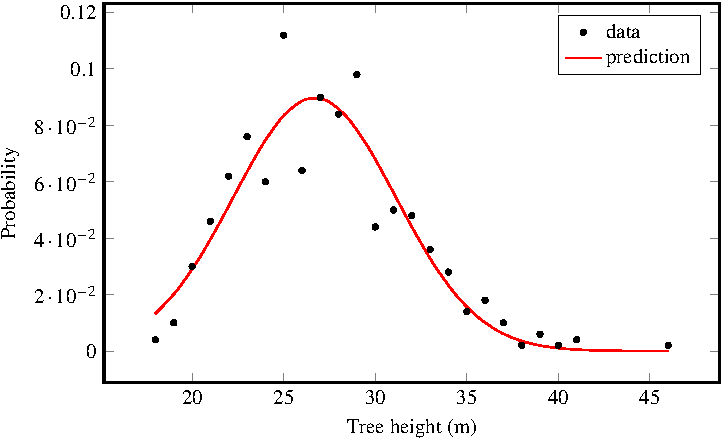
\includegraphics[scale=1.1]{image/12/metasequoia-probability.pdf}
\caption{%%
  The probability of observing a \emph{Metasequoia} tree of a given
  height.  The black dots show the probabilities as calculated using
  the data file \code{metasequoia.csv}.  The red curve is a graph of
  the normal distribution with mean $\mu = 26.6913$ and standard
  deviation $\sigma \approx 4.4461$.
}
\label{fig:logarithm:Metasequoia_normal_distribution}
\end{figure}

\solutionpart{subprob:logistic:metasequoia_height_normal_plot}
\Figure{fig:logarithm:Metasequoia_normal_distribution} shows a fit of
a normal distribution to the empirical probabilities of observing a
\emph{Metasequoia} tree of a given height.  The normal distribution
has a mean of $\mu = 26.6913$ and standard deviation
$\sigma \approx 4.4461$.  The predicted counts are shown in the
right-most column of \Table{tab:logarithm:Metaseqoia}.  The predicted
counts have a root mean square error of approximately $5.7481$.  This
means that, on average, a prediction of the number of
\emph{Metasequoia} trees whose heights belong to a particular class
would differ from the observed number by approximately $5.7481$
trees.

\begin{figure}[!htbp]
\centering
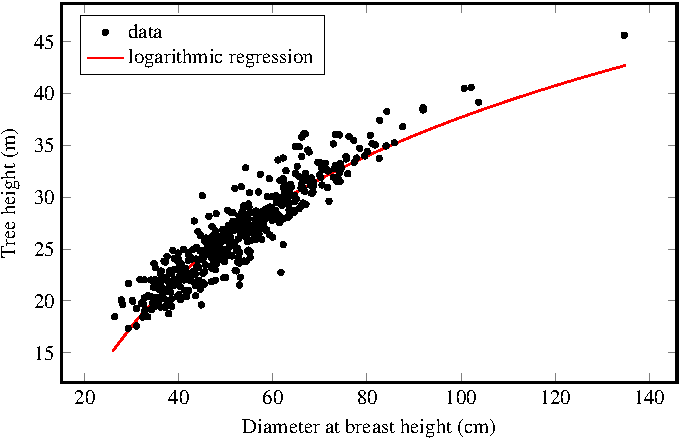
\includegraphics[scale=1.1]{image/12/metasequoia.pdf}
\caption{%%
  The diameter at breast height versus tree height for $500$
  \emph{Metasequoia} trees.  The black dots show a scatter plot of the
  data in the file \code{metasequoia.csv}.  The red curve is a graph
  of \Equation{eqn:logarithm:Metasequoia_log_regression}.
}
\label{fig:logarithm:Metasequoia}
\end{figure}

\solutionpart{subprob:logistic:metasequoia_formula}
Let $H(x)$ be the height in metres of a \emph{Metaseqoia} tree that
has a DBH of $x$ centimetres.  Logarithmic regression on the data in
the file \code{metasequoia.csv} shows that $H(x)$ can be written as
%%
\begin{equation}
\label{eqn:logarithm:Metasequoia_log_regression}
H(x)
=
16.7208 \ln x - 39.3081.
\end{equation}
%%
The function $H(x)$ is graphed in \Figure{fig:logarithm:Metasequoia}
together with a scatter plot of the experimental data for $500$
\emph{Metasequoia} trees.  The
model~\eqref{eqn:logarithm:Metasequoia_log_regression} has a
coefficient of determination of $R^2 \approx 0.8466$ and a root mean
square error of approximately $1.7399$.
\end{solution}
}{}

\begin{table}[!htbp]
\centering
\begin{tabular}{cc} \toprule
Day  & Mean height \\\midrule
$0$  & $10.00$  \\
$7$  & $17.93$  \\
$14$ & $36.36$  \\
$21$ & $67.76$  \\
$28$ & $98.10$  \\
$35$ & $131.00$ \\
$42$ & $169.50$ \\
$49$ & $205.50$ \\
$56$ & $228.30$ \\
$63$ & $247.10$ \\
$70$ & $250.50$ \\
$77$ & $253.80$ \\
$84$ & $254.50$ \\\bottomrule
\end{tabular}

\caption{%%
  The growth of sunflowers, an experiment in~1919 by H.~S.~Reed and
  R.~H.~Holland.  The ``Day'' column lists how many days since the
  start of the experiment.  The ``Mean height'' column lists the
  average height of $58$ sunflowers as measured on the corresponding
  day, where height is measured in centimetres.
}
\label{tab:logarithm:sunflower}
\end{table}

\item\emph{Logistic function.}
  Recall that the logistic function can be written as
  %%
  \begin{equation}
  \label{eqn:logarithm:logistic_function}
  P(t)
  =
  \frac{
    KP_0
  }{
    P_0 + (K - P_0) e^{-rt}
  }.
  \end{equation}
  %%
  The constants $K$, $P_0$, and $r$ are the parameters of the logistic
  function.  Here, $P_0$ denotes the value of the function $P(t)$ at
  time $t = 0$.  If $P(t)$ represents the size of a population at time
  $t$, then $P_0$ is the initial population size.  The maximum value
  of the function $P(t)$ is represented by $K$, i.e.~the population
  size cannot exceed $K$.  Finally, $r$ represents the rate~(as a
  decimal) at which the population size changes.
  %%
  \begin{packedenum}
  \item\label{subprob:logarithm:logistic_equivalent_form}
    Show that \Equation{eqn:logarithm:logistic_function} can also be
    written as
    %%
    \begin{equation}
    \label{eqn:logarithm:logistic_equivalent_form}
    P(t)
    =
    \frac{
      K
    }{
      1 + \parenthesis{\frac{K}{P_0} - 1} e^{-rt}
    }.
    \end{equation}

  \item\label{subprob:logarithm:logistic_Ecoli_example}
    Suppose you initially have $4$ cells of \emph{E.~coli} in a Petri
    dish.  Due to the conditions of the Petri dish, the colony of
    \emph{E.~coli} grows at a rate of $50\%$ per hour, but at any time
    the population size cannot exceed $100$ cells.  If the population
    size of the \emph{E.~coli} colony follows a logistic function, use
    the above information to write a formula for the population size
    at any given time.  Graph your formula for time $t = 0$ up to and
    including $t = 20$.  On the same graph, draw a horizontal line
    through $K = 100$ on the vertical axis.  Explain what you notice
    about the graph.

  \item\label{subprob:logarithm:logistic_sunflower_data}
    In some cases, you are given a data set and must work out whether
    the data can be modelled as a logistic function.  If the data can
    be modelled as a logistic function, you must then use the data to
    estimate the values of the parameters $K$, $P_0$, and $r$.  For
    example, \Table{tab:logarithm:sunflower} shows the mean heights of
    $58$ sunflowers measured at a regular interval of seven
    days.\footnote{
      The data were published in the paper at
      \url{https://doi.org/10.1073/pnas.5.4.135}.
    }
    Produce a scatter plot of the data.  Explain what you notice about
    the trend that the graph shows.

  \item\label{subprob:logarithm:logistic_sunflower_growth_rates}
    As a first step to figuring out whether the data in
    \Table{tab:logarithm:sunflower} can be modelled using a logistic
    function, you must calculate the growth rate for each of the days
    given in the table.  Given a logistic function $P(t)$ of the
    form~\eqref{eqn:logarithm:logistic_function}
    or~\eqref{eqn:logarithm:logistic_equivalent_form}, the rate of
    change per unit time is\footnote{
      Expression~\eqref{eqn:logarithm:logistic_differential_equation}
      is known as the \emph{differential equation} of the logistic
      function.  The solution of the differential equation is the
      logistic function.
    }
    %%
    \begin{equation}
    \label{eqn:logarithm:logistic_differential_equation}
    R
    =
    r P
    \parenthesis*{
      1 - \frac{P}{K}
    }.
    \end{equation}
    %%
    In the case of the sunflower example, you do not know an exact
    expression for the rate of change in the mean height per unit time
    so you must use the given data set to estimate the rate of change
    for each of the listed days.  Similar to
    \Equations{eqn:logarithm:Australia_rate_of_change_life_expectancy}{eqn:logarithm:Australia_GDP_per_capita_rates},
    you let $H(x)$ be the mean height~(cm) of a sunflower on day
    $x \geq 0$ and consider the mean height from the previous
    measurement and the mean height from the measurement following day
    $x$.  Let $u$ and $v$ be the days before and after, respectively,
    day $x$ at which the mean heights are known.  The rate of change
    in $H(x)$ is defined as
    %%
    \begin{equation}
    \label{eqn:logarithm:logistic_sunflower_growth_rate}
    \Delta H(x)
    =
    \frac{
      H(v) - H(u)
    }{
      v - u
    }
    \end{equation}
    %%
    which provides an estimate of how much the mean height has changed
    since the previous measurement.  Note that
    \Equation{eqn:logarithm:logistic_sunflower_growth_rate} cannot be
    used to estimate $\Delta H(0)$ and $\Delta H(84)$ because you
    neither have data for the day before day $x = 0$ nor data for the
    day after day $x = 84$.  Use
    \Equation{eqn:logarithm:logistic_sunflower_growth_rate} to
    estimate the rate of change in the mean heights for all days,
    except for days $x = 0$ and $x = 84$.  Produce a scatter plot of
    the day $x$ versus the rate of change $\Delta H(x)$.  Explain what
    you notice about the graph.

  \item\label{subprob:logarithm:logistic_sunflower_rate_over_function_value}
    In \Equation{eqn:logarithm:logistic_differential_equation}, divide
    both sides by $P$ to get
    %%
    \begin{equation}
    \label{eqn:logarithm:logistic_differential_equation_linear_in_P}
    \begin{aligned}
    \frac{R}{P}
    &=
    r \parenthesis*{1 - \frac{P}{K}} \\[4pt]
    &=
    r - \frac{r}{K} P.
    \end{aligned}
    \end{equation}
    %%
    Suppose that you know the values of the parameters $r$ and $K$.
    Then
    \Equation{eqn:logarithm:logistic_differential_equation_linear_in_P}
    tells you that the ratio $R / P$ is a linear function of $P$.  Not
    only that, but
    \Equation{eqn:logarithm:logistic_differential_equation_linear_in_P}
    tells you two other things in terms of the sunflower example.
    First, for any day $x$ you divide the rate of change $\Delta H(x)$
    in the mean height of a sunflower by the actual mean height
    $H(x)$.  Then you produce a scatter plot of the mean height $H(x)$
    versus the rate of change $\Delta H(x)$ in the mean height.  If
    the plot shows that the dots follow a straight line, then you know
    that the data set can be modelled as a logistic function.  Second,
    if the dots follow a straight line, then use linear regression to
    calculate the values of the vertical intercept $r$ and the
    gradient $m = -r / K$.  Thus the value of $K$ is given by
    $K = -r / m$.  In terms of
    \Equations{eqn:logarithm:logistic_function}{eqn:logarithm:logistic_equivalent_form},
    you have calculated the values of $r$ and $K$ and the initial
    value $P_0$~(or $H_0$ in the sunflower example) can be read off
    from the table of values.  Use the rates of change
    from \Part{subprob:logarithm:logistic_sunflower_growth_rates} to
    calculate the ratios $\frac{\Delta H(x)}{H(x)}$ and produce a
    scatter plot of $H(x)$ versus $\frac{\Delta H(x)}{H(x)}$.  If the
    mean height of a sunflower follows the logistic function
    %%
    \begin{equation}
    \label{eqn:logarithm:logistic_sunflower_formula}
    H(x)
    =
    \frac{
      K
    }{
      1 + \parenthesis*{\frac{K}{H_0} - 1} e^{-rx}
    }
    \end{equation}
    %%
    use linear regression on the known values of $H(x)$ and
    $\frac{\Delta H(x)}{H(x)}$ to estimate the parameters $K$ and
    $r$.  Use the known values of $H_0$, $K$, and $r$ to write a
    formula for the mean height $H(x)$ of a sunflower on day $x$.
    Graph your formula together with the scatter plot
    from \Part{subprob:logarithm:logistic_sunflower_data}.  Calculate
    the coefficient of determination and the root mean square error of
    your formula.
  \end{packedenum}
\ifbool{showSolution}{
\begin{solution}
\solutionpart{subprob:logarithm:logistic_equivalent_form}
In \Equation{eqn:logarithm:logistic_function}, the expression
$(K - P_0)$ can be factorised as
$P_0 \cdot \parenthesis*{\frac{K}{P_0} - 1}$.  Use the latter
expression to write \Equation{eqn:logarithm:logistic_function} as
%%
\begin{align*}
P(t)
&=
\frac{
  KP_0
}{
  P_0 + P_0 \cdot \parenthesis*{\frac{K}{P_0} - 1} e^{-rt}
} \\[4pt]
&=
\frac{P_0}{P_0}
\times
\frac{
  K
}{
  1 + \parenthesis*{\frac{K}{P_0} - 1} e^{-rt}
}
\end{align*}
%%
which simplifies to
\Equation{eqn:logarithm:logistic_equivalent_form}.

\begin{figure}[!htbp]
\centering
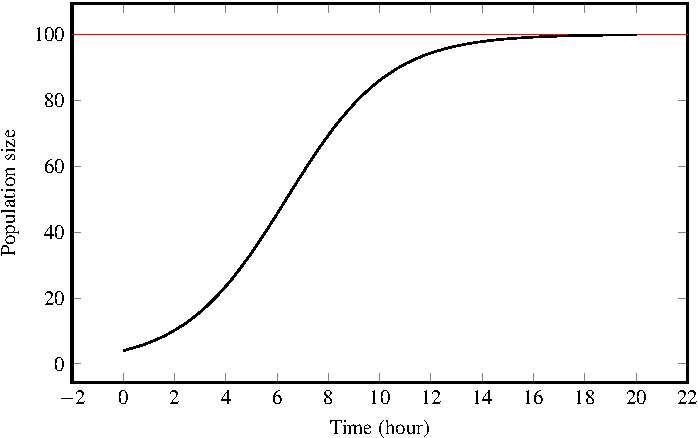
\includegraphics[scale=1.1]{image/12/ecoli.pdf}
\caption{%%
  The time in hours versus the number of cells in a colony of
  \emph{E.~coli}.  The red horizontal line passes through the value of
  $K = 100$ on the vertical axis.
}
\label{fig:logarithm:logistic_Ecoli_population}
\end{figure}

\solutionpart{subprob:logarithm:logistic_Ecoli_example}
Let $P(t)$ be the population size of the \emph{E.~coli} colony at time
$t$ hours, where $t \geq 0$.  You have an initial population size of
$P_0 = 4$.  The growth rate is $50\%$ per hour, which can be written
in decimal form as $r = 50 / 100 = 1 / 2$.  The upper limit on the
population size is $K = 100$.  Substitute the above values into
\Equation{eqn:logarithm:logistic_equivalent_form} and simplify to get
%%
\begin{align*}
P(t)
&=
\frac{
  100
}{
  1 + \parenthesis*{\frac{100}{4} - 1} e^{-\frac{1}{2}t}
} \\[4pt]
&=
\frac{
  100
}{
  1 + 24 e^{-t/2}
}.
\end{align*}
%%
\Figure{fig:logarithm:logistic_Ecoli_population} shows a graph of the
function $P(t)$ for time from $t = 0$ up to and including $t = 20$
hours.  The figure shows that from $t = 0$ up to $t = 100/2 = 50$, the
\emph{E.~coli} population increases according to an exponential
function.  From $t = 50$ onwards, the population levels off like a
logarithmic function.  No matter how much time has passed, the
population size is bounded above by $K = 100$.

\begin{figure}[!htbp]
\centering
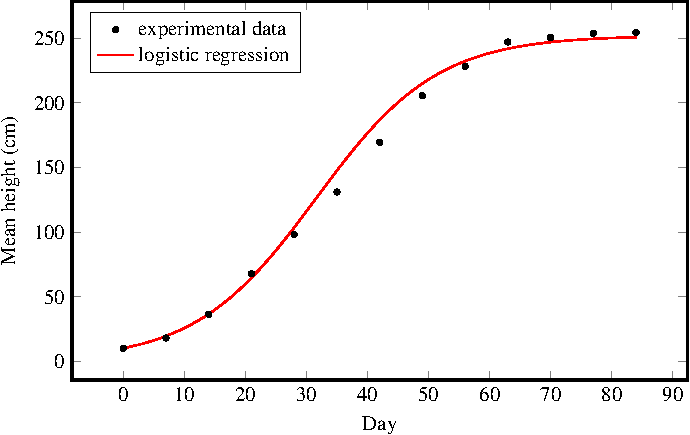
\includegraphics[scale=1.1]{image/12/sunflower.pdf}
\caption{%%
  The growth of $58$ sunflowers.  The black dots show the experimental
  data in \Table{tab:logarithm:sunflower}.  The red curve is a graph
  of
  \Equation{eqn:logarithm:logistic_sunflower_formula_by_regression}.
}
\label{fig:logarithm:sunflower}
\end{figure}

\solutionpart{subprob:logarithm:logistic_sunflower_data}
\Figure{fig:logarithm:sunflower} shows a scatter plot of the data in
\Table{tab:logarithm:sunflower}.  The dots seem to follow an S-shaped
curve that is characteristic of the logistic function.

\begin{figure}[!htbp]
\centering
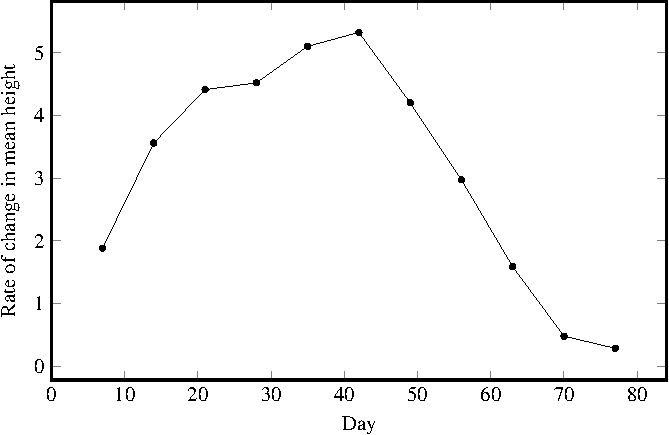
\includegraphics[scale=1.1]{image/12/sunflower-delta.pdf}
\caption{%%
  The rate of change in the mean height of a sunflower.  The rates are
  calculated based on the data in \Table{tab:logarithm:sunflower}.
}
\label{fig:logarithm:logistic_sunflower_delta}
\end{figure}

\solutionpart{subprob:logarithm:logistic_sunflower_growth_rates}
\Figure{fig:logarithm:logistic_sunflower_delta} shows a scatter plot
of the rate of change in the mean height of a sunflower.  The rate of
change increases from day $x = 7$ up to day $x = 42$.  After day
$x = 42$, the rate of change decreases.  The figure suggests that in
the early stages of the growth of a sunflower, the sunflower grows at
a higher and higher rate each day.  After a certain amount of time,
the growth rate of the sunflower reaches a peak and from that time
onwards the growth rate decreases.  That is, after a certain amount of
time the sunflower still increases in height, but by a smaller and
smaller amount each day.

\begin{figure}[!htbp]
\centering
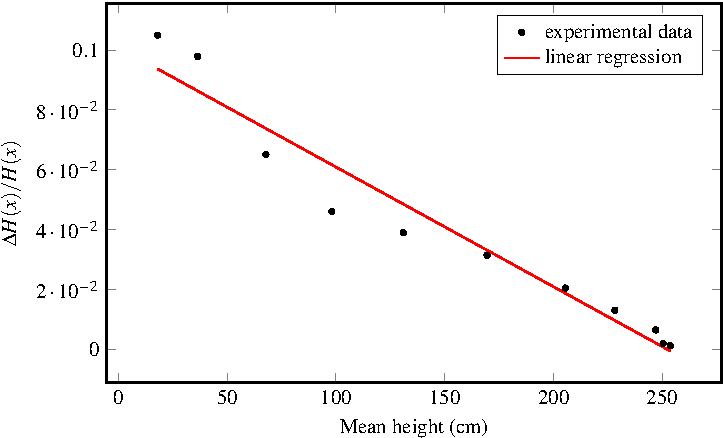
\includegraphics[scale=1.1]{image/12/sunflower-regression.pdf}
\caption{%%
  Linear regression of the mean height $H(x)$ of a sunflower versus
  the ratio $\frac{\Delta H(x)}{H(x)}$.  The black dots represent
  calculations based on the data in \Table{tab:logarithm:sunflower}.
  The red line shows a graph of
  \Equation{eqn:logarithm:logistic_sunflower_regression}.
}
\label{fig:logarithm:logistic_sunflower_regression}
\end{figure}

\solutionpart{subprob:logarithm:logistic_sunflower_rate_over_function_value}
\Figure{fig:logarithm:logistic_sunflower_regression} shows a scatter
plot of the mean height $H(x)$ versus the ratio
$\frac{\Delta H(x)}{H(x)}$.  The black dots in the figure seem to
follow a straight line and linear regression results in the function
%%
\begin{equation}
\label{eqn:logarithm:logistic_sunflower_regression}
\frac{\Delta H(x)}{H(x)}
=
-0.0004 h + 0.1009
\end{equation}
%%
where the variable $h$ denotes the mean height in centimetres.  The
linear function is graphed in
\Figure{fig:logarithm:logistic_sunflower_regression}.  If the
sunflower data set follows the logistic
\Equation{eqn:logarithm:logistic_sunflower_formula}, the parameters
$r$ and $K$ can be estimated as $r \approx 0.1009$ and
$K \approx 252.0837$ and the initial height is $H_0 = 10$ centimetres.
Then the mean height $H(x)$ of a sunflower on day $x$ can be written
as
%%
\begin{equation}
\label{eqn:logarithm:logistic_sunflower_formula_by_regression}
H(x)
=
\frac{
  252.0837
}{
  1 + 24.2083 e^{-0.1009 x}
}.
\end{equation}
%%
The function is graphed in \Figure{fig:logarithm:sunflower} together
with the experimental data from \Table{tab:logarithm:sunflower}.  The
model~\eqref{eqn:logarithm:logistic_sunflower_formula_by_regression}
has a coefficient of determination of $R^2 \approx 0.9472$ and a root
mean square error of approximately $7.8097$.
\end{solution}
}{}
\end{problem}

\end{document}
